\documentclass[twoside]{book}

% Packages required by doxygen
\usepackage{fixltx2e}
\usepackage{calc}
\usepackage{doxygen}
\usepackage[export]{adjustbox} % also loads graphicx
\usepackage{graphicx}
\usepackage[utf8]{inputenc}
\usepackage{makeidx}
\usepackage{multicol}
\usepackage{multirow}
\PassOptionsToPackage{warn}{textcomp}
\usepackage{textcomp}
\usepackage[nointegrals]{wasysym}
\usepackage[table]{xcolor}

% Font selection
\usepackage[T1]{fontenc}
\usepackage[scaled=.90]{helvet}
\usepackage{courier}
\usepackage{amssymb}
\usepackage{sectsty}
\renewcommand{\familydefault}{\sfdefault}
\allsectionsfont{%
  \fontseries{bc}\selectfont%
  \color{darkgray}%
}
\renewcommand{\DoxyLabelFont}{%
  \fontseries{bc}\selectfont%
  \color{darkgray}%
}
\newcommand{\+}{\discretionary{\mbox{\scriptsize$\hookleftarrow$}}{}{}}

% Page & text layout
\usepackage{geometry}
\geometry{%
  a4paper,%
  top=2.5cm,%
  bottom=2.5cm,%
  left=2.5cm,%
  right=2.5cm%
}
\tolerance=750
\hfuzz=15pt
\hbadness=750
\setlength{\emergencystretch}{15pt}
\setlength{\parindent}{0cm}
\setlength{\parskip}{3ex plus 2ex minus 2ex}
\makeatletter
\renewcommand{\paragraph}{%
  \@startsection{paragraph}{4}{0ex}{-1.0ex}{1.0ex}{%
    \normalfont\normalsize\bfseries\SS@parafont%
  }%
}
\renewcommand{\subparagraph}{%
  \@startsection{subparagraph}{5}{0ex}{-1.0ex}{1.0ex}{%
    \normalfont\normalsize\bfseries\SS@subparafont%
  }%
}
\makeatother

% Headers & footers
\usepackage{fancyhdr}
\pagestyle{fancyplain}
\fancyhead[LE]{\fancyplain{}{\bfseries\thepage}}
\fancyhead[CE]{\fancyplain{}{}}
\fancyhead[RE]{\fancyplain{}{\bfseries\leftmark}}
\fancyhead[LO]{\fancyplain{}{\bfseries\rightmark}}
\fancyhead[CO]{\fancyplain{}{}}
\fancyhead[RO]{\fancyplain{}{\bfseries\thepage}}
\fancyfoot[LE]{\fancyplain{}{}}
\fancyfoot[CE]{\fancyplain{}{}}
\fancyfoot[RE]{\fancyplain{}{\bfseries\scriptsize Generated by Doxygen }}
\fancyfoot[LO]{\fancyplain{}{\bfseries\scriptsize Generated by Doxygen }}
\fancyfoot[CO]{\fancyplain{}{}}
\fancyfoot[RO]{\fancyplain{}{}}
\renewcommand{\footrulewidth}{0.4pt}
\renewcommand{\chaptermark}[1]{%
  \markboth{#1}{}%
}
\renewcommand{\sectionmark}[1]{%
  \markright{\thesection\ #1}%
}

% Indices & bibliography
\usepackage{natbib}
\usepackage[titles]{tocloft}
\setcounter{tocdepth}{3}
\setcounter{secnumdepth}{5}
\makeindex

% Hyperlinks (required, but should be loaded last)
\usepackage{ifpdf}
\ifpdf
  \usepackage[pdftex,pagebackref=true]{hyperref}
\else
  \usepackage[ps2pdf,pagebackref=true]{hyperref}
\fi
\hypersetup{%
  colorlinks=true,%
  linkcolor=blue,%
  citecolor=blue,%
  unicode%
}

% Custom commands
\newcommand{\clearemptydoublepage}{%
  \newpage{\pagestyle{empty}\cleardoublepage}%
}

\usepackage{caption}
\captionsetup{labelsep=space,justification=centering,font={bf},singlelinecheck=off,skip=4pt,position=top}

%===== C O N T E N T S =====

\begin{document}

% Titlepage & ToC
\hypersetup{pageanchor=false,
             bookmarksnumbered=true,
             pdfencoding=unicode
            }
\pagenumbering{roman}
\begin{titlepage}
\vspace*{7cm}
\begin{center}%
{\Large Dauntless Concepts Underwater L\+ED Project \\[1ex]\large 1.\+0 }\\
\vspace*{1cm}
{\large Generated by Doxygen 1.8.11}\\
\end{center}
\end{titlepage}
\clearemptydoublepage
\tableofcontents
\clearemptydoublepage
\pagenumbering{arabic}
\hypersetup{pageanchor=true}

%--- Begin generated contents ---
\chapter{Class Index}
\section{Class List}
Here are the classes, structs, unions and interfaces with brief descriptions\+:\begin{DoxyCompactList}
\item\contentsline{section}{\hyperlink{structFlashMemoryData}{Flash\+Memory\+Data} }{\pageref{structFlashMemoryData}}{}
\item\contentsline{section}{\hyperlink{structSCStatus}{S\+C\+Status} }{\pageref{structSCStatus}}{}
\item\contentsline{section}{\hyperlink{structsensorFeedback}{sensor\+Feedback} \\*Sensor\+Feedback struct Description }{\pageref{structsensorFeedback}}{}
\item\contentsline{section}{\hyperlink{classTimerClass}{Timer\+Class} }{\pageref{classTimerClass}}{}
\end{DoxyCompactList}

\chapter{File Index}
\section{File List}
Here is a list of all files with brief descriptions\+:\begin{DoxyCompactList}
\item\contentsline{section}{\hyperlink{FaultHandler_8cpp}{Fault\+Handler.\+cpp} }{\pageref{FaultHandler_8cpp}}{}
\item\contentsline{section}{\hyperlink{FaultHandler_8h}{Fault\+Handler.\+h} }{\pageref{FaultHandler_8h}}{}
\item\contentsline{section}{\hyperlink{Globals_8cpp}{Globals.\+cpp} }{\pageref{Globals_8cpp}}{}
\item\contentsline{section}{\hyperlink{Globals_8h}{Globals.\+h} }{\pageref{Globals_8h}}{}
\item\contentsline{section}{\hyperlink{HardwareConfiguration_8h}{Hardware\+Configuration.\+h} }{\pageref{HardwareConfiguration_8h}}{}
\item\contentsline{section}{\hyperlink{LEDControlManager_8cpp}{L\+E\+D\+Control\+Manager.\+cpp} }{\pageref{LEDControlManager_8cpp}}{}
\item\contentsline{section}{\hyperlink{LEDControlManager_8h}{L\+E\+D\+Control\+Manager.\+h} }{\pageref{LEDControlManager_8h}}{}
\item\contentsline{section}{\hyperlink{Memory_8c}{Memory.\+c} }{\pageref{Memory_8c}}{}
\item\contentsline{section}{\hyperlink{Memory_8h}{Memory.\+h} }{\pageref{Memory_8h}}{}
\item\contentsline{section}{\hyperlink{PinDefinitions_8h}{Pin\+Definitions.\+h} }{\pageref{PinDefinitions_8h}}{}
\item\contentsline{section}{\hyperlink{SensorManager_8cpp}{Sensor\+Manager.\+cpp} }{\pageref{SensorManager_8cpp}}{}
\item\contentsline{section}{\hyperlink{SensorManager_8h}{Sensor\+Manager.\+h} }{\pageref{SensorManager_8h}}{}
\item\contentsline{section}{\hyperlink{SerialDebug_8cpp}{Serial\+Debug.\+cpp} }{\pageref{SerialDebug_8cpp}}{}
\item\contentsline{section}{\hyperlink{SerialDebug_8h}{Serial\+Debug.\+h} }{\pageref{SerialDebug_8h}}{}
\item\contentsline{section}{\hyperlink{States_8cpp}{States.\+cpp} }{\pageref{States_8cpp}}{}
\item\contentsline{section}{\hyperlink{States_8h}{States.\+h} }{\pageref{States_8h}}{}
\end{DoxyCompactList}

\chapter{Class Documentation}
\hypertarget{structFlashMemoryData}{}\section{Flash\+Memory\+Data Struct Reference}
\label{structFlashMemoryData}\index{Flash\+Memory\+Data@{Flash\+Memory\+Data}}


{\ttfamily \#include $<$Globals.\+h$>$}

\subsection*{Public Attributes}
\begin{DoxyCompactItemize}
\item 
char \hyperlink{structFlashMemoryData_a705e1d416a34d2ccc01ceefb29a87107}{part\+Number} \mbox{[}10\mbox{]}
\item 
char \hyperlink{structFlashMemoryData_aa1979cdc22a417ffc32a019be7b471b8}{driver\+Serial\+Number} \mbox{[}8\mbox{]}
\item 
char \hyperlink{structFlashMemoryData_acc795cc627dad7b6e2e0eeb0c7adf9f7}{driver\+Name} \mbox{[}11\mbox{]}
\item 
char \hyperlink{structFlashMemoryData_aa29665746360a0d2a805debad70bd35a}{red\+L\+E\+D\+Value}
\item 
char \hyperlink{structFlashMemoryData_ace37d1ae35660e2af893530d50b24c48}{green\+L\+E\+D\+Value}
\item 
char \hyperlink{structFlashMemoryData_a740528a2ae1beb940f4f3286c4a31438}{blue\+L\+E\+D\+Value}
\item 
unsigned char \hyperlink{structFlashMemoryData_aa0c7f427a26e432cccf13da23fd5d447}{mode}
\item 
unsigned int \hyperlink{structFlashMemoryData_a4fb83987f5c20eb21e133bb968817421}{mode\+Timing1}
\item 
unsigned int \hyperlink{structFlashMemoryData_adb10643e88fbd03db295b843c913883e}{mode\+Timing2}
\item 
unsigned int \hyperlink{structFlashMemoryData_abf400b8235e203ec4ccfdfa5aedcdcec}{mode\+Timing3}
\item 
unsigned long int \hyperlink{structFlashMemoryData_a4bec4294af40d5b6ff0949a7c0af9620}{time\+Of\+Use\+Min}
\item 
bool \hyperlink{structFlashMemoryData_a3b88de12ed87ebc9b4e5ee272dc4389f}{rf\+Telemetry\+Enabled}
\item 
bool \hyperlink{structFlashMemoryData_a4bb2dc9e647ff6663d74cf6c2294f3ab}{serial\+Telemetry\+Enabled}
\item 
bool \hyperlink{structFlashMemoryData_a59ac51257a62821b13f8df0d21b86135}{serial\+Debugging\+Level}
\item 
bool \hyperlink{structFlashMemoryData_adcf63c0ba25e843a3e2e0e0f1bcad4e8}{test\+Data\+Output\+Enabled}
\item 
bool \hyperlink{structFlashMemoryData_a3b5553fc5eb53805c6f10a7c1a80dd83}{voltage\+Protection\+Enabled}
\item 
bool \hyperlink{structFlashMemoryData_aede7cdfaeb691f39ff50b350d1e0b3b9}{temperature\+Protection\+Enabled}
\item 
bool \hyperlink{structFlashMemoryData_aa5ccce295f4c2cf838962fbfca9ee9a9}{data\+Refresh\+Time\+Met}
\item 
unsigned int \hyperlink{structFlashMemoryData_a25f722ef2d2742bc8881ae5164af3c04}{debug\+Data\+Refresh\+Rate\+Ms}
\end{DoxyCompactItemize}


\subsection{Member Data Documentation}
\index{Flash\+Memory\+Data@{Flash\+Memory\+Data}!blue\+L\+E\+D\+Value@{blue\+L\+E\+D\+Value}}
\index{blue\+L\+E\+D\+Value@{blue\+L\+E\+D\+Value}!Flash\+Memory\+Data@{Flash\+Memory\+Data}}
\subsubsection[{\texorpdfstring{blue\+L\+E\+D\+Value}{blueLEDValue}}]{\setlength{\rightskip}{0pt plus 5cm}char Flash\+Memory\+Data\+::blue\+L\+E\+D\+Value}\hypertarget{structFlashMemoryData_a740528a2ae1beb940f4f3286c4a31438}{}\label{structFlashMemoryData_a740528a2ae1beb940f4f3286c4a31438}
\index{Flash\+Memory\+Data@{Flash\+Memory\+Data}!data\+Refresh\+Time\+Met@{data\+Refresh\+Time\+Met}}
\index{data\+Refresh\+Time\+Met@{data\+Refresh\+Time\+Met}!Flash\+Memory\+Data@{Flash\+Memory\+Data}}
\subsubsection[{\texorpdfstring{data\+Refresh\+Time\+Met}{dataRefreshTimeMet}}]{\setlength{\rightskip}{0pt plus 5cm}bool Flash\+Memory\+Data\+::data\+Refresh\+Time\+Met}\hypertarget{structFlashMemoryData_aa5ccce295f4c2cf838962fbfca9ee9a9}{}\label{structFlashMemoryData_aa5ccce295f4c2cf838962fbfca9ee9a9}
\index{Flash\+Memory\+Data@{Flash\+Memory\+Data}!debug\+Data\+Refresh\+Rate\+Ms@{debug\+Data\+Refresh\+Rate\+Ms}}
\index{debug\+Data\+Refresh\+Rate\+Ms@{debug\+Data\+Refresh\+Rate\+Ms}!Flash\+Memory\+Data@{Flash\+Memory\+Data}}
\subsubsection[{\texorpdfstring{debug\+Data\+Refresh\+Rate\+Ms}{debugDataRefreshRateMs}}]{\setlength{\rightskip}{0pt plus 5cm}unsigned int Flash\+Memory\+Data\+::debug\+Data\+Refresh\+Rate\+Ms}\hypertarget{structFlashMemoryData_a25f722ef2d2742bc8881ae5164af3c04}{}\label{structFlashMemoryData_a25f722ef2d2742bc8881ae5164af3c04}
\index{Flash\+Memory\+Data@{Flash\+Memory\+Data}!driver\+Name@{driver\+Name}}
\index{driver\+Name@{driver\+Name}!Flash\+Memory\+Data@{Flash\+Memory\+Data}}
\subsubsection[{\texorpdfstring{driver\+Name}{driverName}}]{\setlength{\rightskip}{0pt plus 5cm}char Flash\+Memory\+Data\+::driver\+Name\mbox{[}11\mbox{]}}\hypertarget{structFlashMemoryData_acc795cc627dad7b6e2e0eeb0c7adf9f7}{}\label{structFlashMemoryData_acc795cc627dad7b6e2e0eeb0c7adf9f7}
\index{Flash\+Memory\+Data@{Flash\+Memory\+Data}!driver\+Serial\+Number@{driver\+Serial\+Number}}
\index{driver\+Serial\+Number@{driver\+Serial\+Number}!Flash\+Memory\+Data@{Flash\+Memory\+Data}}
\subsubsection[{\texorpdfstring{driver\+Serial\+Number}{driverSerialNumber}}]{\setlength{\rightskip}{0pt plus 5cm}char Flash\+Memory\+Data\+::driver\+Serial\+Number\mbox{[}8\mbox{]}}\hypertarget{structFlashMemoryData_aa1979cdc22a417ffc32a019be7b471b8}{}\label{structFlashMemoryData_aa1979cdc22a417ffc32a019be7b471b8}
\index{Flash\+Memory\+Data@{Flash\+Memory\+Data}!green\+L\+E\+D\+Value@{green\+L\+E\+D\+Value}}
\index{green\+L\+E\+D\+Value@{green\+L\+E\+D\+Value}!Flash\+Memory\+Data@{Flash\+Memory\+Data}}
\subsubsection[{\texorpdfstring{green\+L\+E\+D\+Value}{greenLEDValue}}]{\setlength{\rightskip}{0pt plus 5cm}char Flash\+Memory\+Data\+::green\+L\+E\+D\+Value}\hypertarget{structFlashMemoryData_ace37d1ae35660e2af893530d50b24c48}{}\label{structFlashMemoryData_ace37d1ae35660e2af893530d50b24c48}
\index{Flash\+Memory\+Data@{Flash\+Memory\+Data}!mode@{mode}}
\index{mode@{mode}!Flash\+Memory\+Data@{Flash\+Memory\+Data}}
\subsubsection[{\texorpdfstring{mode}{mode}}]{\setlength{\rightskip}{0pt plus 5cm}unsigned char Flash\+Memory\+Data\+::mode}\hypertarget{structFlashMemoryData_aa0c7f427a26e432cccf13da23fd5d447}{}\label{structFlashMemoryData_aa0c7f427a26e432cccf13da23fd5d447}
\index{Flash\+Memory\+Data@{Flash\+Memory\+Data}!mode\+Timing1@{mode\+Timing1}}
\index{mode\+Timing1@{mode\+Timing1}!Flash\+Memory\+Data@{Flash\+Memory\+Data}}
\subsubsection[{\texorpdfstring{mode\+Timing1}{modeTiming1}}]{\setlength{\rightskip}{0pt plus 5cm}unsigned int Flash\+Memory\+Data\+::mode\+Timing1}\hypertarget{structFlashMemoryData_a4fb83987f5c20eb21e133bb968817421}{}\label{structFlashMemoryData_a4fb83987f5c20eb21e133bb968817421}
\index{Flash\+Memory\+Data@{Flash\+Memory\+Data}!mode\+Timing2@{mode\+Timing2}}
\index{mode\+Timing2@{mode\+Timing2}!Flash\+Memory\+Data@{Flash\+Memory\+Data}}
\subsubsection[{\texorpdfstring{mode\+Timing2}{modeTiming2}}]{\setlength{\rightskip}{0pt plus 5cm}unsigned int Flash\+Memory\+Data\+::mode\+Timing2}\hypertarget{structFlashMemoryData_adb10643e88fbd03db295b843c913883e}{}\label{structFlashMemoryData_adb10643e88fbd03db295b843c913883e}
\index{Flash\+Memory\+Data@{Flash\+Memory\+Data}!mode\+Timing3@{mode\+Timing3}}
\index{mode\+Timing3@{mode\+Timing3}!Flash\+Memory\+Data@{Flash\+Memory\+Data}}
\subsubsection[{\texorpdfstring{mode\+Timing3}{modeTiming3}}]{\setlength{\rightskip}{0pt plus 5cm}unsigned int Flash\+Memory\+Data\+::mode\+Timing3}\hypertarget{structFlashMemoryData_abf400b8235e203ec4ccfdfa5aedcdcec}{}\label{structFlashMemoryData_abf400b8235e203ec4ccfdfa5aedcdcec}
\index{Flash\+Memory\+Data@{Flash\+Memory\+Data}!part\+Number@{part\+Number}}
\index{part\+Number@{part\+Number}!Flash\+Memory\+Data@{Flash\+Memory\+Data}}
\subsubsection[{\texorpdfstring{part\+Number}{partNumber}}]{\setlength{\rightskip}{0pt plus 5cm}char Flash\+Memory\+Data\+::part\+Number\mbox{[}10\mbox{]}}\hypertarget{structFlashMemoryData_a705e1d416a34d2ccc01ceefb29a87107}{}\label{structFlashMemoryData_a705e1d416a34d2ccc01ceefb29a87107}
\index{Flash\+Memory\+Data@{Flash\+Memory\+Data}!red\+L\+E\+D\+Value@{red\+L\+E\+D\+Value}}
\index{red\+L\+E\+D\+Value@{red\+L\+E\+D\+Value}!Flash\+Memory\+Data@{Flash\+Memory\+Data}}
\subsubsection[{\texorpdfstring{red\+L\+E\+D\+Value}{redLEDValue}}]{\setlength{\rightskip}{0pt plus 5cm}char Flash\+Memory\+Data\+::red\+L\+E\+D\+Value}\hypertarget{structFlashMemoryData_aa29665746360a0d2a805debad70bd35a}{}\label{structFlashMemoryData_aa29665746360a0d2a805debad70bd35a}
\index{Flash\+Memory\+Data@{Flash\+Memory\+Data}!rf\+Telemetry\+Enabled@{rf\+Telemetry\+Enabled}}
\index{rf\+Telemetry\+Enabled@{rf\+Telemetry\+Enabled}!Flash\+Memory\+Data@{Flash\+Memory\+Data}}
\subsubsection[{\texorpdfstring{rf\+Telemetry\+Enabled}{rfTelemetryEnabled}}]{\setlength{\rightskip}{0pt plus 5cm}bool Flash\+Memory\+Data\+::rf\+Telemetry\+Enabled}\hypertarget{structFlashMemoryData_a3b88de12ed87ebc9b4e5ee272dc4389f}{}\label{structFlashMemoryData_a3b88de12ed87ebc9b4e5ee272dc4389f}
\index{Flash\+Memory\+Data@{Flash\+Memory\+Data}!serial\+Debugging\+Level@{serial\+Debugging\+Level}}
\index{serial\+Debugging\+Level@{serial\+Debugging\+Level}!Flash\+Memory\+Data@{Flash\+Memory\+Data}}
\subsubsection[{\texorpdfstring{serial\+Debugging\+Level}{serialDebuggingLevel}}]{\setlength{\rightskip}{0pt plus 5cm}bool Flash\+Memory\+Data\+::serial\+Debugging\+Level}\hypertarget{structFlashMemoryData_a59ac51257a62821b13f8df0d21b86135}{}\label{structFlashMemoryData_a59ac51257a62821b13f8df0d21b86135}
\index{Flash\+Memory\+Data@{Flash\+Memory\+Data}!serial\+Telemetry\+Enabled@{serial\+Telemetry\+Enabled}}
\index{serial\+Telemetry\+Enabled@{serial\+Telemetry\+Enabled}!Flash\+Memory\+Data@{Flash\+Memory\+Data}}
\subsubsection[{\texorpdfstring{serial\+Telemetry\+Enabled}{serialTelemetryEnabled}}]{\setlength{\rightskip}{0pt plus 5cm}bool Flash\+Memory\+Data\+::serial\+Telemetry\+Enabled}\hypertarget{structFlashMemoryData_a4bb2dc9e647ff6663d74cf6c2294f3ab}{}\label{structFlashMemoryData_a4bb2dc9e647ff6663d74cf6c2294f3ab}
\index{Flash\+Memory\+Data@{Flash\+Memory\+Data}!temperature\+Protection\+Enabled@{temperature\+Protection\+Enabled}}
\index{temperature\+Protection\+Enabled@{temperature\+Protection\+Enabled}!Flash\+Memory\+Data@{Flash\+Memory\+Data}}
\subsubsection[{\texorpdfstring{temperature\+Protection\+Enabled}{temperatureProtectionEnabled}}]{\setlength{\rightskip}{0pt plus 5cm}bool Flash\+Memory\+Data\+::temperature\+Protection\+Enabled}\hypertarget{structFlashMemoryData_aede7cdfaeb691f39ff50b350d1e0b3b9}{}\label{structFlashMemoryData_aede7cdfaeb691f39ff50b350d1e0b3b9}
\index{Flash\+Memory\+Data@{Flash\+Memory\+Data}!test\+Data\+Output\+Enabled@{test\+Data\+Output\+Enabled}}
\index{test\+Data\+Output\+Enabled@{test\+Data\+Output\+Enabled}!Flash\+Memory\+Data@{Flash\+Memory\+Data}}
\subsubsection[{\texorpdfstring{test\+Data\+Output\+Enabled}{testDataOutputEnabled}}]{\setlength{\rightskip}{0pt plus 5cm}bool Flash\+Memory\+Data\+::test\+Data\+Output\+Enabled}\hypertarget{structFlashMemoryData_adcf63c0ba25e843a3e2e0e0f1bcad4e8}{}\label{structFlashMemoryData_adcf63c0ba25e843a3e2e0e0f1bcad4e8}
\index{Flash\+Memory\+Data@{Flash\+Memory\+Data}!time\+Of\+Use\+Min@{time\+Of\+Use\+Min}}
\index{time\+Of\+Use\+Min@{time\+Of\+Use\+Min}!Flash\+Memory\+Data@{Flash\+Memory\+Data}}
\subsubsection[{\texorpdfstring{time\+Of\+Use\+Min}{timeOfUseMin}}]{\setlength{\rightskip}{0pt plus 5cm}unsigned long int Flash\+Memory\+Data\+::time\+Of\+Use\+Min}\hypertarget{structFlashMemoryData_a4bec4294af40d5b6ff0949a7c0af9620}{}\label{structFlashMemoryData_a4bec4294af40d5b6ff0949a7c0af9620}
\index{Flash\+Memory\+Data@{Flash\+Memory\+Data}!voltage\+Protection\+Enabled@{voltage\+Protection\+Enabled}}
\index{voltage\+Protection\+Enabled@{voltage\+Protection\+Enabled}!Flash\+Memory\+Data@{Flash\+Memory\+Data}}
\subsubsection[{\texorpdfstring{voltage\+Protection\+Enabled}{voltageProtectionEnabled}}]{\setlength{\rightskip}{0pt plus 5cm}bool Flash\+Memory\+Data\+::voltage\+Protection\+Enabled}\hypertarget{structFlashMemoryData_a3b5553fc5eb53805c6f10a7c1a80dd83}{}\label{structFlashMemoryData_a3b5553fc5eb53805c6f10a7c1a80dd83}


The documentation for this struct was generated from the following file\+:\begin{DoxyCompactItemize}
\item 
\hyperlink{Globals_8h}{Globals.\+h}\end{DoxyCompactItemize}

\hypertarget{structSCStatus}{}\section{S\+C\+Status Struct Reference}
\label{structSCStatus}\index{S\+C\+Status@{S\+C\+Status}}


{\ttfamily \#include $<$Globals.\+h$>$}

\subsection*{Public Attributes}
\begin{DoxyCompactItemize}
\item 
char \hyperlink{structSCStatus_abb046ef0909fde514e42f8c2396dd4c6}{L\+E\+D\+Intensity}
\item 
bool \hyperlink{structSCStatus_aa2d12cf60ea52e17e2827246821e3af7}{S\+Cdriver\+Fault\+Flag}
\end{DoxyCompactItemize}


\subsection{Member Data Documentation}
\index{S\+C\+Status@{S\+C\+Status}!L\+E\+D\+Intensity@{L\+E\+D\+Intensity}}
\index{L\+E\+D\+Intensity@{L\+E\+D\+Intensity}!S\+C\+Status@{S\+C\+Status}}
\subsubsection[{\texorpdfstring{L\+E\+D\+Intensity}{LEDIntensity}}]{\setlength{\rightskip}{0pt plus 5cm}char S\+C\+Status\+::\+L\+E\+D\+Intensity}\hypertarget{structSCStatus_abb046ef0909fde514e42f8c2396dd4c6}{}\label{structSCStatus_abb046ef0909fde514e42f8c2396dd4c6}
\index{S\+C\+Status@{S\+C\+Status}!S\+Cdriver\+Fault\+Flag@{S\+Cdriver\+Fault\+Flag}}
\index{S\+Cdriver\+Fault\+Flag@{S\+Cdriver\+Fault\+Flag}!S\+C\+Status@{S\+C\+Status}}
\subsubsection[{\texorpdfstring{S\+Cdriver\+Fault\+Flag}{SCdriverFaultFlag}}]{\setlength{\rightskip}{0pt plus 5cm}bool S\+C\+Status\+::\+S\+Cdriver\+Fault\+Flag}\hypertarget{structSCStatus_aa2d12cf60ea52e17e2827246821e3af7}{}\label{structSCStatus_aa2d12cf60ea52e17e2827246821e3af7}


The documentation for this struct was generated from the following file\+:\begin{DoxyCompactItemize}
\item 
\hyperlink{Globals_8h}{Globals.\+h}\end{DoxyCompactItemize}

\hypertarget{structsensorFeedback}{}\section{sensor\+Feedback Struct Reference}
\label{structsensorFeedback}\index{sensor\+Feedback@{sensor\+Feedback}}


\hyperlink{structsensorFeedback}{sensor\+Feedback} struct Description  




{\ttfamily \#include $<$Sensor\+Manager.\+h$>$}

\subsection*{Public Attributes}
\begin{DoxyCompactItemize}
\item 
int \hyperlink{structsensorFeedback_a53390cf1282c32f034856a70247a1023}{r\+F\+Duino\+TempinC}
\item 
bool \hyperlink{structsensorFeedback_ad5fc6b5a188a008b8cb38977bc22f94a}{r\+F\+Duino\+Over\+Temp}
\item 
int \hyperlink{structsensorFeedback_aec838e691afdbba8b383b58ed6bc1d66}{L\+E\+D\+TempinC}
\item 
bool \hyperlink{structsensorFeedback_a26fb822365209c813ad80ee3652f9c97}{L\+E\+D\+Hit\+Warning\+Temp}
\item 
bool \hyperlink{structsensorFeedback_adb0ca1ac228b4a62b45c76e384dde09d}{L\+E\+D\+Hit\+Critical\+Temp}
\item 
float \hyperlink{structsensorFeedback_a6d15be3de3b4cd6cd4c6241e7e82eaee}{input\+VoltageinV}
\item 
bool \hyperlink{structsensorFeedback_a79d2c6dd33bd9ed6f2130fc8d6dd043b}{input\+Hit\+Warning\+Voltage}
\item 
bool \hyperlink{structsensorFeedback_abec79152b143b3a372419703d3375976}{input\+Hit\+Critical\+Voltage}
\end{DoxyCompactItemize}


\subsection{Detailed Description}
\hyperlink{structsensorFeedback}{sensor\+Feedback} struct Description 

The \hyperlink{structsensorFeedback}{sensor\+Feedback} struct holds all of the elements of the light\textquotesingle{}s sensor system. The struct holds the converted values (units) and flags for each of the sensors being monitored. 

\subsection{Member Data Documentation}
\index{sensor\+Feedback@{sensor\+Feedback}!input\+Hit\+Critical\+Voltage@{input\+Hit\+Critical\+Voltage}}
\index{input\+Hit\+Critical\+Voltage@{input\+Hit\+Critical\+Voltage}!sensor\+Feedback@{sensor\+Feedback}}
\subsubsection[{\texorpdfstring{input\+Hit\+Critical\+Voltage}{inputHitCriticalVoltage}}]{\setlength{\rightskip}{0pt plus 5cm}bool sensor\+Feedback\+::input\+Hit\+Critical\+Voltage}\hypertarget{structsensorFeedback_abec79152b143b3a372419703d3375976}{}\label{structsensorFeedback_abec79152b143b3a372419703d3375976}
\index{sensor\+Feedback@{sensor\+Feedback}!input\+Hit\+Warning\+Voltage@{input\+Hit\+Warning\+Voltage}}
\index{input\+Hit\+Warning\+Voltage@{input\+Hit\+Warning\+Voltage}!sensor\+Feedback@{sensor\+Feedback}}
\subsubsection[{\texorpdfstring{input\+Hit\+Warning\+Voltage}{inputHitWarningVoltage}}]{\setlength{\rightskip}{0pt plus 5cm}bool sensor\+Feedback\+::input\+Hit\+Warning\+Voltage}\hypertarget{structsensorFeedback_a79d2c6dd33bd9ed6f2130fc8d6dd043b}{}\label{structsensorFeedback_a79d2c6dd33bd9ed6f2130fc8d6dd043b}
\index{sensor\+Feedback@{sensor\+Feedback}!input\+VoltageinV@{input\+VoltageinV}}
\index{input\+VoltageinV@{input\+VoltageinV}!sensor\+Feedback@{sensor\+Feedback}}
\subsubsection[{\texorpdfstring{input\+VoltageinV}{inputVoltageinV}}]{\setlength{\rightskip}{0pt plus 5cm}float sensor\+Feedback\+::input\+VoltageinV}\hypertarget{structsensorFeedback_a6d15be3de3b4cd6cd4c6241e7e82eaee}{}\label{structsensorFeedback_a6d15be3de3b4cd6cd4c6241e7e82eaee}
\index{sensor\+Feedback@{sensor\+Feedback}!L\+E\+D\+Hit\+Critical\+Temp@{L\+E\+D\+Hit\+Critical\+Temp}}
\index{L\+E\+D\+Hit\+Critical\+Temp@{L\+E\+D\+Hit\+Critical\+Temp}!sensor\+Feedback@{sensor\+Feedback}}
\subsubsection[{\texorpdfstring{L\+E\+D\+Hit\+Critical\+Temp}{LEDHitCriticalTemp}}]{\setlength{\rightskip}{0pt plus 5cm}bool sensor\+Feedback\+::\+L\+E\+D\+Hit\+Critical\+Temp}\hypertarget{structsensorFeedback_adb0ca1ac228b4a62b45c76e384dde09d}{}\label{structsensorFeedback_adb0ca1ac228b4a62b45c76e384dde09d}
\index{sensor\+Feedback@{sensor\+Feedback}!L\+E\+D\+Hit\+Warning\+Temp@{L\+E\+D\+Hit\+Warning\+Temp}}
\index{L\+E\+D\+Hit\+Warning\+Temp@{L\+E\+D\+Hit\+Warning\+Temp}!sensor\+Feedback@{sensor\+Feedback}}
\subsubsection[{\texorpdfstring{L\+E\+D\+Hit\+Warning\+Temp}{LEDHitWarningTemp}}]{\setlength{\rightskip}{0pt plus 5cm}bool sensor\+Feedback\+::\+L\+E\+D\+Hit\+Warning\+Temp}\hypertarget{structsensorFeedback_a26fb822365209c813ad80ee3652f9c97}{}\label{structsensorFeedback_a26fb822365209c813ad80ee3652f9c97}
\index{sensor\+Feedback@{sensor\+Feedback}!L\+E\+D\+TempinC@{L\+E\+D\+TempinC}}
\index{L\+E\+D\+TempinC@{L\+E\+D\+TempinC}!sensor\+Feedback@{sensor\+Feedback}}
\subsubsection[{\texorpdfstring{L\+E\+D\+TempinC}{LEDTempinC}}]{\setlength{\rightskip}{0pt plus 5cm}int sensor\+Feedback\+::\+L\+E\+D\+TempinC}\hypertarget{structsensorFeedback_aec838e691afdbba8b383b58ed6bc1d66}{}\label{structsensorFeedback_aec838e691afdbba8b383b58ed6bc1d66}
\index{sensor\+Feedback@{sensor\+Feedback}!r\+F\+Duino\+Over\+Temp@{r\+F\+Duino\+Over\+Temp}}
\index{r\+F\+Duino\+Over\+Temp@{r\+F\+Duino\+Over\+Temp}!sensor\+Feedback@{sensor\+Feedback}}
\subsubsection[{\texorpdfstring{r\+F\+Duino\+Over\+Temp}{rFDuinoOverTemp}}]{\setlength{\rightskip}{0pt plus 5cm}bool sensor\+Feedback\+::r\+F\+Duino\+Over\+Temp}\hypertarget{structsensorFeedback_ad5fc6b5a188a008b8cb38977bc22f94a}{}\label{structsensorFeedback_ad5fc6b5a188a008b8cb38977bc22f94a}
\index{sensor\+Feedback@{sensor\+Feedback}!r\+F\+Duino\+TempinC@{r\+F\+Duino\+TempinC}}
\index{r\+F\+Duino\+TempinC@{r\+F\+Duino\+TempinC}!sensor\+Feedback@{sensor\+Feedback}}
\subsubsection[{\texorpdfstring{r\+F\+Duino\+TempinC}{rFDuinoTempinC}}]{\setlength{\rightskip}{0pt plus 5cm}int sensor\+Feedback\+::r\+F\+Duino\+TempinC}\hypertarget{structsensorFeedback_a53390cf1282c32f034856a70247a1023}{}\label{structsensorFeedback_a53390cf1282c32f034856a70247a1023}


The documentation for this struct was generated from the following file\+:\begin{DoxyCompactItemize}
\item 
\hyperlink{SensorManager_8h}{Sensor\+Manager.\+h}\end{DoxyCompactItemize}

\hypertarget{classTimerClass}{}\section{Timer\+Class Class Reference}
\label{classTimerClass}\index{Timer\+Class@{Timer\+Class}}


{\ttfamily \#include $<$Globals.\+h$>$}

\subsection*{Public Member Functions}
\begin{DoxyCompactItemize}
\item 
\hyperlink{classTimerClass_a9ac295c3e61635d34c86abbb4c94869c}{Timer\+Class} ()
\item 
void \hyperlink{classTimerClass_af40274762682bc80b9ec49fa54e0d5f3}{start\+Timer} (void)
\item 
void \hyperlink{classTimerClass_a8feed88082813446d42a26e80a3e6f1a}{stop\+Timer} (void)
\item 
void \hyperlink{classTimerClass_a936be93f45ffb4a64d5d1b30552780cb}{reset\+Timer} (void)
\item 
unsigned long \hyperlink{classTimerClass_ad989f6419974f0519f1d46419e9b5472}{get\+Elapsed\+Time\+Ms} (void)
\end{DoxyCompactItemize}
\subsection*{Public Attributes}
\begin{DoxyCompactItemize}
\item 
unsigned long \hyperlink{classTimerClass_af5618246c8a06a9e0ff2b1c11deac3da}{time\+Out\+Ms}
\end{DoxyCompactItemize}


\subsection{Constructor \& Destructor Documentation}
\index{Timer\+Class@{Timer\+Class}!Timer\+Class@{Timer\+Class}}
\index{Timer\+Class@{Timer\+Class}!Timer\+Class@{Timer\+Class}}
\subsubsection[{\texorpdfstring{Timer\+Class()}{TimerClass()}}]{\setlength{\rightskip}{0pt plus 5cm}Timer\+Class\+::\+Timer\+Class (
\begin{DoxyParamCaption}
{}
\end{DoxyParamCaption}
)}\hypertarget{classTimerClass_a9ac295c3e61635d34c86abbb4c94869c}{}\label{classTimerClass_a9ac295c3e61635d34c86abbb4c94869c}


\subsection{Member Function Documentation}
\index{Timer\+Class@{Timer\+Class}!get\+Elapsed\+Time\+Ms@{get\+Elapsed\+Time\+Ms}}
\index{get\+Elapsed\+Time\+Ms@{get\+Elapsed\+Time\+Ms}!Timer\+Class@{Timer\+Class}}
\subsubsection[{\texorpdfstring{get\+Elapsed\+Time\+Ms(void)}{getElapsedTimeMs(void)}}]{\setlength{\rightskip}{0pt plus 5cm}unsigned long Timer\+Class\+::get\+Elapsed\+Time\+Ms (
\begin{DoxyParamCaption}
\item[{void}]{}
\end{DoxyParamCaption}
)}\hypertarget{classTimerClass_ad989f6419974f0519f1d46419e9b5472}{}\label{classTimerClass_ad989f6419974f0519f1d46419e9b5472}


Here is the caller graph for this function\+:
\nopagebreak
\begin{figure}[H]
\begin{center}
\leavevmode
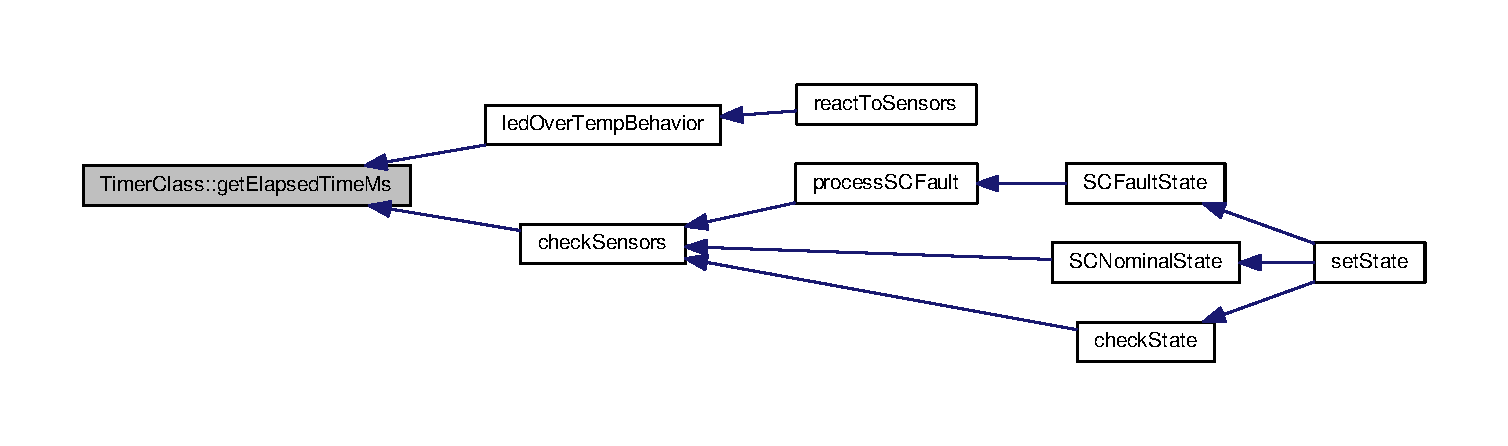
\includegraphics[width=350pt]{classTimerClass_ad989f6419974f0519f1d46419e9b5472_icgraph}
\end{center}
\end{figure}


\index{Timer\+Class@{Timer\+Class}!reset\+Timer@{reset\+Timer}}
\index{reset\+Timer@{reset\+Timer}!Timer\+Class@{Timer\+Class}}
\subsubsection[{\texorpdfstring{reset\+Timer(void)}{resetTimer(void)}}]{\setlength{\rightskip}{0pt plus 5cm}void Timer\+Class\+::reset\+Timer (
\begin{DoxyParamCaption}
\item[{void}]{}
\end{DoxyParamCaption}
)}\hypertarget{classTimerClass_a936be93f45ffb4a64d5d1b30552780cb}{}\label{classTimerClass_a936be93f45ffb4a64d5d1b30552780cb}


Here is the caller graph for this function\+:
\nopagebreak
\begin{figure}[H]
\begin{center}
\leavevmode
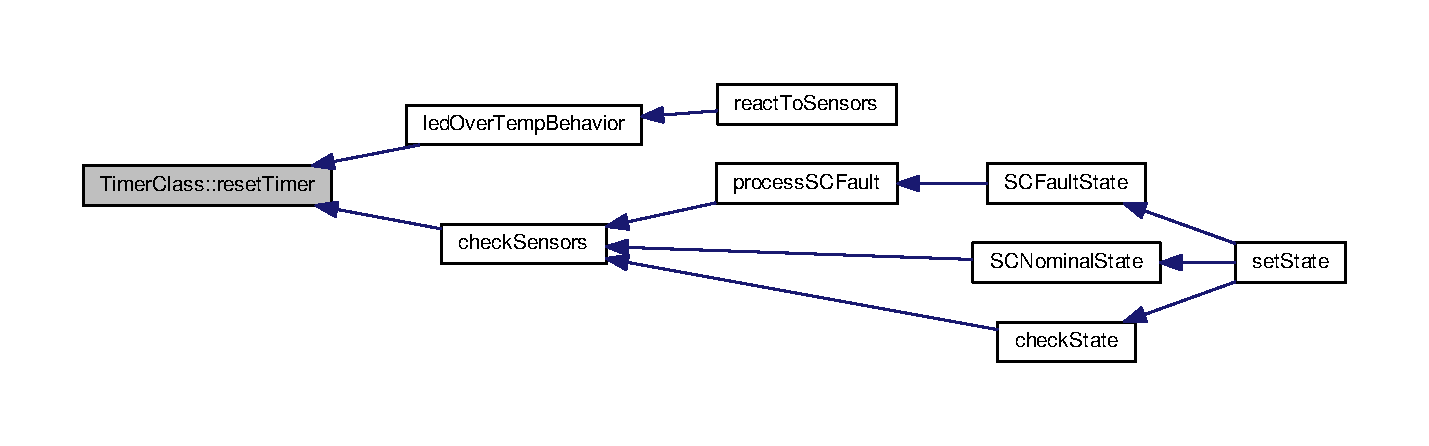
\includegraphics[width=350pt]{classTimerClass_a936be93f45ffb4a64d5d1b30552780cb_icgraph}
\end{center}
\end{figure}


\index{Timer\+Class@{Timer\+Class}!start\+Timer@{start\+Timer}}
\index{start\+Timer@{start\+Timer}!Timer\+Class@{Timer\+Class}}
\subsubsection[{\texorpdfstring{start\+Timer(void)}{startTimer(void)}}]{\setlength{\rightskip}{0pt plus 5cm}void Timer\+Class\+::start\+Timer (
\begin{DoxyParamCaption}
\item[{void}]{}
\end{DoxyParamCaption}
)}\hypertarget{classTimerClass_af40274762682bc80b9ec49fa54e0d5f3}{}\label{classTimerClass_af40274762682bc80b9ec49fa54e0d5f3}


Here is the caller graph for this function\+:
\nopagebreak
\begin{figure}[H]
\begin{center}
\leavevmode
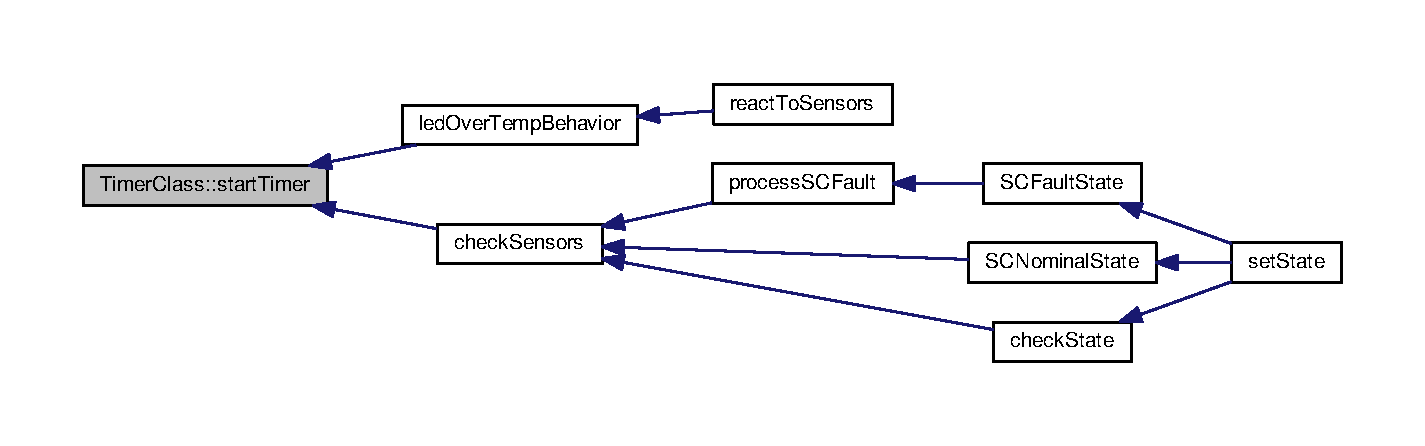
\includegraphics[width=350pt]{classTimerClass_af40274762682bc80b9ec49fa54e0d5f3_icgraph}
\end{center}
\end{figure}


\index{Timer\+Class@{Timer\+Class}!stop\+Timer@{stop\+Timer}}
\index{stop\+Timer@{stop\+Timer}!Timer\+Class@{Timer\+Class}}
\subsubsection[{\texorpdfstring{stop\+Timer(void)}{stopTimer(void)}}]{\setlength{\rightskip}{0pt plus 5cm}void Timer\+Class\+::stop\+Timer (
\begin{DoxyParamCaption}
\item[{void}]{}
\end{DoxyParamCaption}
)}\hypertarget{classTimerClass_a8feed88082813446d42a26e80a3e6f1a}{}\label{classTimerClass_a8feed88082813446d42a26e80a3e6f1a}


Here is the caller graph for this function\+:
\nopagebreak
\begin{figure}[H]
\begin{center}
\leavevmode
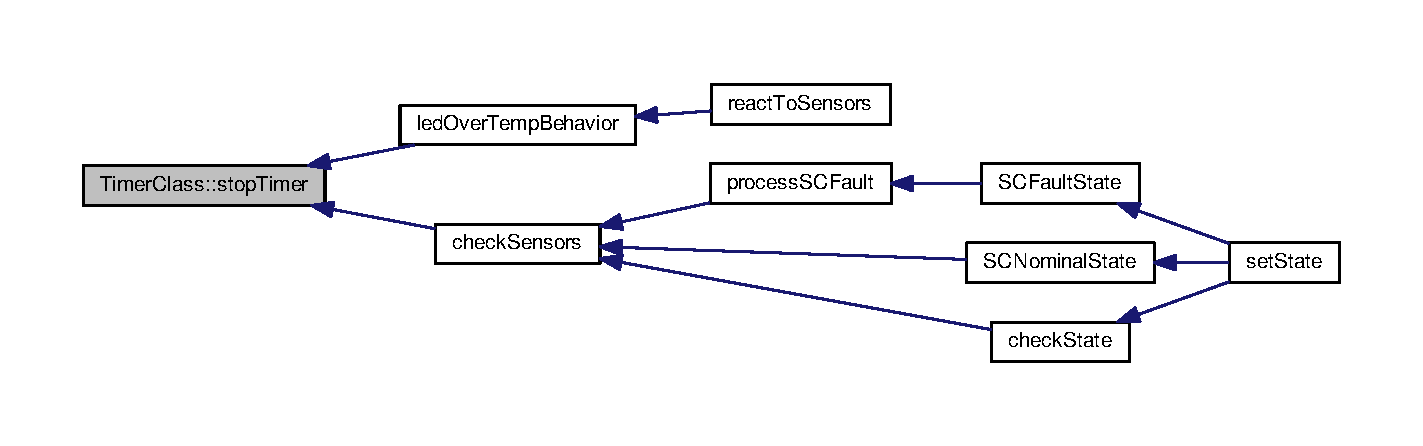
\includegraphics[width=350pt]{classTimerClass_a8feed88082813446d42a26e80a3e6f1a_icgraph}
\end{center}
\end{figure}




\subsection{Member Data Documentation}
\index{Timer\+Class@{Timer\+Class}!time\+Out\+Ms@{time\+Out\+Ms}}
\index{time\+Out\+Ms@{time\+Out\+Ms}!Timer\+Class@{Timer\+Class}}
\subsubsection[{\texorpdfstring{time\+Out\+Ms}{timeOutMs}}]{\setlength{\rightskip}{0pt plus 5cm}unsigned long Timer\+Class\+::time\+Out\+Ms}\hypertarget{classTimerClass_af5618246c8a06a9e0ff2b1c11deac3da}{}\label{classTimerClass_af5618246c8a06a9e0ff2b1c11deac3da}


The documentation for this class was generated from the following files\+:\begin{DoxyCompactItemize}
\item 
\hyperlink{Globals_8h}{Globals.\+h}\item 
\hyperlink{Globals_8cpp}{Globals.\+cpp}\end{DoxyCompactItemize}

\chapter{File Documentation}
\hypertarget{FaultHandler_8cpp}{}\section{Fault\+Handler.\+cpp File Reference}
\label{FaultHandler_8cpp}\index{Fault\+Handler.\+cpp@{Fault\+Handler.\+cpp}}
{\ttfamily \#include \char`\"{}Fault\+Handler.\+h\char`\"{}}\\*
{\ttfamily \#include \char`\"{}Globals.\+h\char`\"{}}\\*
{\ttfamily \#include \char`\"{}Sensor\+Manager.\+h\char`\"{}}\\*
Include dependency graph for Fault\+Handler.\+cpp\+:
\nopagebreak
\begin{figure}[H]
\begin{center}
\leavevmode
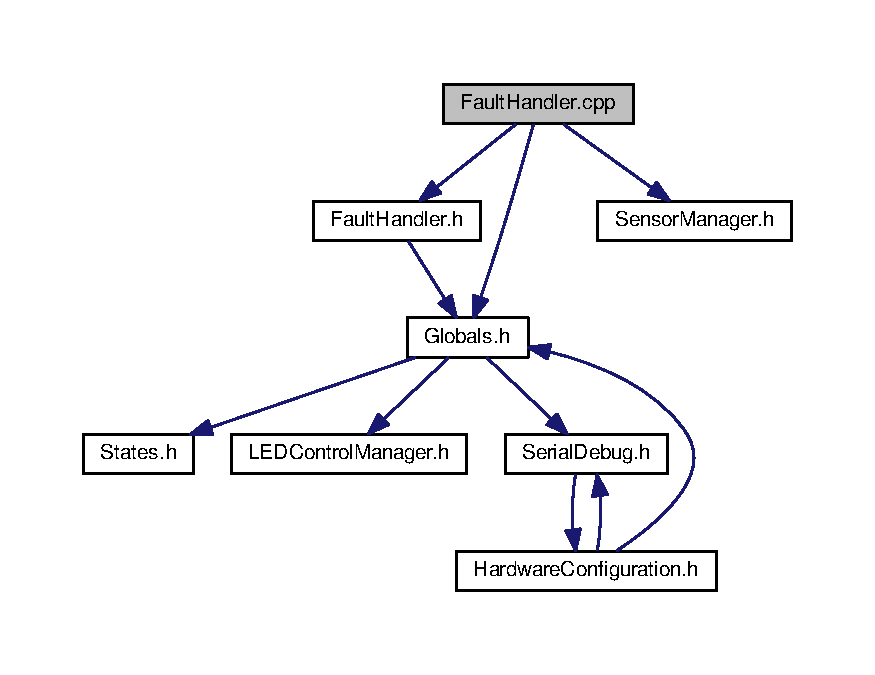
\includegraphics[width=350pt]{FaultHandler_8cpp__incl}
\end{center}
\end{figure}
\subsection*{Functions}
\begin{DoxyCompactItemize}
\item 
void \hyperlink{FaultHandler_8cpp_ae16fac85dbd867f57af7f50349a69cbe}{process\+S\+C\+Fault} (void)
\item 
void \hyperlink{FaultHandler_8cpp_aa59f3ab77e7e3c866bdc513d9925f93d}{process\+R\+G\+B\+Fault} (void)
\item 
void \hyperlink{FaultHandler_8cpp_ac8de8a862ca93b2dd5584982cce2d5a2}{led\+Over\+Temp\+Behavior} (void)
\item 
void \hyperlink{FaultHandler_8cpp_af7ed7ed53fb02033684a7bd77ce6864d}{input\+Voltage\+Error\+Behavior} (void)
\item 
void \hyperlink{FaultHandler_8cpp_a4e21fbf1ef6493f7765a365fa0ff62dd}{react\+To\+Sensors} (void)
\end{DoxyCompactItemize}
\subsection*{Variables}
\begin{DoxyCompactItemize}
\item 
class \hyperlink{classTimerClass}{Timer\+Class} \hyperlink{FaultHandler_8cpp_ac195cc1850a1f4575b7453b028c6fe01}{Voltage\+Timer}
\item 
class \hyperlink{classTimerClass}{Timer\+Class} \hyperlink{FaultHandler_8cpp_aed9c64591d033ba6765ec55e91c8ccf5}{Temp\+Error\+Timer}
\end{DoxyCompactItemize}


\subsection{Function Documentation}
\index{Fault\+Handler.\+cpp@{Fault\+Handler.\+cpp}!input\+Voltage\+Error\+Behavior@{input\+Voltage\+Error\+Behavior}}
\index{input\+Voltage\+Error\+Behavior@{input\+Voltage\+Error\+Behavior}!Fault\+Handler.\+cpp@{Fault\+Handler.\+cpp}}
\subsubsection[{\texorpdfstring{input\+Voltage\+Error\+Behavior(void)}{inputVoltageErrorBehavior(void)}}]{\setlength{\rightskip}{0pt plus 5cm}void input\+Voltage\+Error\+Behavior (
\begin{DoxyParamCaption}
\item[{void}]{}
\end{DoxyParamCaption}
)}\hypertarget{FaultHandler_8cpp_af7ed7ed53fb02033684a7bd77ce6864d}{}\label{FaultHandler_8cpp_af7ed7ed53fb02033684a7bd77ce6864d}


Here is the caller graph for this function\+:
\nopagebreak
\begin{figure}[H]
\begin{center}
\leavevmode
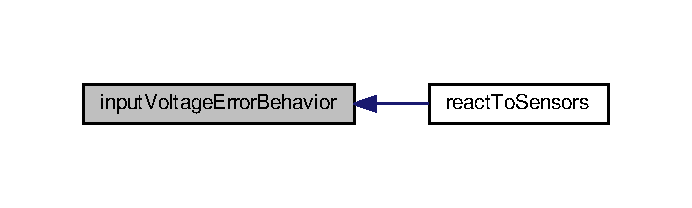
\includegraphics[width=332pt]{FaultHandler_8cpp_af7ed7ed53fb02033684a7bd77ce6864d_icgraph}
\end{center}
\end{figure}


\index{Fault\+Handler.\+cpp@{Fault\+Handler.\+cpp}!led\+Over\+Temp\+Behavior@{led\+Over\+Temp\+Behavior}}
\index{led\+Over\+Temp\+Behavior@{led\+Over\+Temp\+Behavior}!Fault\+Handler.\+cpp@{Fault\+Handler.\+cpp}}
\subsubsection[{\texorpdfstring{led\+Over\+Temp\+Behavior(void)}{ledOverTempBehavior(void)}}]{\setlength{\rightskip}{0pt plus 5cm}void led\+Over\+Temp\+Behavior (
\begin{DoxyParamCaption}
\item[{void}]{}
\end{DoxyParamCaption}
)}\hypertarget{FaultHandler_8cpp_ac8de8a862ca93b2dd5584982cce2d5a2}{}\label{FaultHandler_8cpp_ac8de8a862ca93b2dd5584982cce2d5a2}


Here is the call graph for this function\+:
\nopagebreak
\begin{figure}[H]
\begin{center}
\leavevmode
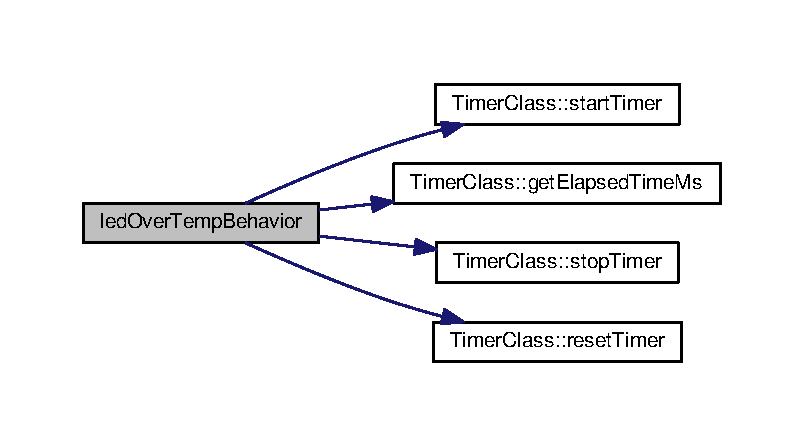
\includegraphics[width=350pt]{FaultHandler_8cpp_ac8de8a862ca93b2dd5584982cce2d5a2_cgraph}
\end{center}
\end{figure}




Here is the caller graph for this function\+:
\nopagebreak
\begin{figure}[H]
\begin{center}
\leavevmode
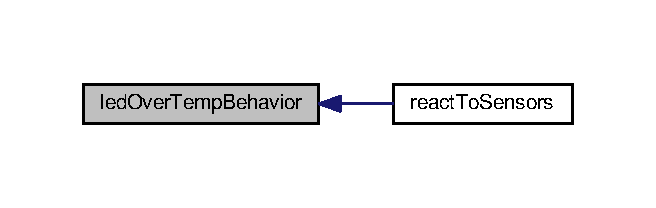
\includegraphics[width=315pt]{FaultHandler_8cpp_ac8de8a862ca93b2dd5584982cce2d5a2_icgraph}
\end{center}
\end{figure}


\index{Fault\+Handler.\+cpp@{Fault\+Handler.\+cpp}!process\+R\+G\+B\+Fault@{process\+R\+G\+B\+Fault}}
\index{process\+R\+G\+B\+Fault@{process\+R\+G\+B\+Fault}!Fault\+Handler.\+cpp@{Fault\+Handler.\+cpp}}
\subsubsection[{\texorpdfstring{process\+R\+G\+B\+Fault(void)}{processRGBFault(void)}}]{\setlength{\rightskip}{0pt plus 5cm}void process\+R\+G\+B\+Fault (
\begin{DoxyParamCaption}
\item[{void}]{}
\end{DoxyParamCaption}
)}\hypertarget{FaultHandler_8cpp_aa59f3ab77e7e3c866bdc513d9925f93d}{}\label{FaultHandler_8cpp_aa59f3ab77e7e3c866bdc513d9925f93d}
\index{Fault\+Handler.\+cpp@{Fault\+Handler.\+cpp}!process\+S\+C\+Fault@{process\+S\+C\+Fault}}
\index{process\+S\+C\+Fault@{process\+S\+C\+Fault}!Fault\+Handler.\+cpp@{Fault\+Handler.\+cpp}}
\subsubsection[{\texorpdfstring{process\+S\+C\+Fault(void)}{processSCFault(void)}}]{\setlength{\rightskip}{0pt plus 5cm}void process\+S\+C\+Fault (
\begin{DoxyParamCaption}
\item[{void}]{}
\end{DoxyParamCaption}
)}\hypertarget{FaultHandler_8cpp_ae16fac85dbd867f57af7f50349a69cbe}{}\label{FaultHandler_8cpp_ae16fac85dbd867f57af7f50349a69cbe}


Here is the call graph for this function\+:
\nopagebreak
\begin{figure}[H]
\begin{center}
\leavevmode
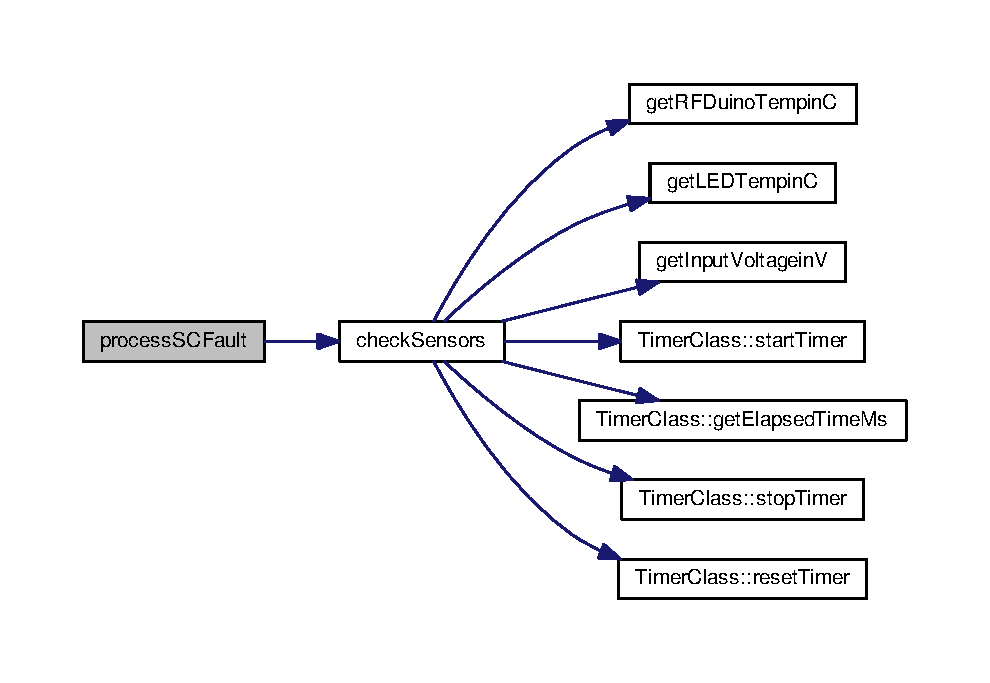
\includegraphics[width=350pt]{FaultHandler_8cpp_ae16fac85dbd867f57af7f50349a69cbe_cgraph}
\end{center}
\end{figure}




Here is the caller graph for this function\+:
\nopagebreak
\begin{figure}[H]
\begin{center}
\leavevmode
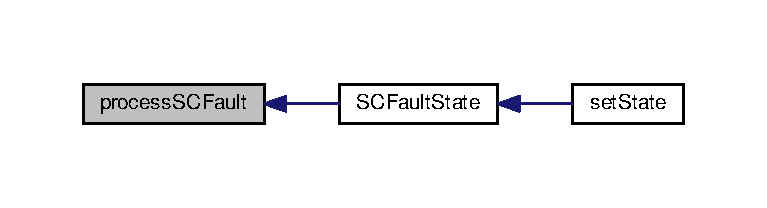
\includegraphics[width=350pt]{FaultHandler_8cpp_ae16fac85dbd867f57af7f50349a69cbe_icgraph}
\end{center}
\end{figure}


\index{Fault\+Handler.\+cpp@{Fault\+Handler.\+cpp}!react\+To\+Sensors@{react\+To\+Sensors}}
\index{react\+To\+Sensors@{react\+To\+Sensors}!Fault\+Handler.\+cpp@{Fault\+Handler.\+cpp}}
\subsubsection[{\texorpdfstring{react\+To\+Sensors(void)}{reactToSensors(void)}}]{\setlength{\rightskip}{0pt plus 5cm}void react\+To\+Sensors (
\begin{DoxyParamCaption}
\item[{void}]{}
\end{DoxyParamCaption}
)}\hypertarget{FaultHandler_8cpp_a4e21fbf1ef6493f7765a365fa0ff62dd}{}\label{FaultHandler_8cpp_a4e21fbf1ef6493f7765a365fa0ff62dd}


Here is the call graph for this function\+:
\nopagebreak
\begin{figure}[H]
\begin{center}
\leavevmode
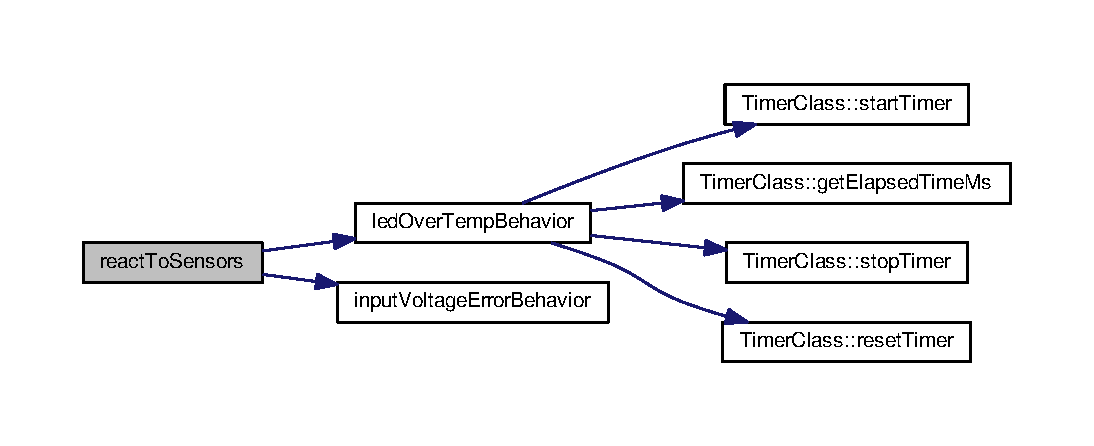
\includegraphics[width=350pt]{FaultHandler_8cpp_a4e21fbf1ef6493f7765a365fa0ff62dd_cgraph}
\end{center}
\end{figure}




\subsection{Variable Documentation}
\index{Fault\+Handler.\+cpp@{Fault\+Handler.\+cpp}!Temp\+Error\+Timer@{Temp\+Error\+Timer}}
\index{Temp\+Error\+Timer@{Temp\+Error\+Timer}!Fault\+Handler.\+cpp@{Fault\+Handler.\+cpp}}
\subsubsection[{\texorpdfstring{Temp\+Error\+Timer}{TempErrorTimer}}]{\setlength{\rightskip}{0pt plus 5cm}class {\bf Timer\+Class} Temp\+Error\+Timer}\hypertarget{FaultHandler_8cpp_aed9c64591d033ba6765ec55e91c8ccf5}{}\label{FaultHandler_8cpp_aed9c64591d033ba6765ec55e91c8ccf5}
\index{Fault\+Handler.\+cpp@{Fault\+Handler.\+cpp}!Voltage\+Timer@{Voltage\+Timer}}
\index{Voltage\+Timer@{Voltage\+Timer}!Fault\+Handler.\+cpp@{Fault\+Handler.\+cpp}}
\subsubsection[{\texorpdfstring{Voltage\+Timer}{VoltageTimer}}]{\setlength{\rightskip}{0pt plus 5cm}class {\bf Timer\+Class} Voltage\+Timer}\hypertarget{FaultHandler_8cpp_ac195cc1850a1f4575b7453b028c6fe01}{}\label{FaultHandler_8cpp_ac195cc1850a1f4575b7453b028c6fe01}

\hypertarget{FaultHandler_8h}{}\section{Fault\+Handler.\+h File Reference}
\label{FaultHandler_8h}\index{Fault\+Handler.\+h@{Fault\+Handler.\+h}}
{\ttfamily \#include \char`\"{}Globals.\+h\char`\"{}}\\*
Include dependency graph for Fault\+Handler.\+h\+:
\nopagebreak
\begin{figure}[H]
\begin{center}
\leavevmode
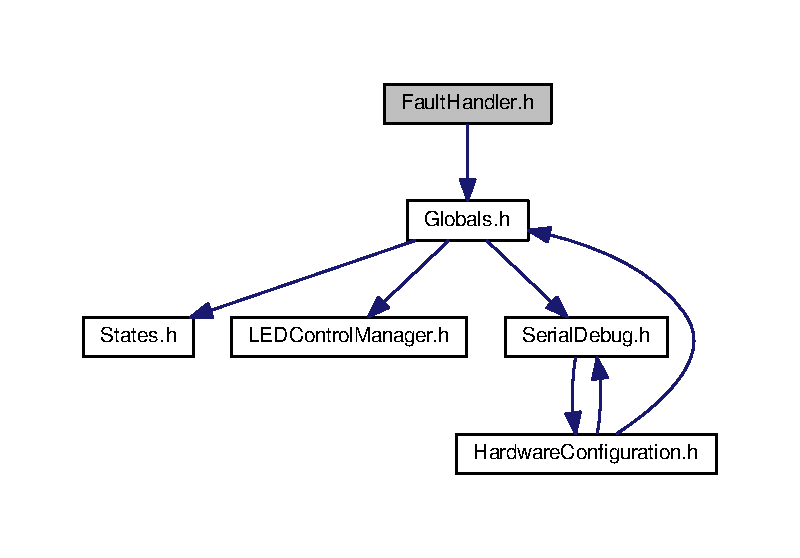
\includegraphics[width=350pt]{FaultHandler_8h__incl}
\end{center}
\end{figure}
This graph shows which files directly or indirectly include this file\+:
\nopagebreak
\begin{figure}[H]
\begin{center}
\leavevmode
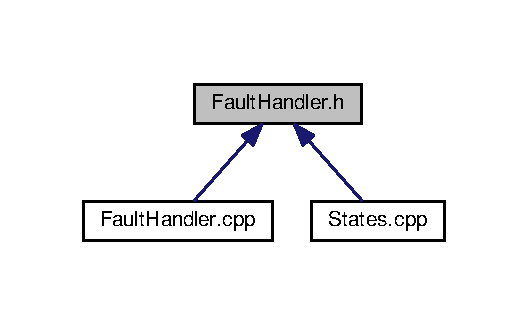
\includegraphics[width=253pt]{FaultHandler_8h__dep__incl}
\end{center}
\end{figure}
\subsection*{Macros}
\begin{DoxyCompactItemize}
\item 
\#define \hyperlink{FaultHandler_8h_af7cb00b3a3ae96e73aabf7045a8f143b}{L\+E\+D\+\_\+\+O\+V\+E\+R\+T\+E\+M\+P\+\_\+\+F\+I\+R\+S\+T\+\_\+\+R\+E\+D\+U\+C\+T\+I\+O\+N\+\_\+\+P\+E\+R\+C\+E\+N\+T\+A\+GE}~75
\end{DoxyCompactItemize}
\subsection*{Functions}
\begin{DoxyCompactItemize}
\item 
void \hyperlink{FaultHandler_8h_ae16fac85dbd867f57af7f50349a69cbe}{process\+S\+C\+Fault} (void)
\item 
void \hyperlink{FaultHandler_8h_aa59f3ab77e7e3c866bdc513d9925f93d}{process\+R\+G\+B\+Fault} (void)
\end{DoxyCompactItemize}


\subsection{Macro Definition Documentation}
\index{Fault\+Handler.\+h@{Fault\+Handler.\+h}!L\+E\+D\+\_\+\+O\+V\+E\+R\+T\+E\+M\+P\+\_\+\+F\+I\+R\+S\+T\+\_\+\+R\+E\+D\+U\+C\+T\+I\+O\+N\+\_\+\+P\+E\+R\+C\+E\+N\+T\+A\+GE@{L\+E\+D\+\_\+\+O\+V\+E\+R\+T\+E\+M\+P\+\_\+\+F\+I\+R\+S\+T\+\_\+\+R\+E\+D\+U\+C\+T\+I\+O\+N\+\_\+\+P\+E\+R\+C\+E\+N\+T\+A\+GE}}
\index{L\+E\+D\+\_\+\+O\+V\+E\+R\+T\+E\+M\+P\+\_\+\+F\+I\+R\+S\+T\+\_\+\+R\+E\+D\+U\+C\+T\+I\+O\+N\+\_\+\+P\+E\+R\+C\+E\+N\+T\+A\+GE@{L\+E\+D\+\_\+\+O\+V\+E\+R\+T\+E\+M\+P\+\_\+\+F\+I\+R\+S\+T\+\_\+\+R\+E\+D\+U\+C\+T\+I\+O\+N\+\_\+\+P\+E\+R\+C\+E\+N\+T\+A\+GE}!Fault\+Handler.\+h@{Fault\+Handler.\+h}}
\subsubsection[{\texorpdfstring{L\+E\+D\+\_\+\+O\+V\+E\+R\+T\+E\+M\+P\+\_\+\+F\+I\+R\+S\+T\+\_\+\+R\+E\+D\+U\+C\+T\+I\+O\+N\+\_\+\+P\+E\+R\+C\+E\+N\+T\+A\+GE}{LED_OVERTEMP_FIRST_REDUCTION_PERCENTAGE}}]{\setlength{\rightskip}{0pt plus 5cm}\#define L\+E\+D\+\_\+\+O\+V\+E\+R\+T\+E\+M\+P\+\_\+\+F\+I\+R\+S\+T\+\_\+\+R\+E\+D\+U\+C\+T\+I\+O\+N\+\_\+\+P\+E\+R\+C\+E\+N\+T\+A\+GE~75}\hypertarget{FaultHandler_8h_af7cb00b3a3ae96e73aabf7045a8f143b}{}\label{FaultHandler_8h_af7cb00b3a3ae96e73aabf7045a8f143b}


\subsection{Function Documentation}
\index{Fault\+Handler.\+h@{Fault\+Handler.\+h}!process\+R\+G\+B\+Fault@{process\+R\+G\+B\+Fault}}
\index{process\+R\+G\+B\+Fault@{process\+R\+G\+B\+Fault}!Fault\+Handler.\+h@{Fault\+Handler.\+h}}
\subsubsection[{\texorpdfstring{process\+R\+G\+B\+Fault(void)}{processRGBFault(void)}}]{\setlength{\rightskip}{0pt plus 5cm}void process\+R\+G\+B\+Fault (
\begin{DoxyParamCaption}
\item[{void}]{}
\end{DoxyParamCaption}
)}\hypertarget{FaultHandler_8h_aa59f3ab77e7e3c866bdc513d9925f93d}{}\label{FaultHandler_8h_aa59f3ab77e7e3c866bdc513d9925f93d}
\index{Fault\+Handler.\+h@{Fault\+Handler.\+h}!process\+S\+C\+Fault@{process\+S\+C\+Fault}}
\index{process\+S\+C\+Fault@{process\+S\+C\+Fault}!Fault\+Handler.\+h@{Fault\+Handler.\+h}}
\subsubsection[{\texorpdfstring{process\+S\+C\+Fault(void)}{processSCFault(void)}}]{\setlength{\rightskip}{0pt plus 5cm}void process\+S\+C\+Fault (
\begin{DoxyParamCaption}
\item[{void}]{}
\end{DoxyParamCaption}
)}\hypertarget{FaultHandler_8h_ae16fac85dbd867f57af7f50349a69cbe}{}\label{FaultHandler_8h_ae16fac85dbd867f57af7f50349a69cbe}


Here is the call graph for this function\+:
\nopagebreak
\begin{figure}[H]
\begin{center}
\leavevmode
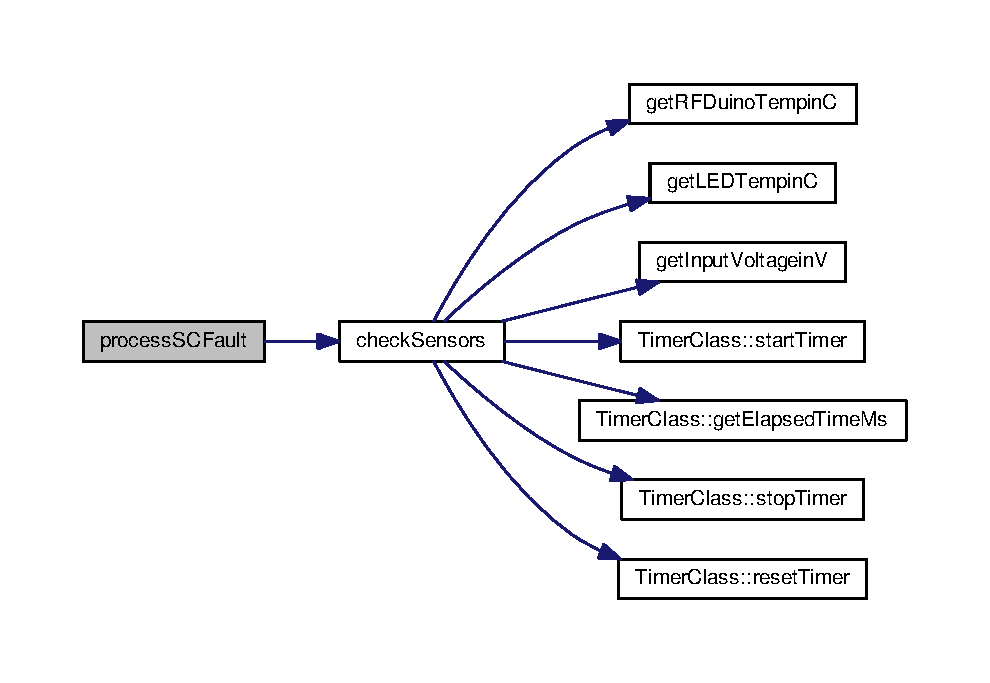
\includegraphics[width=350pt]{FaultHandler_8h_ae16fac85dbd867f57af7f50349a69cbe_cgraph}
\end{center}
\end{figure}




Here is the caller graph for this function\+:
\nopagebreak
\begin{figure}[H]
\begin{center}
\leavevmode
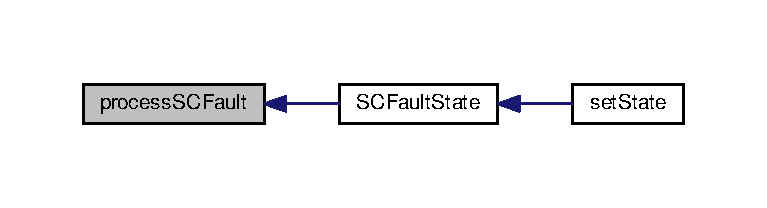
\includegraphics[width=350pt]{FaultHandler_8h_ae16fac85dbd867f57af7f50349a69cbe_icgraph}
\end{center}
\end{figure}



\hypertarget{Globals_8cpp}{}\section{Globals.\+cpp File Reference}
\label{Globals_8cpp}\index{Globals.\+cpp@{Globals.\+cpp}}
{\ttfamily \#include \char`\"{}Globals.\+h\char`\"{}}\\*
Include dependency graph for Globals.\+cpp\+:
\nopagebreak
\begin{figure}[H]
\begin{center}
\leavevmode
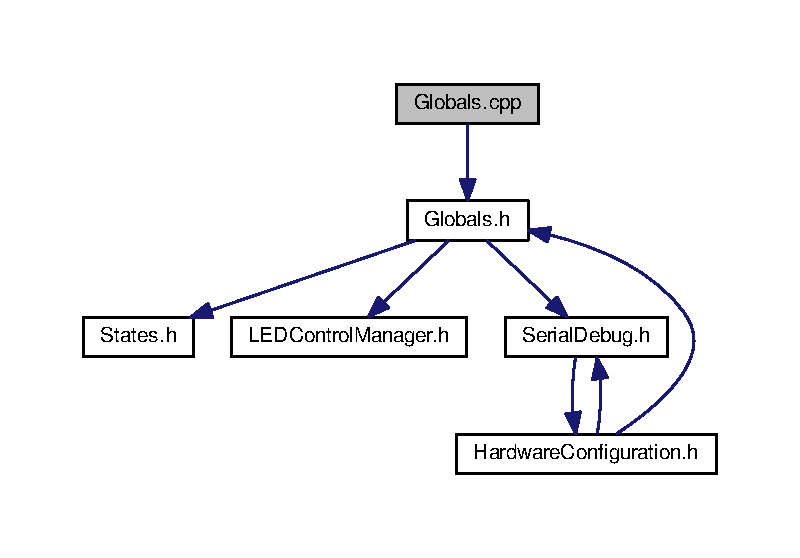
\includegraphics[width=350pt]{Globals_8cpp__incl}
\end{center}
\end{figure}
\subsection*{Functions}
\begin{DoxyCompactItemize}
\item 
void \hyperlink{Globals_8cpp_a2c5257cf1bf3583040988f1360b6ca4c}{load\+Flash\+Memory\+Values} (void)
\end{DoxyCompactItemize}
\subsection*{Variables}
\begin{DoxyCompactItemize}
\item 
unsigned long \hyperlink{Globals_8cpp_a8fb368eac6d1aa1a4402e31d3df91e20}{elapsed\+Time\+Ms} = 0
\item 
unsigned long \hyperlink{Globals_8cpp_a3e0d8b760ee641cc67bbf3e251a0f83d}{start\+Time\+Ms} = 0
\item 
unsigned long \hyperlink{Globals_8cpp_aabecee5a8e9e17fba895fe81cdd76f8f}{stop\+Time\+Ms} = 0
\item 
enum \hyperlink{States_8h_a808e5cd4979462d3bbe3070d7d147444}{States} \hyperlink{Globals_8cpp_aab6ab0beb9bba1649b7a760c93b4a235}{gbl\+\_\+system\+State} = \hyperlink{States_8h_a808e5cd4979462d3bbe3070d7d147444a1e36dd5b51c468e33bcf160523d402a7}{Boot}
\item 
bool \hyperlink{Globals_8cpp_abe3c2c1e6755cacc7b9ef7a8f9d9f9c7}{gbl\+\_\+system\+Boot\+Flag} = false
\item 
struct \hyperlink{structSCStatus}{S\+C\+Status} \hyperlink{Globals_8cpp_a81fbef388f3f2bc0df841916bcd0099c}{gbl\+\_\+\+S\+C\+Status} = \{0,false\}
\item 
unsigned long \hyperlink{Globals_8cpp_a354c49cca55c2b81a1cf4c4243706290}{gbl\+\_\+system\+Timerin\+Ms} = 0
\item 
struct \hyperlink{structFlashMemoryData}{Flash\+Memory\+Data} \hyperlink{Globals_8cpp_ae2343fcb262acdd3f1fc141578ea8d8a}{Flash\+Memory\+Data} = \{\}
\end{DoxyCompactItemize}


\subsection{Function Documentation}
\index{Globals.\+cpp@{Globals.\+cpp}!load\+Flash\+Memory\+Values@{load\+Flash\+Memory\+Values}}
\index{load\+Flash\+Memory\+Values@{load\+Flash\+Memory\+Values}!Globals.\+cpp@{Globals.\+cpp}}
\subsubsection[{\texorpdfstring{load\+Flash\+Memory\+Values(void)}{loadFlashMemoryValues(void)}}]{\setlength{\rightskip}{0pt plus 5cm}void load\+Flash\+Memory\+Values (
\begin{DoxyParamCaption}
\item[{void}]{}
\end{DoxyParamCaption}
)}\hypertarget{Globals_8cpp_a2c5257cf1bf3583040988f1360b6ca4c}{}\label{Globals_8cpp_a2c5257cf1bf3583040988f1360b6ca4c}


Here is the caller graph for this function\+:
\nopagebreak
\begin{figure}[H]
\begin{center}
\leavevmode
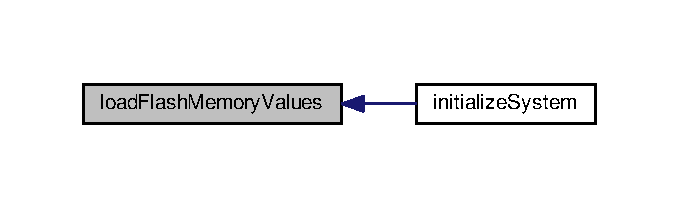
\includegraphics[width=326pt]{Globals_8cpp_a2c5257cf1bf3583040988f1360b6ca4c_icgraph}
\end{center}
\end{figure}




\subsection{Variable Documentation}
\index{Globals.\+cpp@{Globals.\+cpp}!elapsed\+Time\+Ms@{elapsed\+Time\+Ms}}
\index{elapsed\+Time\+Ms@{elapsed\+Time\+Ms}!Globals.\+cpp@{Globals.\+cpp}}
\subsubsection[{\texorpdfstring{elapsed\+Time\+Ms}{elapsedTimeMs}}]{\setlength{\rightskip}{0pt plus 5cm}unsigned long elapsed\+Time\+Ms = 0}\hypertarget{Globals_8cpp_a8fb368eac6d1aa1a4402e31d3df91e20}{}\label{Globals_8cpp_a8fb368eac6d1aa1a4402e31d3df91e20}
\index{Globals.\+cpp@{Globals.\+cpp}!Flash\+Memory\+Data@{Flash\+Memory\+Data}}
\index{Flash\+Memory\+Data@{Flash\+Memory\+Data}!Globals.\+cpp@{Globals.\+cpp}}
\subsubsection[{\texorpdfstring{Flash\+Memory\+Data}{FlashMemoryData}}]{\setlength{\rightskip}{0pt plus 5cm}struct {\bf Flash\+Memory\+Data} {\bf Flash\+Memory\+Data} = \{\}}\hypertarget{Globals_8cpp_ae2343fcb262acdd3f1fc141578ea8d8a}{}\label{Globals_8cpp_ae2343fcb262acdd3f1fc141578ea8d8a}
\index{Globals.\+cpp@{Globals.\+cpp}!gbl\+\_\+\+S\+C\+Status@{gbl\+\_\+\+S\+C\+Status}}
\index{gbl\+\_\+\+S\+C\+Status@{gbl\+\_\+\+S\+C\+Status}!Globals.\+cpp@{Globals.\+cpp}}
\subsubsection[{\texorpdfstring{gbl\+\_\+\+S\+C\+Status}{gbl_SCStatus}}]{\setlength{\rightskip}{0pt plus 5cm}struct {\bf S\+C\+Status} gbl\+\_\+\+S\+C\+Status = \{0,false\}}\hypertarget{Globals_8cpp_a81fbef388f3f2bc0df841916bcd0099c}{}\label{Globals_8cpp_a81fbef388f3f2bc0df841916bcd0099c}
\index{Globals.\+cpp@{Globals.\+cpp}!gbl\+\_\+system\+Boot\+Flag@{gbl\+\_\+system\+Boot\+Flag}}
\index{gbl\+\_\+system\+Boot\+Flag@{gbl\+\_\+system\+Boot\+Flag}!Globals.\+cpp@{Globals.\+cpp}}
\subsubsection[{\texorpdfstring{gbl\+\_\+system\+Boot\+Flag}{gbl_systemBootFlag}}]{\setlength{\rightskip}{0pt plus 5cm}bool gbl\+\_\+system\+Boot\+Flag = false}\hypertarget{Globals_8cpp_abe3c2c1e6755cacc7b9ef7a8f9d9f9c7}{}\label{Globals_8cpp_abe3c2c1e6755cacc7b9ef7a8f9d9f9c7}
\index{Globals.\+cpp@{Globals.\+cpp}!gbl\+\_\+system\+State@{gbl\+\_\+system\+State}}
\index{gbl\+\_\+system\+State@{gbl\+\_\+system\+State}!Globals.\+cpp@{Globals.\+cpp}}
\subsubsection[{\texorpdfstring{gbl\+\_\+system\+State}{gbl_systemState}}]{\setlength{\rightskip}{0pt plus 5cm}enum {\bf States} gbl\+\_\+system\+State = {\bf Boot}}\hypertarget{Globals_8cpp_aab6ab0beb9bba1649b7a760c93b4a235}{}\label{Globals_8cpp_aab6ab0beb9bba1649b7a760c93b4a235}
\index{Globals.\+cpp@{Globals.\+cpp}!gbl\+\_\+system\+Timerin\+Ms@{gbl\+\_\+system\+Timerin\+Ms}}
\index{gbl\+\_\+system\+Timerin\+Ms@{gbl\+\_\+system\+Timerin\+Ms}!Globals.\+cpp@{Globals.\+cpp}}
\subsubsection[{\texorpdfstring{gbl\+\_\+system\+Timerin\+Ms}{gbl_systemTimerinMs}}]{\setlength{\rightskip}{0pt plus 5cm}unsigned long gbl\+\_\+system\+Timerin\+Ms = 0}\hypertarget{Globals_8cpp_a354c49cca55c2b81a1cf4c4243706290}{}\label{Globals_8cpp_a354c49cca55c2b81a1cf4c4243706290}
\index{Globals.\+cpp@{Globals.\+cpp}!start\+Time\+Ms@{start\+Time\+Ms}}
\index{start\+Time\+Ms@{start\+Time\+Ms}!Globals.\+cpp@{Globals.\+cpp}}
\subsubsection[{\texorpdfstring{start\+Time\+Ms}{startTimeMs}}]{\setlength{\rightskip}{0pt plus 5cm}unsigned long start\+Time\+Ms = 0}\hypertarget{Globals_8cpp_a3e0d8b760ee641cc67bbf3e251a0f83d}{}\label{Globals_8cpp_a3e0d8b760ee641cc67bbf3e251a0f83d}
\index{Globals.\+cpp@{Globals.\+cpp}!stop\+Time\+Ms@{stop\+Time\+Ms}}
\index{stop\+Time\+Ms@{stop\+Time\+Ms}!Globals.\+cpp@{Globals.\+cpp}}
\subsubsection[{\texorpdfstring{stop\+Time\+Ms}{stopTimeMs}}]{\setlength{\rightskip}{0pt plus 5cm}unsigned long stop\+Time\+Ms = 0}\hypertarget{Globals_8cpp_aabecee5a8e9e17fba895fe81cdd76f8f}{}\label{Globals_8cpp_aabecee5a8e9e17fba895fe81cdd76f8f}

\hypertarget{Globals_8h}{}\section{Globals.\+h File Reference}
\label{Globals_8h}\index{Globals.\+h@{Globals.\+h}}
{\ttfamily \#include \char`\"{}States.\+h\char`\"{}}\\*
{\ttfamily \#include \char`\"{}L\+E\+D\+Control\+Manager.\+h\char`\"{}}\\*
{\ttfamily \#include \char`\"{}Serial\+Debug.\+h\char`\"{}}\\*
Include dependency graph for Globals.\+h\+:
\nopagebreak
\begin{figure}[H]
\begin{center}
\leavevmode
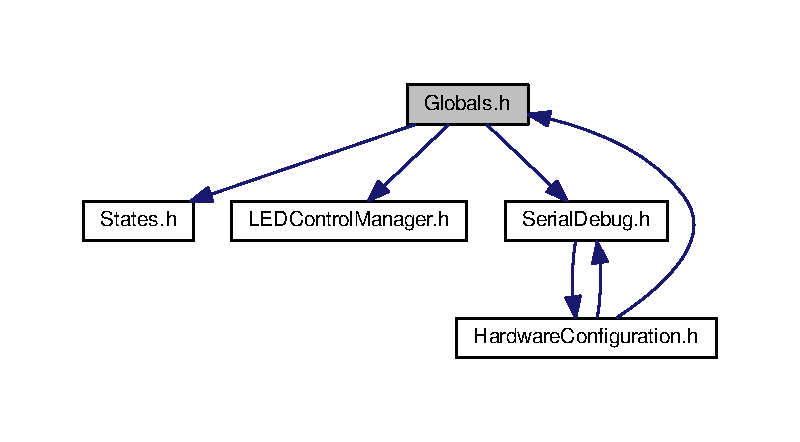
\includegraphics[width=350pt]{Globals_8h__incl}
\end{center}
\end{figure}
This graph shows which files directly or indirectly include this file\+:
\nopagebreak
\begin{figure}[H]
\begin{center}
\leavevmode
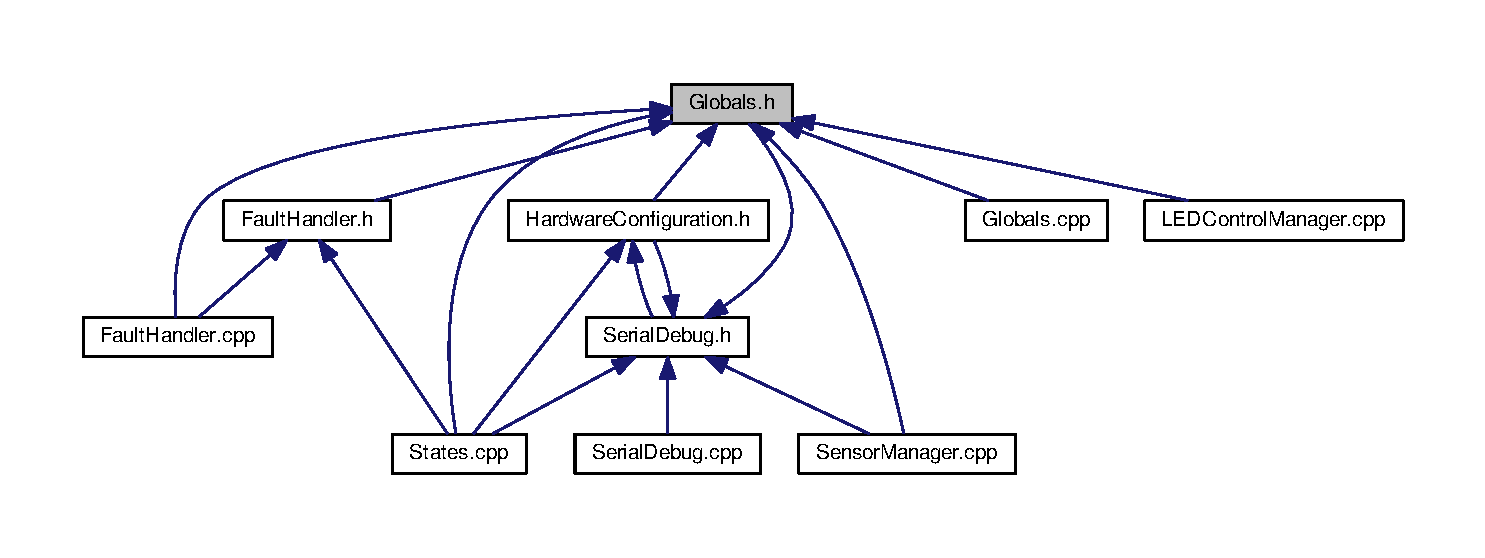
\includegraphics[width=350pt]{Globals_8h__dep__incl}
\end{center}
\end{figure}
\subsection*{Classes}
\begin{DoxyCompactItemize}
\item 
class \hyperlink{classTimerClass}{Timer\+Class}
\item 
struct \hyperlink{structFlashMemoryData}{Flash\+Memory\+Data}
\item 
struct \hyperlink{structSCStatus}{S\+C\+Status}
\end{DoxyCompactItemize}
\subsection*{Functions}
\begin{DoxyCompactItemize}
\item 
void \hyperlink{Globals_8h_a2c5257cf1bf3583040988f1360b6ca4c}{load\+Flash\+Memory\+Values} (void)
\item 
void \hyperlink{Globals_8h_adcd6dc41d959bb7cc02eb8856537aef2}{write\+New\+Timeof\+Use\+To\+Flash} (void)
\item 
void \hyperlink{Globals_8h_a8b8d2090e4025d1e0883a7a705d01eb0}{write\+All\+Settings\+To\+Flash} (void)
\end{DoxyCompactItemize}
\subsection*{Variables}
\begin{DoxyCompactItemize}
\item 
bool \hyperlink{Globals_8h_abe3c2c1e6755cacc7b9ef7a8f9d9f9c7}{gbl\+\_\+system\+Boot\+Flag}
\item 
struct \hyperlink{structSCStatus}{S\+C\+Status} \hyperlink{Globals_8h_a81fbef388f3f2bc0df841916bcd0099c}{gbl\+\_\+\+S\+C\+Status}
\item 
enum \hyperlink{States_8h_a808e5cd4979462d3bbe3070d7d147444}{States} \hyperlink{Globals_8h_aab6ab0beb9bba1649b7a760c93b4a235}{gbl\+\_\+system\+State}
\item 
struct \hyperlink{structFlashMemoryData}{Flash\+Memory\+Data} \hyperlink{Globals_8h_ae2343fcb262acdd3f1fc141578ea8d8a}{Flash\+Memory\+Data}
\item 
unsigned long \hyperlink{Globals_8h_a354c49cca55c2b81a1cf4c4243706290}{gbl\+\_\+system\+Timerin\+Ms}
\end{DoxyCompactItemize}


\subsection{Function Documentation}
\index{Globals.\+h@{Globals.\+h}!load\+Flash\+Memory\+Values@{load\+Flash\+Memory\+Values}}
\index{load\+Flash\+Memory\+Values@{load\+Flash\+Memory\+Values}!Globals.\+h@{Globals.\+h}}
\subsubsection[{\texorpdfstring{load\+Flash\+Memory\+Values(void)}{loadFlashMemoryValues(void)}}]{\setlength{\rightskip}{0pt plus 5cm}void load\+Flash\+Memory\+Values (
\begin{DoxyParamCaption}
\item[{void}]{}
\end{DoxyParamCaption}
)}\hypertarget{Globals_8h_a2c5257cf1bf3583040988f1360b6ca4c}{}\label{Globals_8h_a2c5257cf1bf3583040988f1360b6ca4c}


Here is the caller graph for this function\+:
\nopagebreak
\begin{figure}[H]
\begin{center}
\leavevmode
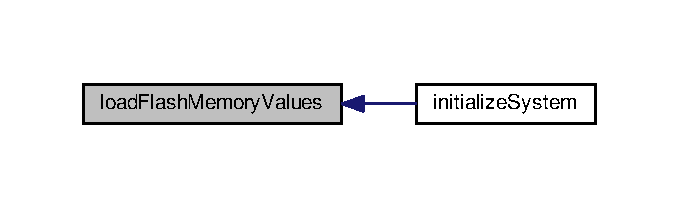
\includegraphics[width=326pt]{Globals_8h_a2c5257cf1bf3583040988f1360b6ca4c_icgraph}
\end{center}
\end{figure}


\index{Globals.\+h@{Globals.\+h}!write\+All\+Settings\+To\+Flash@{write\+All\+Settings\+To\+Flash}}
\index{write\+All\+Settings\+To\+Flash@{write\+All\+Settings\+To\+Flash}!Globals.\+h@{Globals.\+h}}
\subsubsection[{\texorpdfstring{write\+All\+Settings\+To\+Flash(void)}{writeAllSettingsToFlash(void)}}]{\setlength{\rightskip}{0pt plus 5cm}void write\+All\+Settings\+To\+Flash (
\begin{DoxyParamCaption}
\item[{void}]{}
\end{DoxyParamCaption}
)}\hypertarget{Globals_8h_a8b8d2090e4025d1e0883a7a705d01eb0}{}\label{Globals_8h_a8b8d2090e4025d1e0883a7a705d01eb0}
\index{Globals.\+h@{Globals.\+h}!write\+New\+Timeof\+Use\+To\+Flash@{write\+New\+Timeof\+Use\+To\+Flash}}
\index{write\+New\+Timeof\+Use\+To\+Flash@{write\+New\+Timeof\+Use\+To\+Flash}!Globals.\+h@{Globals.\+h}}
\subsubsection[{\texorpdfstring{write\+New\+Timeof\+Use\+To\+Flash(void)}{writeNewTimeofUseToFlash(void)}}]{\setlength{\rightskip}{0pt plus 5cm}void write\+New\+Timeof\+Use\+To\+Flash (
\begin{DoxyParamCaption}
\item[{void}]{}
\end{DoxyParamCaption}
)}\hypertarget{Globals_8h_adcd6dc41d959bb7cc02eb8856537aef2}{}\label{Globals_8h_adcd6dc41d959bb7cc02eb8856537aef2}


\subsection{Variable Documentation}
\index{Globals.\+h@{Globals.\+h}!Flash\+Memory\+Data@{Flash\+Memory\+Data}}
\index{Flash\+Memory\+Data@{Flash\+Memory\+Data}!Globals.\+h@{Globals.\+h}}
\subsubsection[{\texorpdfstring{Flash\+Memory\+Data}{FlashMemoryData}}]{\setlength{\rightskip}{0pt plus 5cm}struct {\bf Flash\+Memory\+Data} {\bf Flash\+Memory\+Data}}\hypertarget{Globals_8h_ae2343fcb262acdd3f1fc141578ea8d8a}{}\label{Globals_8h_ae2343fcb262acdd3f1fc141578ea8d8a}
\index{Globals.\+h@{Globals.\+h}!gbl\+\_\+\+S\+C\+Status@{gbl\+\_\+\+S\+C\+Status}}
\index{gbl\+\_\+\+S\+C\+Status@{gbl\+\_\+\+S\+C\+Status}!Globals.\+h@{Globals.\+h}}
\subsubsection[{\texorpdfstring{gbl\+\_\+\+S\+C\+Status}{gbl_SCStatus}}]{\setlength{\rightskip}{0pt plus 5cm}struct {\bf S\+C\+Status} gbl\+\_\+\+S\+C\+Status}\hypertarget{Globals_8h_a81fbef388f3f2bc0df841916bcd0099c}{}\label{Globals_8h_a81fbef388f3f2bc0df841916bcd0099c}
\index{Globals.\+h@{Globals.\+h}!gbl\+\_\+system\+Boot\+Flag@{gbl\+\_\+system\+Boot\+Flag}}
\index{gbl\+\_\+system\+Boot\+Flag@{gbl\+\_\+system\+Boot\+Flag}!Globals.\+h@{Globals.\+h}}
\subsubsection[{\texorpdfstring{gbl\+\_\+system\+Boot\+Flag}{gbl_systemBootFlag}}]{\setlength{\rightskip}{0pt plus 5cm}bool gbl\+\_\+system\+Boot\+Flag}\hypertarget{Globals_8h_abe3c2c1e6755cacc7b9ef7a8f9d9f9c7}{}\label{Globals_8h_abe3c2c1e6755cacc7b9ef7a8f9d9f9c7}
\index{Globals.\+h@{Globals.\+h}!gbl\+\_\+system\+State@{gbl\+\_\+system\+State}}
\index{gbl\+\_\+system\+State@{gbl\+\_\+system\+State}!Globals.\+h@{Globals.\+h}}
\subsubsection[{\texorpdfstring{gbl\+\_\+system\+State}{gbl_systemState}}]{\setlength{\rightskip}{0pt plus 5cm}enum {\bf States} gbl\+\_\+system\+State}\hypertarget{Globals_8h_aab6ab0beb9bba1649b7a760c93b4a235}{}\label{Globals_8h_aab6ab0beb9bba1649b7a760c93b4a235}
\index{Globals.\+h@{Globals.\+h}!gbl\+\_\+system\+Timerin\+Ms@{gbl\+\_\+system\+Timerin\+Ms}}
\index{gbl\+\_\+system\+Timerin\+Ms@{gbl\+\_\+system\+Timerin\+Ms}!Globals.\+h@{Globals.\+h}}
\subsubsection[{\texorpdfstring{gbl\+\_\+system\+Timerin\+Ms}{gbl_systemTimerinMs}}]{\setlength{\rightskip}{0pt plus 5cm}unsigned long gbl\+\_\+system\+Timerin\+Ms}\hypertarget{Globals_8h_a354c49cca55c2b81a1cf4c4243706290}{}\label{Globals_8h_a354c49cca55c2b81a1cf4c4243706290}

\hypertarget{HardwareConfiguration_8h}{}\section{Hardware\+Configuration.\+h File Reference}
\label{HardwareConfiguration_8h}\index{Hardware\+Configuration.\+h@{Hardware\+Configuration.\+h}}
{\ttfamily \#include \char`\"{}Globals.\+h\char`\"{}}\\*
{\ttfamily \#include \char`\"{}Serial\+Debug.\+h\char`\"{}}\\*
Include dependency graph for Hardware\+Configuration.\+h\+:
\nopagebreak
\begin{figure}[H]
\begin{center}
\leavevmode
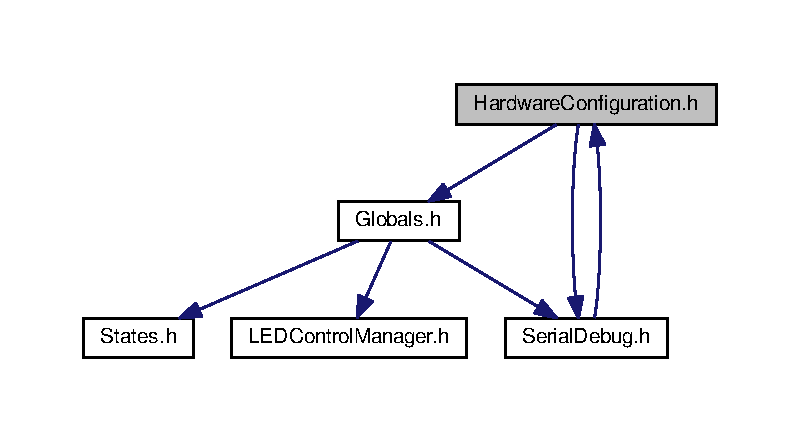
\includegraphics[width=350pt]{HardwareConfiguration_8h__incl}
\end{center}
\end{figure}
This graph shows which files directly or indirectly include this file\+:
\nopagebreak
\begin{figure}[H]
\begin{center}
\leavevmode
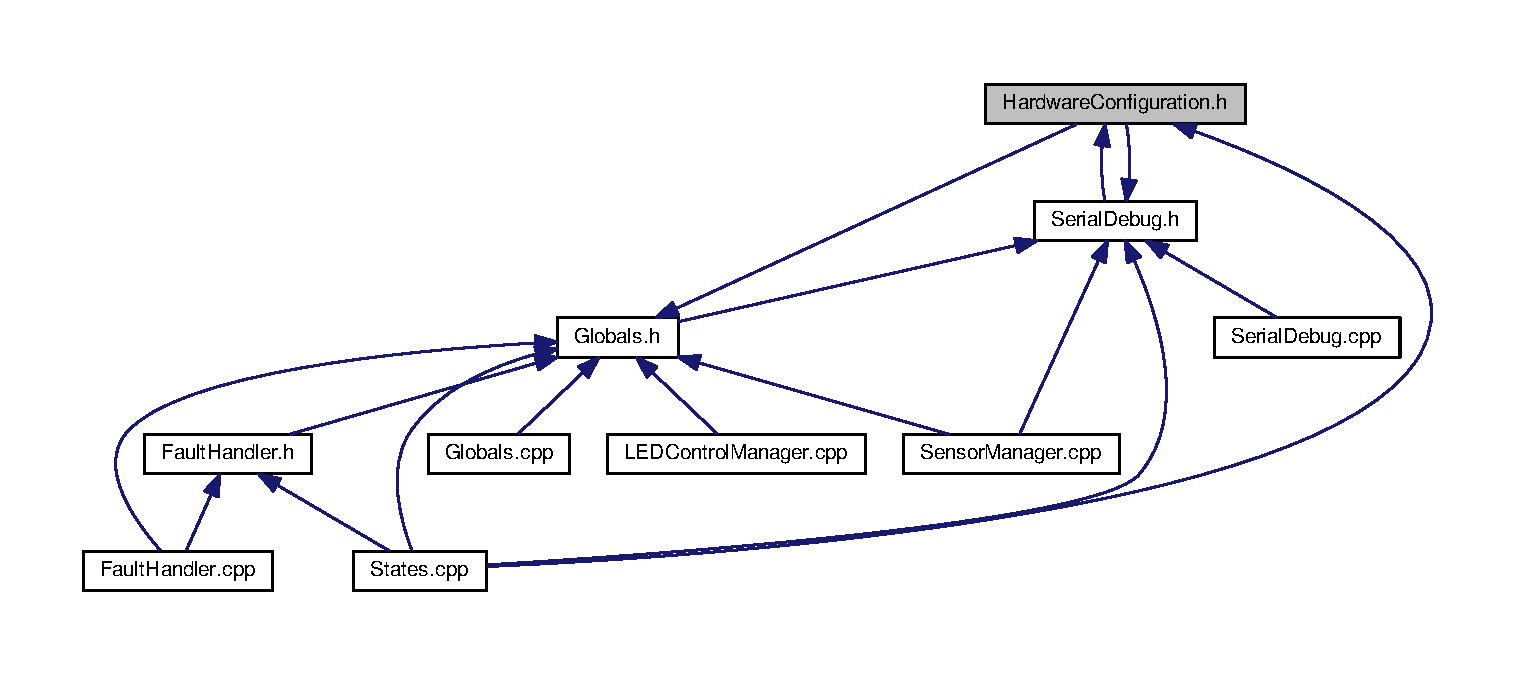
\includegraphics[width=350pt]{HardwareConfiguration_8h__dep__incl}
\end{center}
\end{figure}
\subsection*{Macros}
\begin{DoxyCompactItemize}
\item 
\#define \hyperlink{HardwareConfiguration_8h_a0da03efb4b5b70a36c8d72b0bb213a50}{S\+O\+F\+T\+W\+A\+R\+E\+\_\+\+V\+E\+R\+S\+I\+ON}~\char`\"{}0.\+0.\+0\char`\"{}
\item 
\#define \hyperlink{HardwareConfiguration_8h_a0923aeb0f386f79c74501a7406d09089}{R\+G\+B\+\_\+\+D\+R\+I\+V\+ER}~false
\item 
\#define \hyperlink{HardwareConfiguration_8h_a131ee562be22733e1593cad0beca210c}{R\+F\+\_\+\+T\+E\+L\+E\+M\+E\+T\+R\+Y\+\_\+\+E\+N\+A\+B\+L\+ED}~true
\item 
\#define \hyperlink{HardwareConfiguration_8h_afd709488633ade42ef9b5116738e30e3}{S\+E\+R\+I\+A\+L\+\_\+\+T\+E\+L\+E\+M\+E\+T\+R\+Y\+\_\+\+E\+N\+A\+B\+L\+ED}~true
\item 
\#define \hyperlink{HardwareConfiguration_8h_a5c9e262d97369ef158207d85c5c76571}{D\+E\+B\+U\+G\+\_\+\+R\+E\+F\+R\+E\+S\+H\+\_\+\+R\+A\+TE}~1000
\item 
\#define \hyperlink{HardwareConfiguration_8h_a4678d70a3e99dfd17be8df71c65fe626}{row1}~\char`\"{}    \+\_\+\+\_\+\+\_\+\+\_\+                    \+\_\+\+\_\+  \+\_\+\+\_\+                  \+\_\+\+\_\+\+\_\+\+\_\+\+\_\+\+\_\+                            \+\_\+\+\_\+\char`\"{}
\item 
\#define \hyperlink{HardwareConfiguration_8h_a65d4a12a1ff40ae74e8ac860271af6b9}{row2}~\char`\"{}   / \+\_\+\+\_\+ \textbackslash{}\textbackslash{}\+\_\+\+\_\+\+\_\+\+\_\+ \+\_\+\+\_\+\+\_\+  \+\_\+\+\_\+\+\_\+\+\_\+\+\_\+\+\_\+  / /\+\_\+/ /\+\_\+\+\_\+  \+\_\+\+\_\+\+\_\+\+\_\+\+\_\+\+\_\+\+\_\+\+\_\+\+\_\+\+\_\+   / \+\_\+\+\_\+\+\_\+\+\_\+/\+\_\+\+\_\+\+\_\+  \+\_\+\+\_\+\+\_\+\+\_\+  \+\_\+\+\_\+\+\_\+\+\_\+\+\_\+\+\_\+\+\_\+\+\_\+  \+\_\+\+\_\+\+\_\+\+\_\+  / /\+\_\+\+\_\+\+\_\+\+\_\+\+\_\+\+\_\+\char`\"{}
\item 
\#define \hyperlink{HardwareConfiguration_8h_ab5745acb2972907cb4742af68b508a02}{row3}~\char`\"{}  / / / / \+\_\+\+\_\+ `/ / / / \+\_\+\+\_\+ \textbackslash{}\textbackslash{}/ \+\_\+\+\_\+/ / \+\_\+ \textbackslash{}\textbackslash{}/ \+\_\+\+\_\+\+\_\+/ \+\_\+\+\_\+\+\_\+/  / /   / \+\_\+\+\_\+ \textbackslash{}\textbackslash{}/ \+\_\+\+\_\+ \textbackslash{}\textbackslash{}/ \+\_\+\+\_\+\+\_\+/ \+\_\+ \textbackslash{}\textbackslash{}/ \+\_\+\+\_\+ \textbackslash{}\textbackslash{}/ \+\_\+\+\_\+/ \+\_\+\+\_\+\+\_\+/\char`\"{}
\item 
\#define \hyperlink{HardwareConfiguration_8h_aee88dcc3f4ccc163bf9acfe022e56365}{row4}~\char`\"{} / /\+\_\+/ / /\+\_\+/ / /\+\_\+/ / / / / /\+\_\+/ /  \+\_\+\+\_\+(\+\_\+\+\_\+  $\vert$\+\_\+\+\_\+  )  / /\+\_\+\+\_\+\+\_\+/ /\+\_\+/ / / / / /\+\_\+\+\_\+/  \+\_\+\+\_\+/ /\+\_\+/ / /\+\_\+(\+\_\+\+\_\+  )\char`\"{}
\item 
\#define \hyperlink{HardwareConfiguration_8h_a0307cf1af67ffb843ffdfe2ca1e1938e}{row5}~\char`\"{}/\+\_\+\+\_\+\+\_\+\+\_\+\+\_\+/\textbackslash{}\textbackslash{}\+\_\+\+\_\+,\+\_\+/\textbackslash{}\textbackslash{}\+\_\+\+\_\+,\+\_\+/\+\_\+/ /\+\_\+/\textbackslash{}\textbackslash{}\+\_\+\+\_\+/\+\_\+/\textbackslash{}\textbackslash{}\+\_\+\+\_\+\+\_\+/\+\_\+\+\_\+\+\_\+\+\_\+/\+\_\+\+\_\+\+\_\+\+\_\+/   \textbackslash{}\textbackslash{}\+\_\+\+\_\+\+\_\+\+\_\+/\textbackslash{}\textbackslash{}\+\_\+\+\_\+\+\_\+\+\_\+/\+\_\+/ /\+\_\+/\textbackslash{}\textbackslash{}\+\_\+\+\_\+\+\_\+/\textbackslash{}\textbackslash{}\+\_\+\+\_\+\+\_\+/ .\+\_\+\+\_\+\+\_\+/\textbackslash{}\textbackslash{}\+\_\+\+\_\+/\+\_\+\+\_\+\+\_\+\+\_\+/\char`\"{}
\item 
\#define \hyperlink{HardwareConfiguration_8h_aae18083916baf008847ab77b7e822aa0}{row6}~\char`\"{}                                                                           /\+\_\+/\char`\"{}
\end{DoxyCompactItemize}


\subsection{Macro Definition Documentation}
\index{Hardware\+Configuration.\+h@{Hardware\+Configuration.\+h}!D\+E\+B\+U\+G\+\_\+\+R\+E\+F\+R\+E\+S\+H\+\_\+\+R\+A\+TE@{D\+E\+B\+U\+G\+\_\+\+R\+E\+F\+R\+E\+S\+H\+\_\+\+R\+A\+TE}}
\index{D\+E\+B\+U\+G\+\_\+\+R\+E\+F\+R\+E\+S\+H\+\_\+\+R\+A\+TE@{D\+E\+B\+U\+G\+\_\+\+R\+E\+F\+R\+E\+S\+H\+\_\+\+R\+A\+TE}!Hardware\+Configuration.\+h@{Hardware\+Configuration.\+h}}
\subsubsection[{\texorpdfstring{D\+E\+B\+U\+G\+\_\+\+R\+E\+F\+R\+E\+S\+H\+\_\+\+R\+A\+TE}{DEBUG_REFRESH_RATE}}]{\setlength{\rightskip}{0pt plus 5cm}\#define D\+E\+B\+U\+G\+\_\+\+R\+E\+F\+R\+E\+S\+H\+\_\+\+R\+A\+TE~1000}\hypertarget{HardwareConfiguration_8h_a5c9e262d97369ef158207d85c5c76571}{}\label{HardwareConfiguration_8h_a5c9e262d97369ef158207d85c5c76571}
\index{Hardware\+Configuration.\+h@{Hardware\+Configuration.\+h}!R\+F\+\_\+\+T\+E\+L\+E\+M\+E\+T\+R\+Y\+\_\+\+E\+N\+A\+B\+L\+ED@{R\+F\+\_\+\+T\+E\+L\+E\+M\+E\+T\+R\+Y\+\_\+\+E\+N\+A\+B\+L\+ED}}
\index{R\+F\+\_\+\+T\+E\+L\+E\+M\+E\+T\+R\+Y\+\_\+\+E\+N\+A\+B\+L\+ED@{R\+F\+\_\+\+T\+E\+L\+E\+M\+E\+T\+R\+Y\+\_\+\+E\+N\+A\+B\+L\+ED}!Hardware\+Configuration.\+h@{Hardware\+Configuration.\+h}}
\subsubsection[{\texorpdfstring{R\+F\+\_\+\+T\+E\+L\+E\+M\+E\+T\+R\+Y\+\_\+\+E\+N\+A\+B\+L\+ED}{RF_TELEMETRY_ENABLED}}]{\setlength{\rightskip}{0pt plus 5cm}\#define R\+F\+\_\+\+T\+E\+L\+E\+M\+E\+T\+R\+Y\+\_\+\+E\+N\+A\+B\+L\+ED~true}\hypertarget{HardwareConfiguration_8h_a131ee562be22733e1593cad0beca210c}{}\label{HardwareConfiguration_8h_a131ee562be22733e1593cad0beca210c}
\index{Hardware\+Configuration.\+h@{Hardware\+Configuration.\+h}!R\+G\+B\+\_\+\+D\+R\+I\+V\+ER@{R\+G\+B\+\_\+\+D\+R\+I\+V\+ER}}
\index{R\+G\+B\+\_\+\+D\+R\+I\+V\+ER@{R\+G\+B\+\_\+\+D\+R\+I\+V\+ER}!Hardware\+Configuration.\+h@{Hardware\+Configuration.\+h}}
\subsubsection[{\texorpdfstring{R\+G\+B\+\_\+\+D\+R\+I\+V\+ER}{RGB_DRIVER}}]{\setlength{\rightskip}{0pt plus 5cm}\#define R\+G\+B\+\_\+\+D\+R\+I\+V\+ER~false}\hypertarget{HardwareConfiguration_8h_a0923aeb0f386f79c74501a7406d09089}{}\label{HardwareConfiguration_8h_a0923aeb0f386f79c74501a7406d09089}
\index{Hardware\+Configuration.\+h@{Hardware\+Configuration.\+h}!row1@{row1}}
\index{row1@{row1}!Hardware\+Configuration.\+h@{Hardware\+Configuration.\+h}}
\subsubsection[{\texorpdfstring{row1}{row1}}]{\setlength{\rightskip}{0pt plus 5cm}\#define row1~\char`\"{}    \+\_\+\+\_\+\+\_\+\+\_\+                    \+\_\+\+\_\+  \+\_\+\+\_\+                  \+\_\+\+\_\+\+\_\+\+\_\+\+\_\+\+\_\+                            \+\_\+\+\_\+\char`\"{}}\hypertarget{HardwareConfiguration_8h_a4678d70a3e99dfd17be8df71c65fe626}{}\label{HardwareConfiguration_8h_a4678d70a3e99dfd17be8df71c65fe626}
\index{Hardware\+Configuration.\+h@{Hardware\+Configuration.\+h}!row2@{row2}}
\index{row2@{row2}!Hardware\+Configuration.\+h@{Hardware\+Configuration.\+h}}
\subsubsection[{\texorpdfstring{row2}{row2}}]{\setlength{\rightskip}{0pt plus 5cm}\#define row2~\char`\"{}   / \+\_\+\+\_\+ \textbackslash{}\textbackslash{}\+\_\+\+\_\+\+\_\+\+\_\+ \+\_\+\+\_\+\+\_\+  \+\_\+\+\_\+\+\_\+\+\_\+\+\_\+\+\_\+  / /\+\_\+/ /\+\_\+\+\_\+  \+\_\+\+\_\+\+\_\+\+\_\+\+\_\+\+\_\+\+\_\+\+\_\+\+\_\+\+\_\+   / \+\_\+\+\_\+\+\_\+\+\_\+/\+\_\+\+\_\+\+\_\+  \+\_\+\+\_\+\+\_\+\+\_\+  \+\_\+\+\_\+\+\_\+\+\_\+\+\_\+\+\_\+\+\_\+\+\_\+  \+\_\+\+\_\+\+\_\+\+\_\+  / /\+\_\+\+\_\+\+\_\+\+\_\+\+\_\+\+\_\+\char`\"{}}\hypertarget{HardwareConfiguration_8h_a65d4a12a1ff40ae74e8ac860271af6b9}{}\label{HardwareConfiguration_8h_a65d4a12a1ff40ae74e8ac860271af6b9}
\index{Hardware\+Configuration.\+h@{Hardware\+Configuration.\+h}!row3@{row3}}
\index{row3@{row3}!Hardware\+Configuration.\+h@{Hardware\+Configuration.\+h}}
\subsubsection[{\texorpdfstring{row3}{row3}}]{\setlength{\rightskip}{0pt plus 5cm}\#define row3~\char`\"{}  / / / / \+\_\+\+\_\+ `/ / / / \+\_\+\+\_\+ \textbackslash{}\textbackslash{}/ \+\_\+\+\_\+/ / \+\_\+ \textbackslash{}\textbackslash{}/ \+\_\+\+\_\+\+\_\+/ \+\_\+\+\_\+\+\_\+/  / /   / \+\_\+\+\_\+ \textbackslash{}\textbackslash{}/ \+\_\+\+\_\+ \textbackslash{}\textbackslash{}/ \+\_\+\+\_\+\+\_\+/ \+\_\+ \textbackslash{}\textbackslash{}/ \+\_\+\+\_\+ \textbackslash{}\textbackslash{}/ \+\_\+\+\_\+/ \+\_\+\+\_\+\+\_\+/\char`\"{}}\hypertarget{HardwareConfiguration_8h_ab5745acb2972907cb4742af68b508a02}{}\label{HardwareConfiguration_8h_ab5745acb2972907cb4742af68b508a02}
\index{Hardware\+Configuration.\+h@{Hardware\+Configuration.\+h}!row4@{row4}}
\index{row4@{row4}!Hardware\+Configuration.\+h@{Hardware\+Configuration.\+h}}
\subsubsection[{\texorpdfstring{row4}{row4}}]{\setlength{\rightskip}{0pt plus 5cm}\#define row4~\char`\"{} / /\+\_\+/ / /\+\_\+/ / /\+\_\+/ / / / / /\+\_\+/ /  \+\_\+\+\_\+(\+\_\+\+\_\+  $\vert$\+\_\+\+\_\+  )  / /\+\_\+\+\_\+\+\_\+/ /\+\_\+/ / / / / /\+\_\+\+\_\+/  \+\_\+\+\_\+/ /\+\_\+/ / /\+\_\+(\+\_\+\+\_\+  )\char`\"{}}\hypertarget{HardwareConfiguration_8h_aee88dcc3f4ccc163bf9acfe022e56365}{}\label{HardwareConfiguration_8h_aee88dcc3f4ccc163bf9acfe022e56365}
\index{Hardware\+Configuration.\+h@{Hardware\+Configuration.\+h}!row5@{row5}}
\index{row5@{row5}!Hardware\+Configuration.\+h@{Hardware\+Configuration.\+h}}
\subsubsection[{\texorpdfstring{row5}{row5}}]{\setlength{\rightskip}{0pt plus 5cm}\#define row5~\char`\"{}/\+\_\+\+\_\+\+\_\+\+\_\+\+\_\+/\textbackslash{}\textbackslash{}\+\_\+\+\_\+,\+\_\+/\textbackslash{}\textbackslash{}\+\_\+\+\_\+,\+\_\+/\+\_\+/ /\+\_\+/\textbackslash{}\textbackslash{}\+\_\+\+\_\+/\+\_\+/\textbackslash{}\textbackslash{}\+\_\+\+\_\+\+\_\+/\+\_\+\+\_\+\+\_\+\+\_\+/\+\_\+\+\_\+\+\_\+\+\_\+/   \textbackslash{}\textbackslash{}\+\_\+\+\_\+\+\_\+\+\_\+/\textbackslash{}\textbackslash{}\+\_\+\+\_\+\+\_\+\+\_\+/\+\_\+/ /\+\_\+/\textbackslash{}\textbackslash{}\+\_\+\+\_\+\+\_\+/\textbackslash{}\textbackslash{}\+\_\+\+\_\+\+\_\+/ .\+\_\+\+\_\+\+\_\+/\textbackslash{}\textbackslash{}\+\_\+\+\_\+/\+\_\+\+\_\+\+\_\+\+\_\+/\char`\"{}}\hypertarget{HardwareConfiguration_8h_a0307cf1af67ffb843ffdfe2ca1e1938e}{}\label{HardwareConfiguration_8h_a0307cf1af67ffb843ffdfe2ca1e1938e}
\index{Hardware\+Configuration.\+h@{Hardware\+Configuration.\+h}!row6@{row6}}
\index{row6@{row6}!Hardware\+Configuration.\+h@{Hardware\+Configuration.\+h}}
\subsubsection[{\texorpdfstring{row6}{row6}}]{\setlength{\rightskip}{0pt plus 5cm}\#define row6~\char`\"{}                                                                           /\+\_\+/\char`\"{}}\hypertarget{HardwareConfiguration_8h_aae18083916baf008847ab77b7e822aa0}{}\label{HardwareConfiguration_8h_aae18083916baf008847ab77b7e822aa0}
\index{Hardware\+Configuration.\+h@{Hardware\+Configuration.\+h}!S\+E\+R\+I\+A\+L\+\_\+\+T\+E\+L\+E\+M\+E\+T\+R\+Y\+\_\+\+E\+N\+A\+B\+L\+ED@{S\+E\+R\+I\+A\+L\+\_\+\+T\+E\+L\+E\+M\+E\+T\+R\+Y\+\_\+\+E\+N\+A\+B\+L\+ED}}
\index{S\+E\+R\+I\+A\+L\+\_\+\+T\+E\+L\+E\+M\+E\+T\+R\+Y\+\_\+\+E\+N\+A\+B\+L\+ED@{S\+E\+R\+I\+A\+L\+\_\+\+T\+E\+L\+E\+M\+E\+T\+R\+Y\+\_\+\+E\+N\+A\+B\+L\+ED}!Hardware\+Configuration.\+h@{Hardware\+Configuration.\+h}}
\subsubsection[{\texorpdfstring{S\+E\+R\+I\+A\+L\+\_\+\+T\+E\+L\+E\+M\+E\+T\+R\+Y\+\_\+\+E\+N\+A\+B\+L\+ED}{SERIAL_TELEMETRY_ENABLED}}]{\setlength{\rightskip}{0pt plus 5cm}\#define S\+E\+R\+I\+A\+L\+\_\+\+T\+E\+L\+E\+M\+E\+T\+R\+Y\+\_\+\+E\+N\+A\+B\+L\+ED~true}\hypertarget{HardwareConfiguration_8h_afd709488633ade42ef9b5116738e30e3}{}\label{HardwareConfiguration_8h_afd709488633ade42ef9b5116738e30e3}
\index{Hardware\+Configuration.\+h@{Hardware\+Configuration.\+h}!S\+O\+F\+T\+W\+A\+R\+E\+\_\+\+V\+E\+R\+S\+I\+ON@{S\+O\+F\+T\+W\+A\+R\+E\+\_\+\+V\+E\+R\+S\+I\+ON}}
\index{S\+O\+F\+T\+W\+A\+R\+E\+\_\+\+V\+E\+R\+S\+I\+ON@{S\+O\+F\+T\+W\+A\+R\+E\+\_\+\+V\+E\+R\+S\+I\+ON}!Hardware\+Configuration.\+h@{Hardware\+Configuration.\+h}}
\subsubsection[{\texorpdfstring{S\+O\+F\+T\+W\+A\+R\+E\+\_\+\+V\+E\+R\+S\+I\+ON}{SOFTWARE_VERSION}}]{\setlength{\rightskip}{0pt plus 5cm}\#define S\+O\+F\+T\+W\+A\+R\+E\+\_\+\+V\+E\+R\+S\+I\+ON~\char`\"{}0.\+0.\+0\char`\"{}}\hypertarget{HardwareConfiguration_8h_a0da03efb4b5b70a36c8d72b0bb213a50}{}\label{HardwareConfiguration_8h_a0da03efb4b5b70a36c8d72b0bb213a50}

\hypertarget{LEDControlManager_8cpp}{}\section{L\+E\+D\+Control\+Manager.\+cpp File Reference}
\label{LEDControlManager_8cpp}\index{L\+E\+D\+Control\+Manager.\+cpp@{L\+E\+D\+Control\+Manager.\+cpp}}
{\ttfamily \#include \char`\"{}L\+E\+D\+Control\+Manager.\+h\char`\"{}}\\*
{\ttfamily \#include \char`\"{}Globals.\+h\char`\"{}}\\*
{\ttfamily \#include \char`\"{}Pin\+Definitions.\+h\char`\"{}}\\*
{\ttfamily \#include $<$Arduino.\+h$>$}\\*
Include dependency graph for L\+E\+D\+Control\+Manager.\+cpp\+:
\nopagebreak
\begin{figure}[H]
\begin{center}
\leavevmode
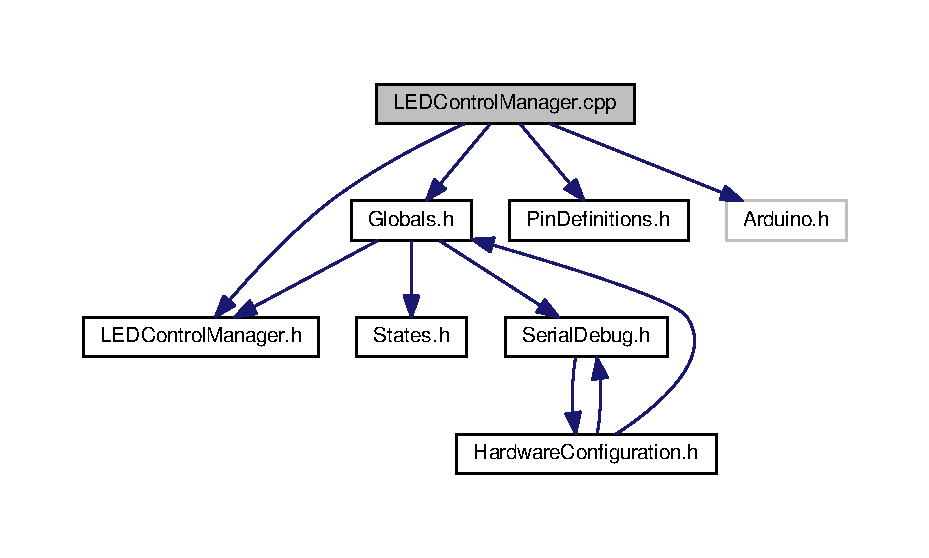
\includegraphics[width=350pt]{LEDControlManager_8cpp__incl}
\end{center}
\end{figure}
\subsection*{Functions}
\begin{DoxyCompactItemize}
\item 
void \hyperlink{LEDControlManager_8cpp_a44568cbb326ce94b800b1407bd74c3a3}{set\+Red\+P\+WM} (char percent)
\item 
void \hyperlink{LEDControlManager_8cpp_a1fb733347d7b1ebbae42b0078ede5453}{set\+S\+C\+Intensity} (void)
\end{DoxyCompactItemize}


\subsection{Function Documentation}
\index{L\+E\+D\+Control\+Manager.\+cpp@{L\+E\+D\+Control\+Manager.\+cpp}!set\+Red\+P\+WM@{set\+Red\+P\+WM}}
\index{set\+Red\+P\+WM@{set\+Red\+P\+WM}!L\+E\+D\+Control\+Manager.\+cpp@{L\+E\+D\+Control\+Manager.\+cpp}}
\subsubsection[{\texorpdfstring{set\+Red\+P\+W\+M(char percent)}{setRedPWM(char percent)}}]{\setlength{\rightskip}{0pt plus 5cm}void set\+Red\+P\+WM (
\begin{DoxyParamCaption}
\item[{char}]{percent}
\end{DoxyParamCaption}
)}\hypertarget{LEDControlManager_8cpp_a44568cbb326ce94b800b1407bd74c3a3}{}\label{LEDControlManager_8cpp_a44568cbb326ce94b800b1407bd74c3a3}


Here is the call graph for this function\+:
\nopagebreak
\begin{figure}[H]
\begin{center}
\leavevmode
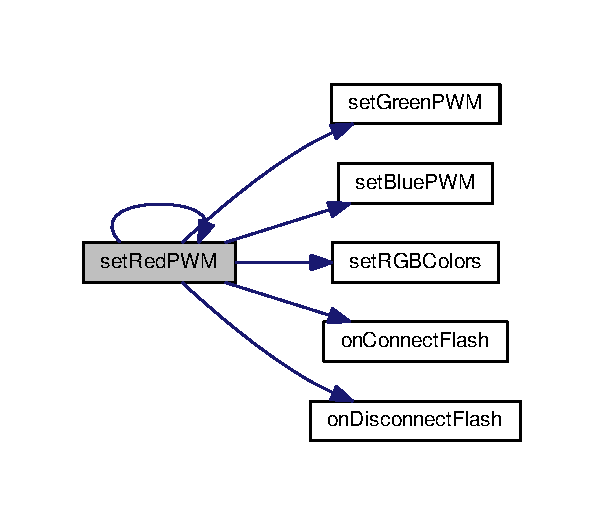
\includegraphics[width=290pt]{LEDControlManager_8cpp_a44568cbb326ce94b800b1407bd74c3a3_cgraph}
\end{center}
\end{figure}




Here is the caller graph for this function\+:
\nopagebreak
\begin{figure}[H]
\begin{center}
\leavevmode
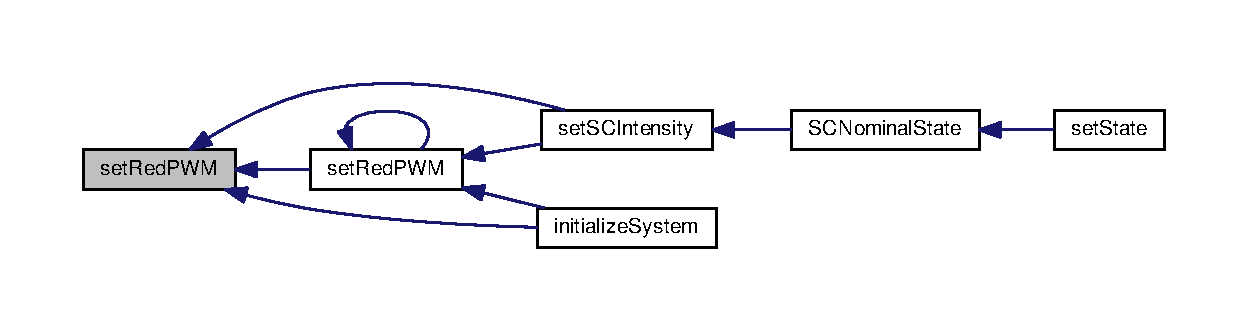
\includegraphics[width=350pt]{LEDControlManager_8cpp_a44568cbb326ce94b800b1407bd74c3a3_icgraph}
\end{center}
\end{figure}


\index{L\+E\+D\+Control\+Manager.\+cpp@{L\+E\+D\+Control\+Manager.\+cpp}!set\+S\+C\+Intensity@{set\+S\+C\+Intensity}}
\index{set\+S\+C\+Intensity@{set\+S\+C\+Intensity}!L\+E\+D\+Control\+Manager.\+cpp@{L\+E\+D\+Control\+Manager.\+cpp}}
\subsubsection[{\texorpdfstring{set\+S\+C\+Intensity(void)}{setSCIntensity(void)}}]{\setlength{\rightskip}{0pt plus 5cm}void set\+S\+C\+Intensity (
\begin{DoxyParamCaption}
\item[{void}]{}
\end{DoxyParamCaption}
)}\hypertarget{LEDControlManager_8cpp_a1fb733347d7b1ebbae42b0078ede5453}{}\label{LEDControlManager_8cpp_a1fb733347d7b1ebbae42b0078ede5453}


Here is the call graph for this function\+:
\nopagebreak
\begin{figure}[H]
\begin{center}
\leavevmode
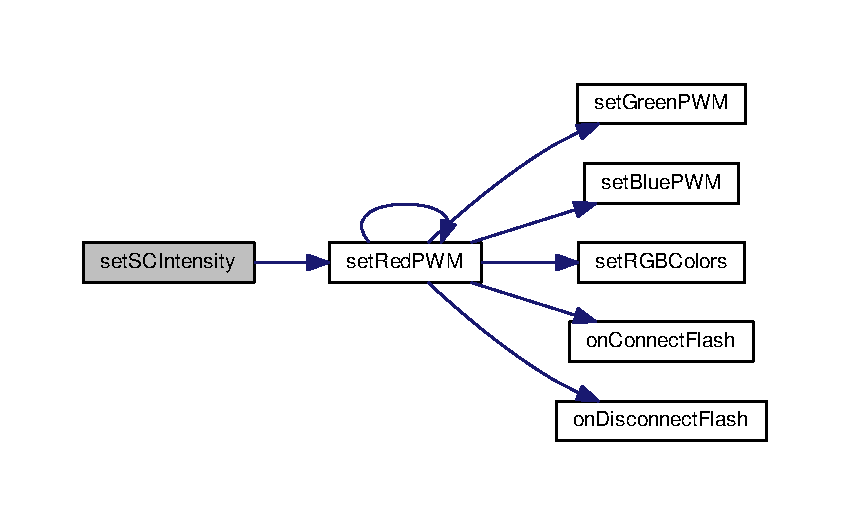
\includegraphics[width=350pt]{LEDControlManager_8cpp_a1fb733347d7b1ebbae42b0078ede5453_cgraph}
\end{center}
\end{figure}




Here is the caller graph for this function\+:
\nopagebreak
\begin{figure}[H]
\begin{center}
\leavevmode
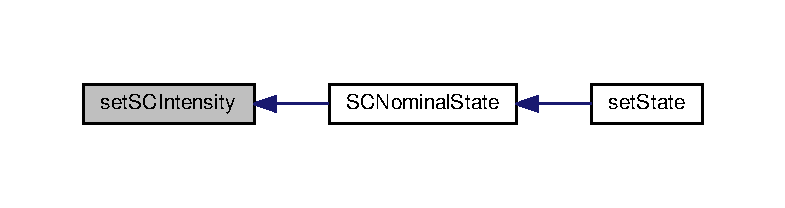
\includegraphics[width=350pt]{LEDControlManager_8cpp_a1fb733347d7b1ebbae42b0078ede5453_icgraph}
\end{center}
\end{figure}



\hypertarget{LEDControlManager_8h}{}\section{L\+E\+D\+Control\+Manager.\+h File Reference}
\label{LEDControlManager_8h}\index{L\+E\+D\+Control\+Manager.\+h@{L\+E\+D\+Control\+Manager.\+h}}
This graph shows which files directly or indirectly include this file\+:
\nopagebreak
\begin{figure}[H]
\begin{center}
\leavevmode
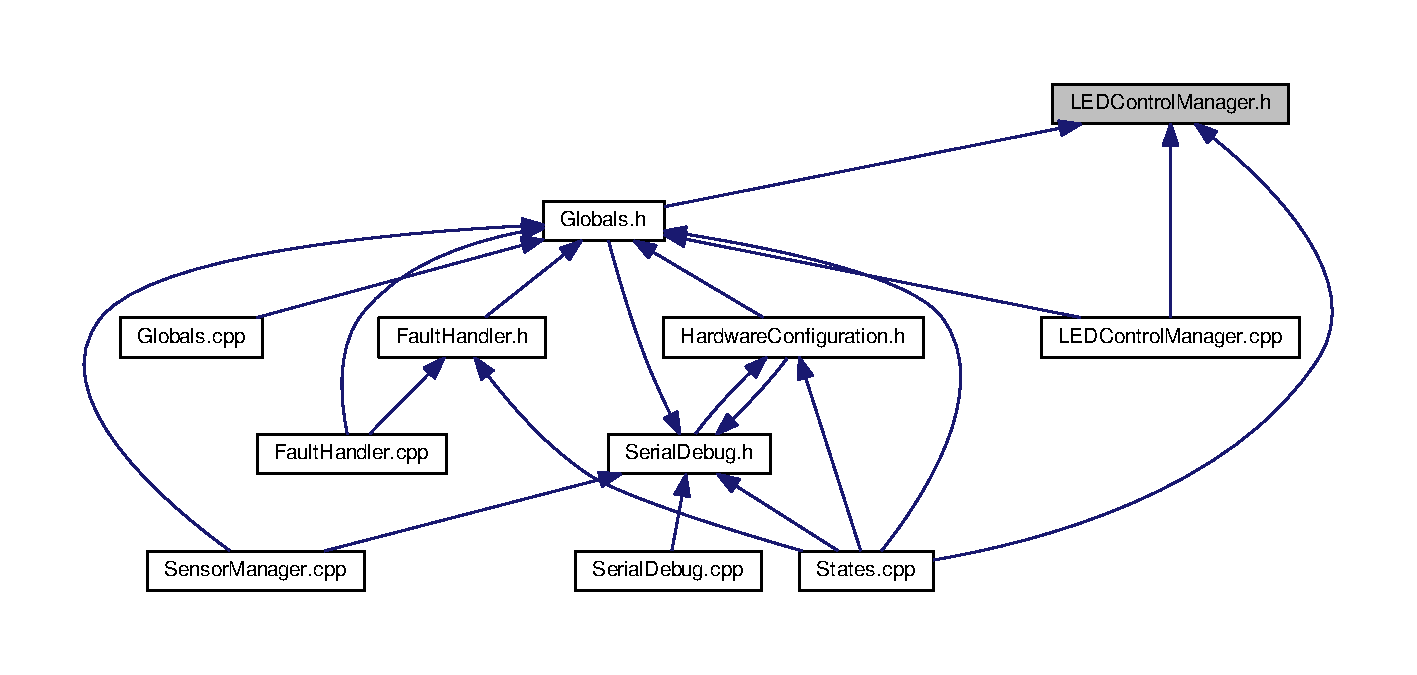
\includegraphics[width=350pt]{LEDControlManager_8h__dep__incl}
\end{center}
\end{figure}
\subsection*{Functions}
\begin{DoxyCompactItemize}
\item 
void \hyperlink{LEDControlManager_8h_a1fb733347d7b1ebbae42b0078ede5453}{set\+S\+C\+Intensity} (void)
\item 
void \hyperlink{LEDControlManager_8h_a44568cbb326ce94b800b1407bd74c3a3}{set\+Red\+P\+WM} (char percent)
\item 
void \hyperlink{LEDControlManager_8h_a5f7040b85d3431166dad2842730f077c}{set\+Green\+P\+WM} (char percent)
\item 
void \hyperlink{LEDControlManager_8h_a91457a286ce7ad9931a802f91dd1542c}{set\+Blue\+P\+WM} (char percent)
\item 
void \hyperlink{LEDControlManager_8h_a63e99d1d357e27cdba2122126293ac7a}{set\+R\+G\+B\+Colors} (void)
\item 
void \hyperlink{LEDControlManager_8h_ad3ec9b8ca1fb8ab67b960876b5761b42}{on\+Connect\+Flash} (void)
\item 
void \hyperlink{LEDControlManager_8h_a9e6967c01a7e2bfae8a3281ef3eb02c4}{on\+Disconnect\+Flash} (void)
\end{DoxyCompactItemize}


\subsection{Function Documentation}
\index{L\+E\+D\+Control\+Manager.\+h@{L\+E\+D\+Control\+Manager.\+h}!on\+Connect\+Flash@{on\+Connect\+Flash}}
\index{on\+Connect\+Flash@{on\+Connect\+Flash}!L\+E\+D\+Control\+Manager.\+h@{L\+E\+D\+Control\+Manager.\+h}}
\subsubsection[{\texorpdfstring{on\+Connect\+Flash(void)}{onConnectFlash(void)}}]{\setlength{\rightskip}{0pt plus 5cm}void on\+Connect\+Flash (
\begin{DoxyParamCaption}
\item[{void}]{}
\end{DoxyParamCaption}
)}\hypertarget{LEDControlManager_8h_ad3ec9b8ca1fb8ab67b960876b5761b42}{}\label{LEDControlManager_8h_ad3ec9b8ca1fb8ab67b960876b5761b42}


Here is the caller graph for this function\+:
\nopagebreak
\begin{figure}[H]
\begin{center}
\leavevmode
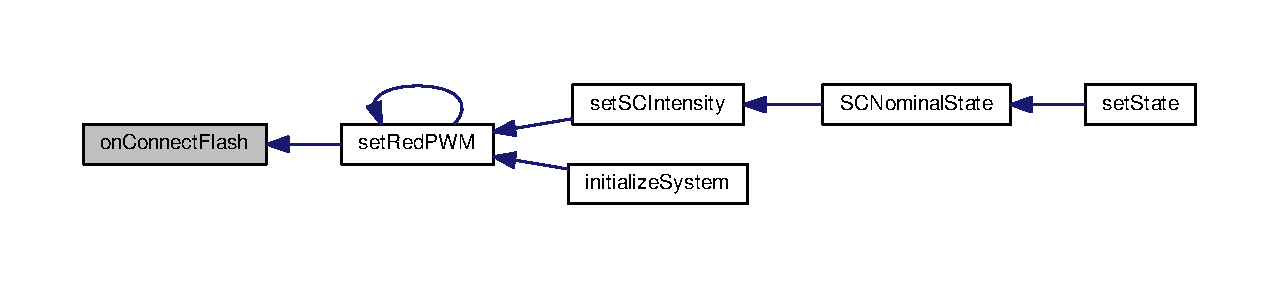
\includegraphics[width=350pt]{LEDControlManager_8h_ad3ec9b8ca1fb8ab67b960876b5761b42_icgraph}
\end{center}
\end{figure}


\index{L\+E\+D\+Control\+Manager.\+h@{L\+E\+D\+Control\+Manager.\+h}!on\+Disconnect\+Flash@{on\+Disconnect\+Flash}}
\index{on\+Disconnect\+Flash@{on\+Disconnect\+Flash}!L\+E\+D\+Control\+Manager.\+h@{L\+E\+D\+Control\+Manager.\+h}}
\subsubsection[{\texorpdfstring{on\+Disconnect\+Flash(void)}{onDisconnectFlash(void)}}]{\setlength{\rightskip}{0pt plus 5cm}void on\+Disconnect\+Flash (
\begin{DoxyParamCaption}
\item[{void}]{}
\end{DoxyParamCaption}
)}\hypertarget{LEDControlManager_8h_a9e6967c01a7e2bfae8a3281ef3eb02c4}{}\label{LEDControlManager_8h_a9e6967c01a7e2bfae8a3281ef3eb02c4}


Here is the caller graph for this function\+:
\nopagebreak
\begin{figure}[H]
\begin{center}
\leavevmode
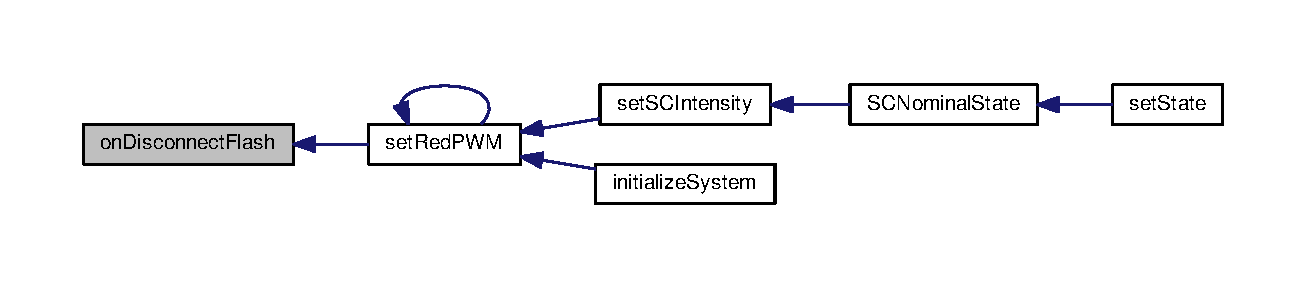
\includegraphics[width=350pt]{LEDControlManager_8h_a9e6967c01a7e2bfae8a3281ef3eb02c4_icgraph}
\end{center}
\end{figure}


\index{L\+E\+D\+Control\+Manager.\+h@{L\+E\+D\+Control\+Manager.\+h}!set\+Blue\+P\+WM@{set\+Blue\+P\+WM}}
\index{set\+Blue\+P\+WM@{set\+Blue\+P\+WM}!L\+E\+D\+Control\+Manager.\+h@{L\+E\+D\+Control\+Manager.\+h}}
\subsubsection[{\texorpdfstring{set\+Blue\+P\+W\+M(char percent)}{setBluePWM(char percent)}}]{\setlength{\rightskip}{0pt plus 5cm}void set\+Blue\+P\+WM (
\begin{DoxyParamCaption}
\item[{char}]{percent}
\end{DoxyParamCaption}
)}\hypertarget{LEDControlManager_8h_a91457a286ce7ad9931a802f91dd1542c}{}\label{LEDControlManager_8h_a91457a286ce7ad9931a802f91dd1542c}


Here is the caller graph for this function\+:
\nopagebreak
\begin{figure}[H]
\begin{center}
\leavevmode
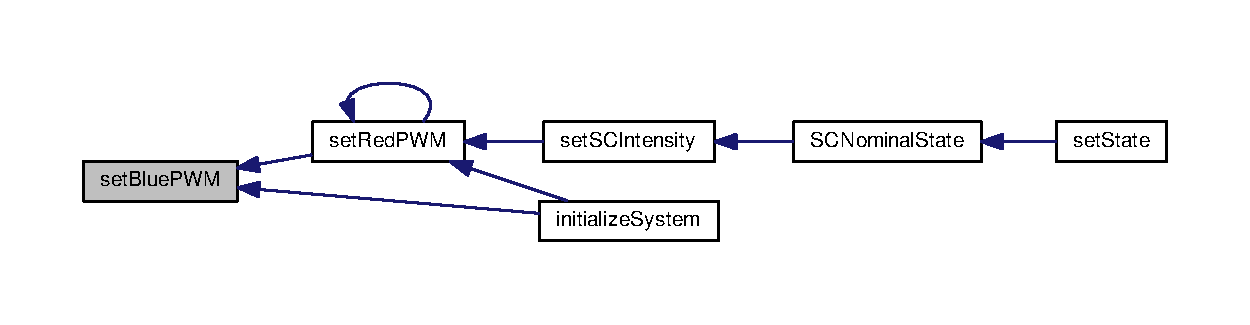
\includegraphics[width=350pt]{LEDControlManager_8h_a91457a286ce7ad9931a802f91dd1542c_icgraph}
\end{center}
\end{figure}


\index{L\+E\+D\+Control\+Manager.\+h@{L\+E\+D\+Control\+Manager.\+h}!set\+Green\+P\+WM@{set\+Green\+P\+WM}}
\index{set\+Green\+P\+WM@{set\+Green\+P\+WM}!L\+E\+D\+Control\+Manager.\+h@{L\+E\+D\+Control\+Manager.\+h}}
\subsubsection[{\texorpdfstring{set\+Green\+P\+W\+M(char percent)}{setGreenPWM(char percent)}}]{\setlength{\rightskip}{0pt plus 5cm}void set\+Green\+P\+WM (
\begin{DoxyParamCaption}
\item[{char}]{percent}
\end{DoxyParamCaption}
)}\hypertarget{LEDControlManager_8h_a5f7040b85d3431166dad2842730f077c}{}\label{LEDControlManager_8h_a5f7040b85d3431166dad2842730f077c}


Here is the caller graph for this function\+:
\nopagebreak
\begin{figure}[H]
\begin{center}
\leavevmode
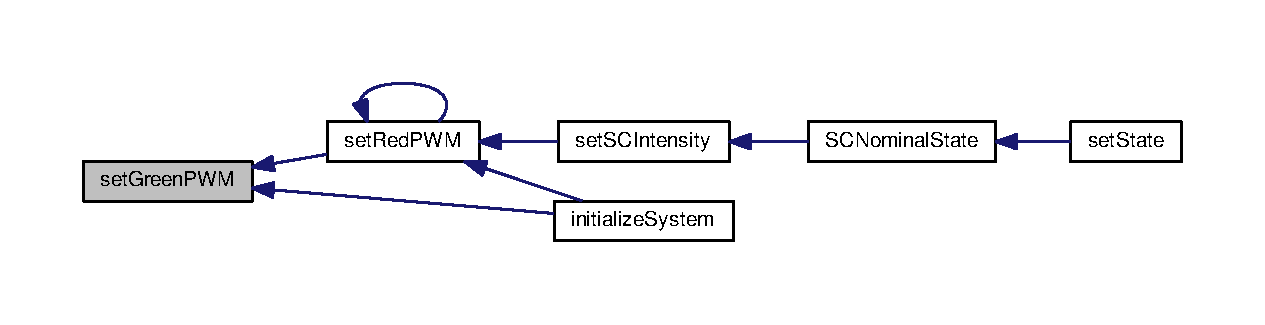
\includegraphics[width=350pt]{LEDControlManager_8h_a5f7040b85d3431166dad2842730f077c_icgraph}
\end{center}
\end{figure}


\index{L\+E\+D\+Control\+Manager.\+h@{L\+E\+D\+Control\+Manager.\+h}!set\+Red\+P\+WM@{set\+Red\+P\+WM}}
\index{set\+Red\+P\+WM@{set\+Red\+P\+WM}!L\+E\+D\+Control\+Manager.\+h@{L\+E\+D\+Control\+Manager.\+h}}
\subsubsection[{\texorpdfstring{set\+Red\+P\+W\+M(char percent)}{setRedPWM(char percent)}}]{\setlength{\rightskip}{0pt plus 5cm}void set\+Red\+P\+WM (
\begin{DoxyParamCaption}
\item[{char}]{percent}
\end{DoxyParamCaption}
)}\hypertarget{LEDControlManager_8h_a44568cbb326ce94b800b1407bd74c3a3}{}\label{LEDControlManager_8h_a44568cbb326ce94b800b1407bd74c3a3}


Here is the call graph for this function\+:
\nopagebreak
\begin{figure}[H]
\begin{center}
\leavevmode
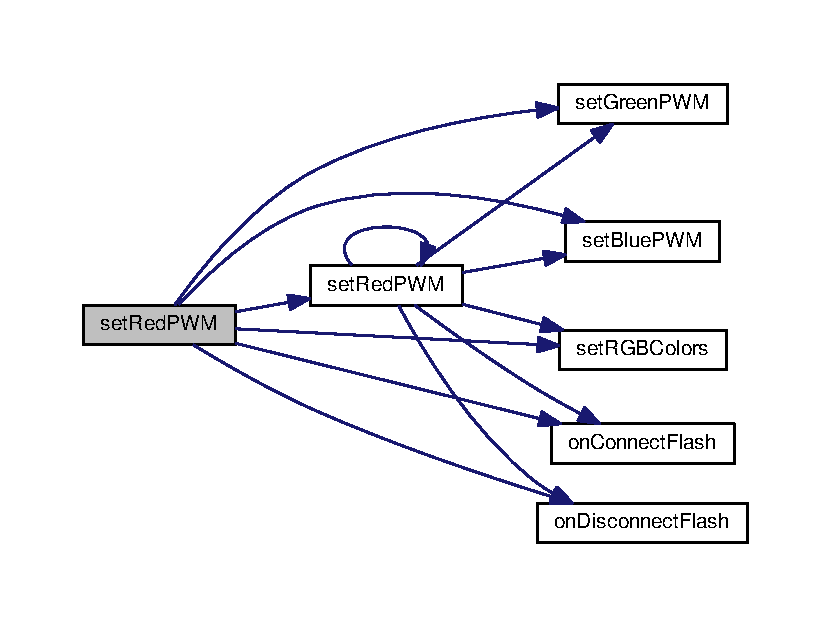
\includegraphics[width=350pt]{LEDControlManager_8h_a44568cbb326ce94b800b1407bd74c3a3_cgraph}
\end{center}
\end{figure}




Here is the caller graph for this function\+:
\nopagebreak
\begin{figure}[H]
\begin{center}
\leavevmode
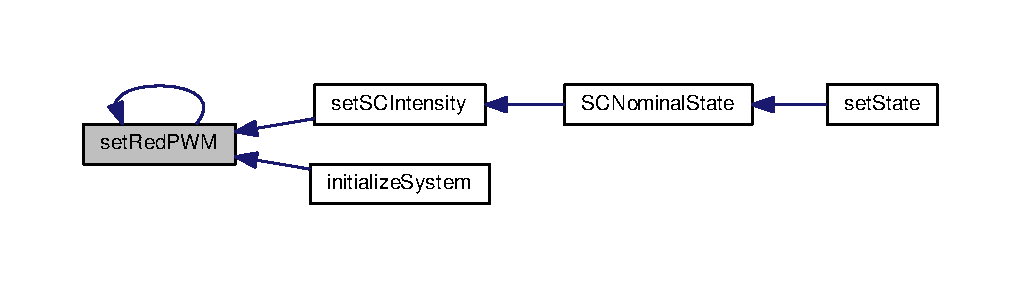
\includegraphics[width=350pt]{LEDControlManager_8h_a44568cbb326ce94b800b1407bd74c3a3_icgraph}
\end{center}
\end{figure}


\index{L\+E\+D\+Control\+Manager.\+h@{L\+E\+D\+Control\+Manager.\+h}!set\+R\+G\+B\+Colors@{set\+R\+G\+B\+Colors}}
\index{set\+R\+G\+B\+Colors@{set\+R\+G\+B\+Colors}!L\+E\+D\+Control\+Manager.\+h@{L\+E\+D\+Control\+Manager.\+h}}
\subsubsection[{\texorpdfstring{set\+R\+G\+B\+Colors(void)}{setRGBColors(void)}}]{\setlength{\rightskip}{0pt plus 5cm}void set\+R\+G\+B\+Colors (
\begin{DoxyParamCaption}
\item[{void}]{}
\end{DoxyParamCaption}
)}\hypertarget{LEDControlManager_8h_a63e99d1d357e27cdba2122126293ac7a}{}\label{LEDControlManager_8h_a63e99d1d357e27cdba2122126293ac7a}


Here is the caller graph for this function\+:
\nopagebreak
\begin{figure}[H]
\begin{center}
\leavevmode
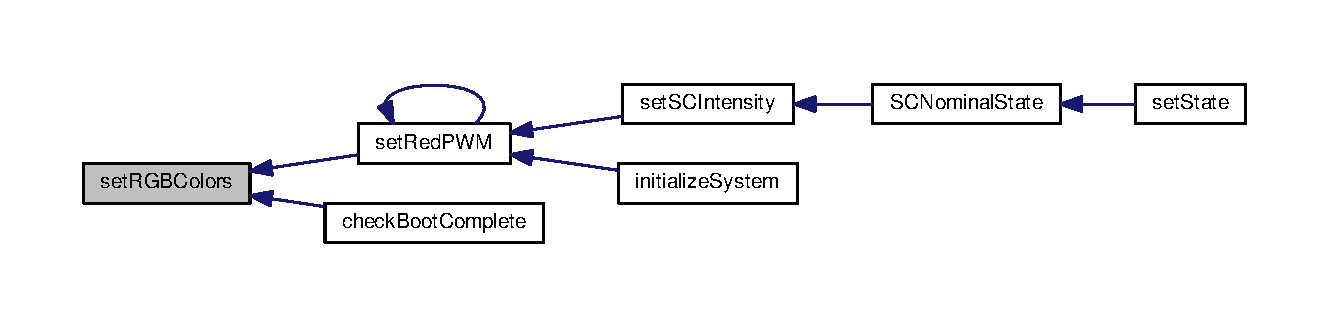
\includegraphics[width=350pt]{LEDControlManager_8h_a63e99d1d357e27cdba2122126293ac7a_icgraph}
\end{center}
\end{figure}


\index{L\+E\+D\+Control\+Manager.\+h@{L\+E\+D\+Control\+Manager.\+h}!set\+S\+C\+Intensity@{set\+S\+C\+Intensity}}
\index{set\+S\+C\+Intensity@{set\+S\+C\+Intensity}!L\+E\+D\+Control\+Manager.\+h@{L\+E\+D\+Control\+Manager.\+h}}
\subsubsection[{\texorpdfstring{set\+S\+C\+Intensity(void)}{setSCIntensity(void)}}]{\setlength{\rightskip}{0pt plus 5cm}void set\+S\+C\+Intensity (
\begin{DoxyParamCaption}
\item[{void}]{}
\end{DoxyParamCaption}
)}\hypertarget{LEDControlManager_8h_a1fb733347d7b1ebbae42b0078ede5453}{}\label{LEDControlManager_8h_a1fb733347d7b1ebbae42b0078ede5453}


Here is the call graph for this function\+:
\nopagebreak
\begin{figure}[H]
\begin{center}
\leavevmode
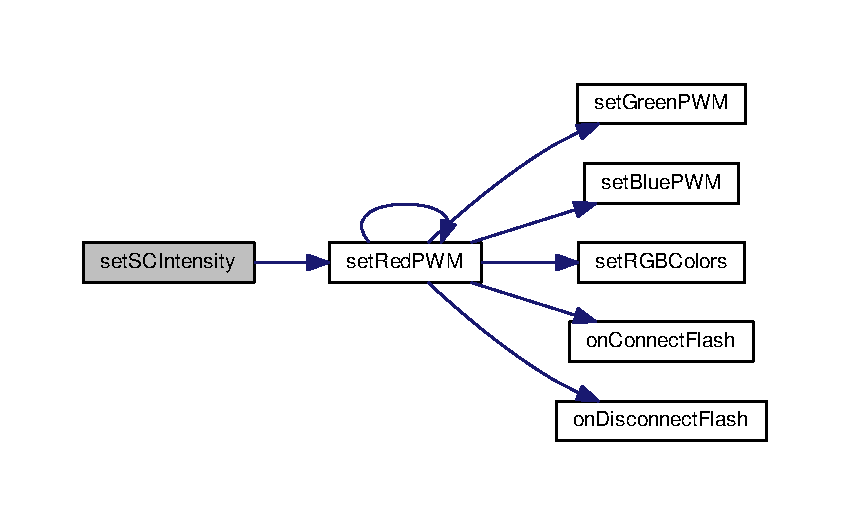
\includegraphics[width=350pt]{LEDControlManager_8h_a1fb733347d7b1ebbae42b0078ede5453_cgraph}
\end{center}
\end{figure}




Here is the caller graph for this function\+:
\nopagebreak
\begin{figure}[H]
\begin{center}
\leavevmode
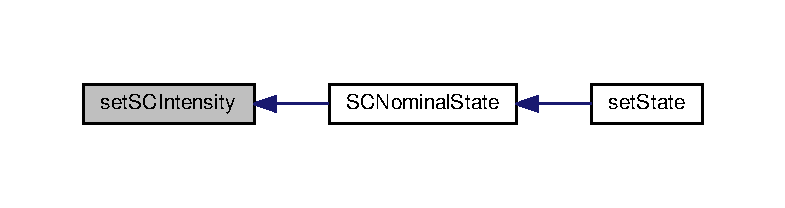
\includegraphics[width=350pt]{LEDControlManager_8h_a1fb733347d7b1ebbae42b0078ede5453_icgraph}
\end{center}
\end{figure}



\hypertarget{Memory_8c}{}\section{Memory.\+c File Reference}
\label{Memory_8c}\index{Memory.\+c@{Memory.\+c}}

\hypertarget{Memory_8h}{}\section{Memory.\+h File Reference}
\label{Memory_8h}\index{Memory.\+h@{Memory.\+h}}
{\ttfamily \#include $<$Arduino.\+h$>$}\\*
Include dependency graph for Memory.\+h\+:
\nopagebreak
\begin{figure}[H]
\begin{center}
\leavevmode
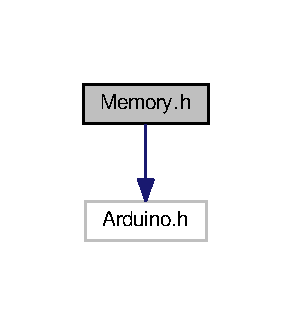
\includegraphics[width=140pt]{Memory_8h__incl}
\end{center}
\end{figure}
\subsection*{Macros}
\begin{DoxyCompactItemize}
\item 
\#define \hyperlink{Memory_8h_aa03d1cf73552f8a73187149911a1e666}{M\+A\+X\+\_\+\+N\+U\+M\+B\+E\+R\+\_\+\+O\+F\+\_\+\+F\+L\+A\+S\+H\+\_\+\+W\+R\+I\+T\+ES}~18000
\item 
\#define \hyperlink{Memory_8h_a0ef21bc8ac11011fca0de0ed8d27e2a3}{T\+I\+M\+E\+\_\+\+O\+F\+\_\+\+U\+S\+E\+\_\+\+P\+E\+R\+I\+O\+D\+\_\+\+I\+N\+\_\+\+MS}~600000
\end{DoxyCompactItemize}


\subsection{Macro Definition Documentation}
\index{Memory.\+h@{Memory.\+h}!M\+A\+X\+\_\+\+N\+U\+M\+B\+E\+R\+\_\+\+O\+F\+\_\+\+F\+L\+A\+S\+H\+\_\+\+W\+R\+I\+T\+ES@{M\+A\+X\+\_\+\+N\+U\+M\+B\+E\+R\+\_\+\+O\+F\+\_\+\+F\+L\+A\+S\+H\+\_\+\+W\+R\+I\+T\+ES}}
\index{M\+A\+X\+\_\+\+N\+U\+M\+B\+E\+R\+\_\+\+O\+F\+\_\+\+F\+L\+A\+S\+H\+\_\+\+W\+R\+I\+T\+ES@{M\+A\+X\+\_\+\+N\+U\+M\+B\+E\+R\+\_\+\+O\+F\+\_\+\+F\+L\+A\+S\+H\+\_\+\+W\+R\+I\+T\+ES}!Memory.\+h@{Memory.\+h}}
\subsubsection[{\texorpdfstring{M\+A\+X\+\_\+\+N\+U\+M\+B\+E\+R\+\_\+\+O\+F\+\_\+\+F\+L\+A\+S\+H\+\_\+\+W\+R\+I\+T\+ES}{MAX_NUMBER_OF_FLASH_WRITES}}]{\setlength{\rightskip}{0pt plus 5cm}\#define M\+A\+X\+\_\+\+N\+U\+M\+B\+E\+R\+\_\+\+O\+F\+\_\+\+F\+L\+A\+S\+H\+\_\+\+W\+R\+I\+T\+ES~18000}\hypertarget{Memory_8h_aa03d1cf73552f8a73187149911a1e666}{}\label{Memory_8h_aa03d1cf73552f8a73187149911a1e666}
\index{Memory.\+h@{Memory.\+h}!T\+I\+M\+E\+\_\+\+O\+F\+\_\+\+U\+S\+E\+\_\+\+P\+E\+R\+I\+O\+D\+\_\+\+I\+N\+\_\+\+MS@{T\+I\+M\+E\+\_\+\+O\+F\+\_\+\+U\+S\+E\+\_\+\+P\+E\+R\+I\+O\+D\+\_\+\+I\+N\+\_\+\+MS}}
\index{T\+I\+M\+E\+\_\+\+O\+F\+\_\+\+U\+S\+E\+\_\+\+P\+E\+R\+I\+O\+D\+\_\+\+I\+N\+\_\+\+MS@{T\+I\+M\+E\+\_\+\+O\+F\+\_\+\+U\+S\+E\+\_\+\+P\+E\+R\+I\+O\+D\+\_\+\+I\+N\+\_\+\+MS}!Memory.\+h@{Memory.\+h}}
\subsubsection[{\texorpdfstring{T\+I\+M\+E\+\_\+\+O\+F\+\_\+\+U\+S\+E\+\_\+\+P\+E\+R\+I\+O\+D\+\_\+\+I\+N\+\_\+\+MS}{TIME_OF_USE_PERIOD_IN_MS}}]{\setlength{\rightskip}{0pt plus 5cm}\#define T\+I\+M\+E\+\_\+\+O\+F\+\_\+\+U\+S\+E\+\_\+\+P\+E\+R\+I\+O\+D\+\_\+\+I\+N\+\_\+\+MS~600000}\hypertarget{Memory_8h_a0ef21bc8ac11011fca0de0ed8d27e2a3}{}\label{Memory_8h_a0ef21bc8ac11011fca0de0ed8d27e2a3}

\hypertarget{PinDefinitions_8h}{}\section{Pin\+Definitions.\+h File Reference}
\label{PinDefinitions_8h}\index{Pin\+Definitions.\+h@{Pin\+Definitions.\+h}}
This graph shows which files directly or indirectly include this file\+:
\nopagebreak
\begin{figure}[H]
\begin{center}
\leavevmode
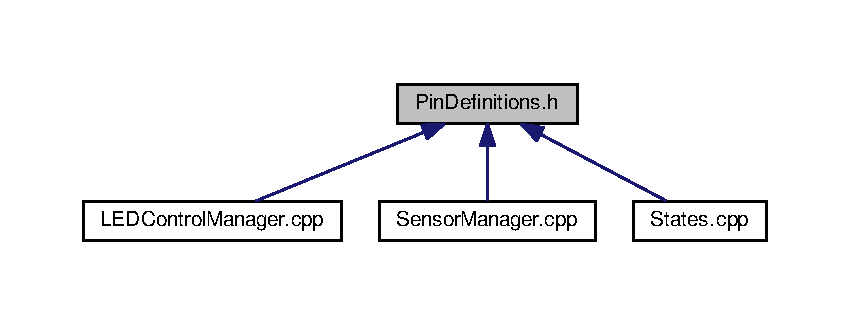
\includegraphics[width=350pt]{PinDefinitions_8h__dep__incl}
\end{center}
\end{figure}
\subsection*{Macros}
\begin{DoxyCompactItemize}
\item 
\#define \hyperlink{PinDefinitions_8h_ab16f55d54417647f44dca8b11d988f02}{R\+E\+D\+\_\+\+L\+E\+D\+\_\+\+P\+IN}~4
\item 
\#define \hyperlink{PinDefinitions_8h_a8131714b6d25634105b1122f222dca26}{G\+R\+E\+E\+N\+\_\+\+L\+E\+D\+\_\+\+P\+IN}~5
\item 
\#define \hyperlink{PinDefinitions_8h_a5a8a44baec34d5355cbfdb6d16786f84}{B\+L\+U\+E\+\_\+\+L\+E\+D\+\_\+\+P\+IN}~6
\item 
\#define \hyperlink{PinDefinitions_8h_aa27202491fadec5fa1975d0a5ca07ca6}{L\+E\+D\+\_\+\+B\+O\+A\+R\+D\+\_\+\+T\+E\+M\+P\+\_\+\+P\+IN}~2
\item 
\#define \hyperlink{PinDefinitions_8h_a37d5da9e960f09876caaa0d5bbdb4c6a}{I\+N\+P\+U\+T\+\_\+\+V\+O\+L\+T\+A\+G\+E\+\_\+\+P\+IN}~1
\end{DoxyCompactItemize}


\subsection{Macro Definition Documentation}
\index{Pin\+Definitions.\+h@{Pin\+Definitions.\+h}!B\+L\+U\+E\+\_\+\+L\+E\+D\+\_\+\+P\+IN@{B\+L\+U\+E\+\_\+\+L\+E\+D\+\_\+\+P\+IN}}
\index{B\+L\+U\+E\+\_\+\+L\+E\+D\+\_\+\+P\+IN@{B\+L\+U\+E\+\_\+\+L\+E\+D\+\_\+\+P\+IN}!Pin\+Definitions.\+h@{Pin\+Definitions.\+h}}
\subsubsection[{\texorpdfstring{B\+L\+U\+E\+\_\+\+L\+E\+D\+\_\+\+P\+IN}{BLUE_LED_PIN}}]{\setlength{\rightskip}{0pt plus 5cm}\#define B\+L\+U\+E\+\_\+\+L\+E\+D\+\_\+\+P\+IN~6}\hypertarget{PinDefinitions_8h_a5a8a44baec34d5355cbfdb6d16786f84}{}\label{PinDefinitions_8h_a5a8a44baec34d5355cbfdb6d16786f84}
\index{Pin\+Definitions.\+h@{Pin\+Definitions.\+h}!G\+R\+E\+E\+N\+\_\+\+L\+E\+D\+\_\+\+P\+IN@{G\+R\+E\+E\+N\+\_\+\+L\+E\+D\+\_\+\+P\+IN}}
\index{G\+R\+E\+E\+N\+\_\+\+L\+E\+D\+\_\+\+P\+IN@{G\+R\+E\+E\+N\+\_\+\+L\+E\+D\+\_\+\+P\+IN}!Pin\+Definitions.\+h@{Pin\+Definitions.\+h}}
\subsubsection[{\texorpdfstring{G\+R\+E\+E\+N\+\_\+\+L\+E\+D\+\_\+\+P\+IN}{GREEN_LED_PIN}}]{\setlength{\rightskip}{0pt plus 5cm}\#define G\+R\+E\+E\+N\+\_\+\+L\+E\+D\+\_\+\+P\+IN~5}\hypertarget{PinDefinitions_8h_a8131714b6d25634105b1122f222dca26}{}\label{PinDefinitions_8h_a8131714b6d25634105b1122f222dca26}
\index{Pin\+Definitions.\+h@{Pin\+Definitions.\+h}!I\+N\+P\+U\+T\+\_\+\+V\+O\+L\+T\+A\+G\+E\+\_\+\+P\+IN@{I\+N\+P\+U\+T\+\_\+\+V\+O\+L\+T\+A\+G\+E\+\_\+\+P\+IN}}
\index{I\+N\+P\+U\+T\+\_\+\+V\+O\+L\+T\+A\+G\+E\+\_\+\+P\+IN@{I\+N\+P\+U\+T\+\_\+\+V\+O\+L\+T\+A\+G\+E\+\_\+\+P\+IN}!Pin\+Definitions.\+h@{Pin\+Definitions.\+h}}
\subsubsection[{\texorpdfstring{I\+N\+P\+U\+T\+\_\+\+V\+O\+L\+T\+A\+G\+E\+\_\+\+P\+IN}{INPUT_VOLTAGE_PIN}}]{\setlength{\rightskip}{0pt plus 5cm}\#define I\+N\+P\+U\+T\+\_\+\+V\+O\+L\+T\+A\+G\+E\+\_\+\+P\+IN~1}\hypertarget{PinDefinitions_8h_a37d5da9e960f09876caaa0d5bbdb4c6a}{}\label{PinDefinitions_8h_a37d5da9e960f09876caaa0d5bbdb4c6a}
\index{Pin\+Definitions.\+h@{Pin\+Definitions.\+h}!L\+E\+D\+\_\+\+B\+O\+A\+R\+D\+\_\+\+T\+E\+M\+P\+\_\+\+P\+IN@{L\+E\+D\+\_\+\+B\+O\+A\+R\+D\+\_\+\+T\+E\+M\+P\+\_\+\+P\+IN}}
\index{L\+E\+D\+\_\+\+B\+O\+A\+R\+D\+\_\+\+T\+E\+M\+P\+\_\+\+P\+IN@{L\+E\+D\+\_\+\+B\+O\+A\+R\+D\+\_\+\+T\+E\+M\+P\+\_\+\+P\+IN}!Pin\+Definitions.\+h@{Pin\+Definitions.\+h}}
\subsubsection[{\texorpdfstring{L\+E\+D\+\_\+\+B\+O\+A\+R\+D\+\_\+\+T\+E\+M\+P\+\_\+\+P\+IN}{LED_BOARD_TEMP_PIN}}]{\setlength{\rightskip}{0pt plus 5cm}\#define L\+E\+D\+\_\+\+B\+O\+A\+R\+D\+\_\+\+T\+E\+M\+P\+\_\+\+P\+IN~2}\hypertarget{PinDefinitions_8h_aa27202491fadec5fa1975d0a5ca07ca6}{}\label{PinDefinitions_8h_aa27202491fadec5fa1975d0a5ca07ca6}
\index{Pin\+Definitions.\+h@{Pin\+Definitions.\+h}!R\+E\+D\+\_\+\+L\+E\+D\+\_\+\+P\+IN@{R\+E\+D\+\_\+\+L\+E\+D\+\_\+\+P\+IN}}
\index{R\+E\+D\+\_\+\+L\+E\+D\+\_\+\+P\+IN@{R\+E\+D\+\_\+\+L\+E\+D\+\_\+\+P\+IN}!Pin\+Definitions.\+h@{Pin\+Definitions.\+h}}
\subsubsection[{\texorpdfstring{R\+E\+D\+\_\+\+L\+E\+D\+\_\+\+P\+IN}{RED_LED_PIN}}]{\setlength{\rightskip}{0pt plus 5cm}\#define R\+E\+D\+\_\+\+L\+E\+D\+\_\+\+P\+IN~4}\hypertarget{PinDefinitions_8h_ab16f55d54417647f44dca8b11d988f02}{}\label{PinDefinitions_8h_ab16f55d54417647f44dca8b11d988f02}

\hypertarget{SensorManager_8cpp}{}\section{Sensor\+Manager.\+cpp File Reference}
\label{SensorManager_8cpp}\index{Sensor\+Manager.\+cpp@{Sensor\+Manager.\+cpp}}
{\ttfamily \#include \char`\"{}Sensor\+Manager.\+h\char`\"{}}\\*
{\ttfamily \#include $<$Arduino.\+h$>$}\\*
{\ttfamily \#include \char`\"{}Globals.\+h\char`\"{}}\\*
{\ttfamily \#include \char`\"{}Pin\+Definitions.\+h\char`\"{}}\\*
{\ttfamily \#include \char`\"{}Serial\+Debug.\+h\char`\"{}}\\*
Include dependency graph for Sensor\+Manager.\+cpp\+:
\nopagebreak
\begin{figure}[H]
\begin{center}
\leavevmode
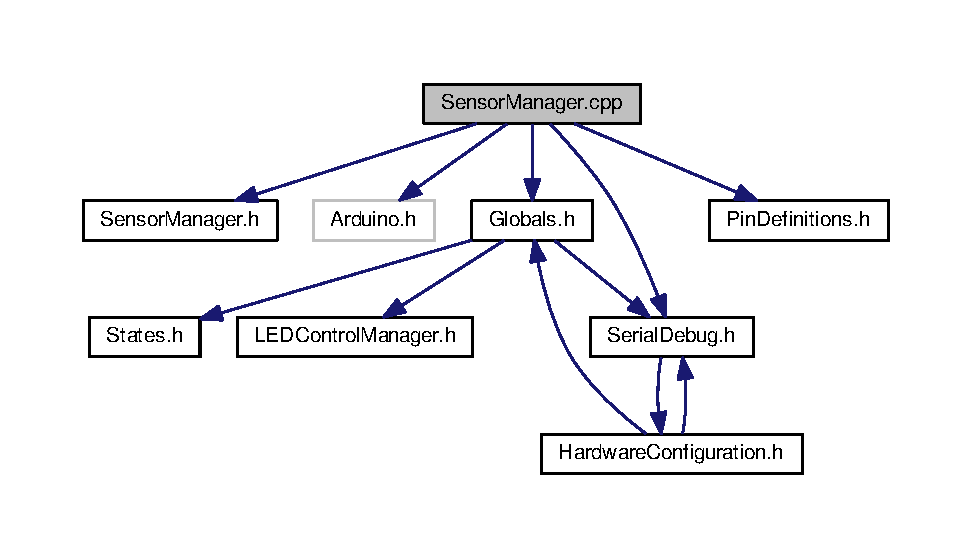
\includegraphics[width=350pt]{SensorManager_8cpp__incl}
\end{center}
\end{figure}
\subsection*{Functions}
\begin{DoxyCompactItemize}
\item 
int \hyperlink{SensorManager_8cpp_a1c943d491d2f32971f84a2eecdf00f2e}{get\+L\+E\+D\+TempinC} (void)
\item 
float \hyperlink{SensorManager_8cpp_a2bc89f165614192d9972b8259a6a45e7}{get\+Input\+VoltageinV} (void)
\item 
void \hyperlink{SensorManager_8cpp_ab791afb3dfb01137d61ffcc1a312ade5}{check\+Sensors} (void)
\end{DoxyCompactItemize}
\subsection*{Variables}
\begin{DoxyCompactItemize}
\item 
class \hyperlink{classTimerClass}{Timer\+Class} \hyperlink{SensorManager_8cpp_aad730ad0eae96403c695f303b895c869}{Voltage\+Time}
\item 
struct \hyperlink{structsensorFeedback}{sensor\+Feedback} \hyperlink{SensorManager_8cpp_ac36c738a70d60c7bcc58fa8bc43d50d7}{sensor\+Feedback}
\end{DoxyCompactItemize}


\subsection{Function Documentation}
\index{Sensor\+Manager.\+cpp@{Sensor\+Manager.\+cpp}!check\+Sensors@{check\+Sensors}}
\index{check\+Sensors@{check\+Sensors}!Sensor\+Manager.\+cpp@{Sensor\+Manager.\+cpp}}
\subsubsection[{\texorpdfstring{check\+Sensors(void)}{checkSensors(void)}}]{\setlength{\rightskip}{0pt plus 5cm}void check\+Sensors (
\begin{DoxyParamCaption}
\item[{void}]{}
\end{DoxyParamCaption}
)}\hypertarget{SensorManager_8cpp_ab791afb3dfb01137d61ffcc1a312ade5}{}\label{SensorManager_8cpp_ab791afb3dfb01137d61ffcc1a312ade5}


Here is the call graph for this function\+:
\nopagebreak
\begin{figure}[H]
\begin{center}
\leavevmode
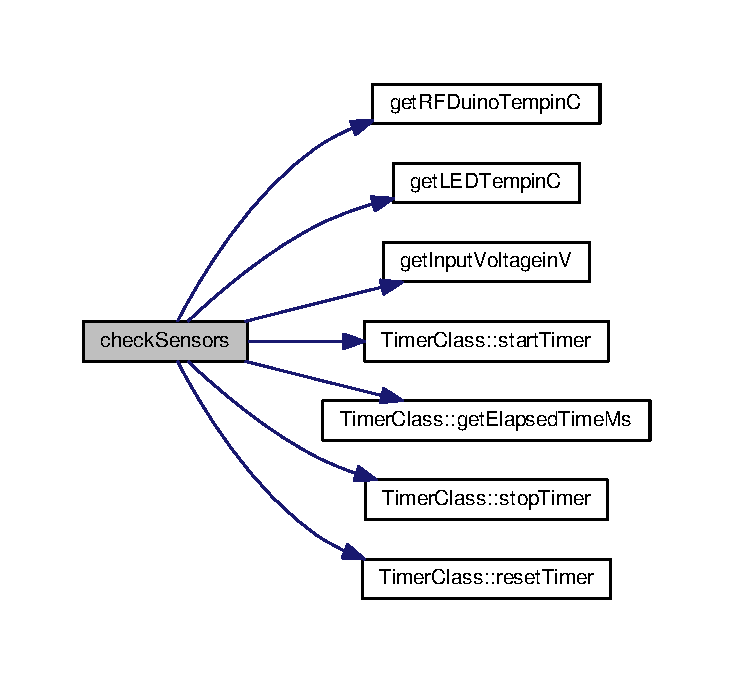
\includegraphics[width=350pt]{SensorManager_8cpp_ab791afb3dfb01137d61ffcc1a312ade5_cgraph}
\end{center}
\end{figure}




Here is the caller graph for this function\+:
\nopagebreak
\begin{figure}[H]
\begin{center}
\leavevmode
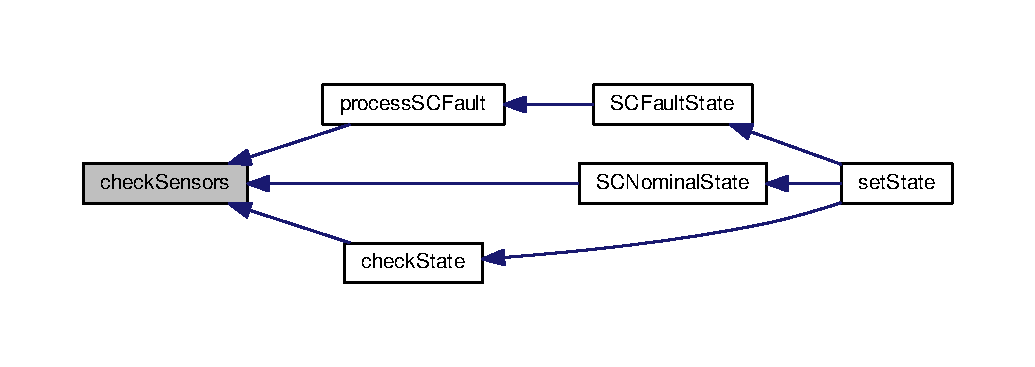
\includegraphics[width=350pt]{SensorManager_8cpp_ab791afb3dfb01137d61ffcc1a312ade5_icgraph}
\end{center}
\end{figure}


\index{Sensor\+Manager.\+cpp@{Sensor\+Manager.\+cpp}!get\+Input\+VoltageinV@{get\+Input\+VoltageinV}}
\index{get\+Input\+VoltageinV@{get\+Input\+VoltageinV}!Sensor\+Manager.\+cpp@{Sensor\+Manager.\+cpp}}
\subsubsection[{\texorpdfstring{get\+Input\+Voltagein\+V(void)}{getInputVoltageinV(void)}}]{\setlength{\rightskip}{0pt plus 5cm}float get\+Input\+VoltageinV (
\begin{DoxyParamCaption}
\item[{void}]{}
\end{DoxyParamCaption}
)}\hypertarget{SensorManager_8cpp_a2bc89f165614192d9972b8259a6a45e7}{}\label{SensorManager_8cpp_a2bc89f165614192d9972b8259a6a45e7}


Here is the caller graph for this function\+:
\nopagebreak
\begin{figure}[H]
\begin{center}
\leavevmode
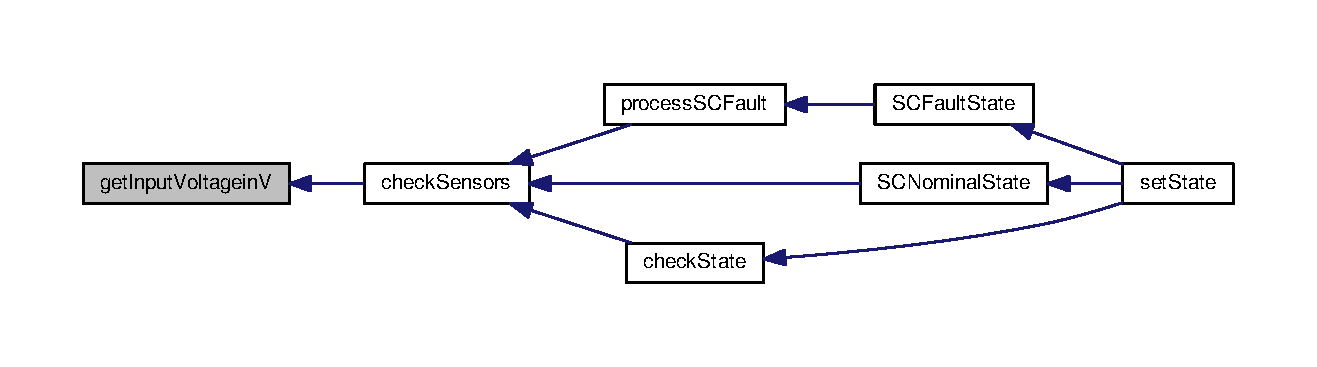
\includegraphics[width=350pt]{SensorManager_8cpp_a2bc89f165614192d9972b8259a6a45e7_icgraph}
\end{center}
\end{figure}


\index{Sensor\+Manager.\+cpp@{Sensor\+Manager.\+cpp}!get\+L\+E\+D\+TempinC@{get\+L\+E\+D\+TempinC}}
\index{get\+L\+E\+D\+TempinC@{get\+L\+E\+D\+TempinC}!Sensor\+Manager.\+cpp@{Sensor\+Manager.\+cpp}}
\subsubsection[{\texorpdfstring{get\+L\+E\+D\+Tempin\+C(void)}{getLEDTempinC(void)}}]{\setlength{\rightskip}{0pt plus 5cm}int get\+L\+E\+D\+TempinC (
\begin{DoxyParamCaption}
\item[{void}]{}
\end{DoxyParamCaption}
)}\hypertarget{SensorManager_8cpp_a1c943d491d2f32971f84a2eecdf00f2e}{}\label{SensorManager_8cpp_a1c943d491d2f32971f84a2eecdf00f2e}


Here is the caller graph for this function\+:
\nopagebreak
\begin{figure}[H]
\begin{center}
\leavevmode
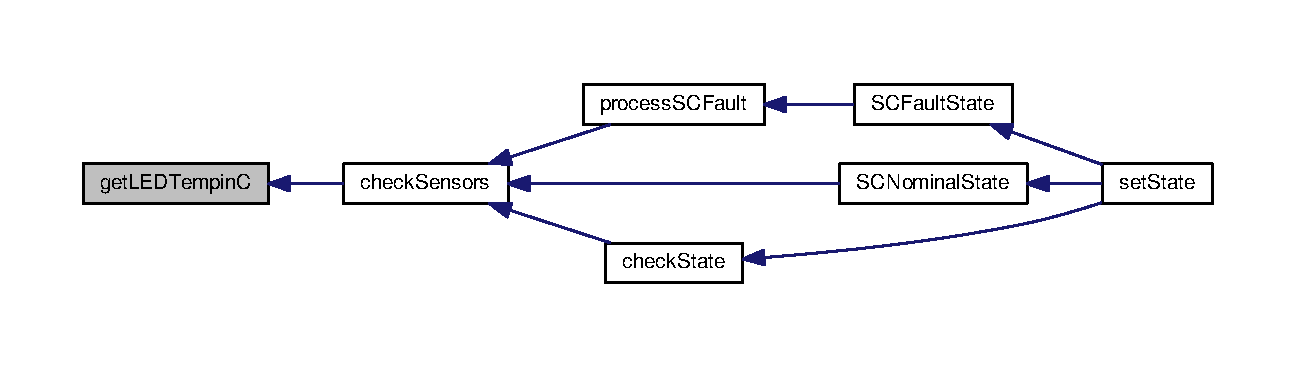
\includegraphics[width=350pt]{SensorManager_8cpp_a1c943d491d2f32971f84a2eecdf00f2e_icgraph}
\end{center}
\end{figure}




\subsection{Variable Documentation}
\index{Sensor\+Manager.\+cpp@{Sensor\+Manager.\+cpp}!sensor\+Feedback@{sensor\+Feedback}}
\index{sensor\+Feedback@{sensor\+Feedback}!Sensor\+Manager.\+cpp@{Sensor\+Manager.\+cpp}}
\subsubsection[{\texorpdfstring{sensor\+Feedback}{sensorFeedback}}]{\setlength{\rightskip}{0pt plus 5cm}struct {\bf sensor\+Feedback} {\bf sensor\+Feedback}}\hypertarget{SensorManager_8cpp_ac36c738a70d60c7bcc58fa8bc43d50d7}{}\label{SensorManager_8cpp_ac36c738a70d60c7bcc58fa8bc43d50d7}
\index{Sensor\+Manager.\+cpp@{Sensor\+Manager.\+cpp}!Voltage\+Time@{Voltage\+Time}}
\index{Voltage\+Time@{Voltage\+Time}!Sensor\+Manager.\+cpp@{Sensor\+Manager.\+cpp}}
\subsubsection[{\texorpdfstring{Voltage\+Time}{VoltageTime}}]{\setlength{\rightskip}{0pt plus 5cm}class {\bf Timer\+Class} Voltage\+Time}\hypertarget{SensorManager_8cpp_aad730ad0eae96403c695f303b895c869}{}\label{SensorManager_8cpp_aad730ad0eae96403c695f303b895c869}

\hypertarget{SensorManager_8h}{}\section{Sensor\+Manager.\+h File Reference}
\label{SensorManager_8h}\index{Sensor\+Manager.\+h@{Sensor\+Manager.\+h}}
This graph shows which files directly or indirectly include this file\+:
\nopagebreak
\begin{figure}[H]
\begin{center}
\leavevmode
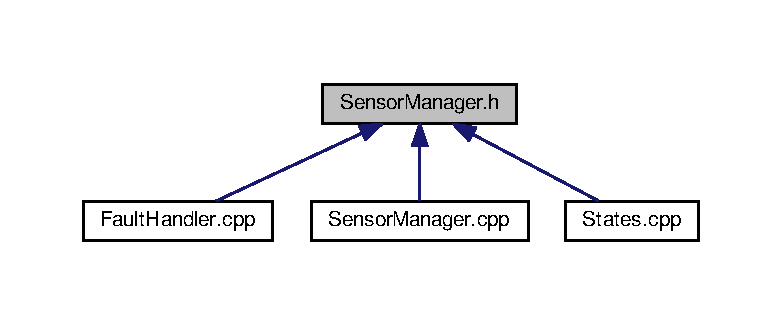
\includegraphics[width=350pt]{SensorManager_8h__dep__incl}
\end{center}
\end{figure}
\subsection*{Classes}
\begin{DoxyCompactItemize}
\item 
struct \hyperlink{structsensorFeedback}{sensor\+Feedback}
\begin{DoxyCompactList}\small\item\em \hyperlink{structsensorFeedback}{sensor\+Feedback} struct Description \end{DoxyCompactList}\end{DoxyCompactItemize}
\subsection*{Macros}
\begin{DoxyCompactItemize}
\item 
\#define \hyperlink{SensorManager_8h_a00978ca9e8220475258dcbbbb7d29129}{A\+D\+C\+\_\+\+R\+E\+S\+O\+L\+U\+T\+I\+ON}~1024
\item 
\#define \hyperlink{SensorManager_8h_a62862d7518b2e40d051ee8dd74f6661c}{A\+D\+C\+\_\+\+V\+O\+L\+T\+A\+G\+E\+\_\+\+R\+EF}~3.\+3
\item 
\#define \hyperlink{SensorManager_8h_aff9d7f22ffcae9a0dd4dfc76c28bf338}{R\+F\+D\+U\+I\+N\+O\+\_\+\+C\+R\+I\+T\+I\+C\+A\+L\+\_\+\+T\+E\+M\+P\+\_\+C}~60
\item 
\#define \hyperlink{SensorManager_8h_a4da1c001c2e03286aba861c1621817cf}{L\+E\+D\+\_\+\+W\+A\+R\+N\+I\+N\+G\+\_\+\+T\+E\+M\+P\+\_\+C}~60
\item 
\#define \hyperlink{SensorManager_8h_ab704702e8fd74ddc5d5f7a4224678c42}{L\+E\+D\+\_\+\+C\+R\+I\+T\+I\+C\+A\+L\+\_\+\+T\+E\+M\+P\+\_\+C}~70
\item 
\#define \hyperlink{SensorManager_8h_ab46703b3e35703940af407b62d7acb62}{I\+N\+P\+U\+T\+\_\+\+V\+O\+L\+T\+A\+G\+E\+\_\+\+W\+A\+R\+N\+I\+N\+G\+\_\+V}~12.\+7
\item 
\#define \hyperlink{SensorManager_8h_acbb5d7b19fb5b92d660d4681f9bc9238}{I\+N\+P\+U\+T\+\_\+\+V\+O\+L\+T\+A\+G\+E\+\_\+\+C\+R\+I\+T\+I\+C\+A\+L\+\_\+V}~12.\+1
\item 
\#define \hyperlink{SensorManager_8h_a0ebf6f6ffe11817da07d5c6168eaf6c5}{I\+N\+P\+U\+T\+\_\+\+V\+O\+L\+T\+A\+G\+E\+\_\+\+S\+A\+G\+\_\+\+T\+I\+M\+E\+\_\+\+MS}~7000
\end{DoxyCompactItemize}
\subsection*{Functions}
\begin{DoxyCompactItemize}
\item 
int \hyperlink{SensorManager_8h_a1b9f0e0ff57635f1e86c2c7fcddab439}{get\+R\+F\+Duino\+TempinC} (void)
\item 
int \hyperlink{SensorManager_8h_a1c943d491d2f32971f84a2eecdf00f2e}{get\+L\+E\+D\+TempinC} (void)
\item 
int \hyperlink{SensorManager_8h_aef3b6a94bf072b577b14b6bcdc1d6334}{get\+Input\+VoltageinmV} (void)
\item 
void \hyperlink{SensorManager_8h_ab791afb3dfb01137d61ffcc1a312ade5}{check\+Sensors} (void)
\end{DoxyCompactItemize}
\subsection*{Variables}
\begin{DoxyCompactItemize}
\item 
\hyperlink{structsensorFeedback}{sensor\+Feedback} \hyperlink{SensorManager_8h_a28902247617a380eadc4313c5df4c270}{sensor\+Feedback}
\end{DoxyCompactItemize}


\subsection{Macro Definition Documentation}
\index{Sensor\+Manager.\+h@{Sensor\+Manager.\+h}!A\+D\+C\+\_\+\+R\+E\+S\+O\+L\+U\+T\+I\+ON@{A\+D\+C\+\_\+\+R\+E\+S\+O\+L\+U\+T\+I\+ON}}
\index{A\+D\+C\+\_\+\+R\+E\+S\+O\+L\+U\+T\+I\+ON@{A\+D\+C\+\_\+\+R\+E\+S\+O\+L\+U\+T\+I\+ON}!Sensor\+Manager.\+h@{Sensor\+Manager.\+h}}
\subsubsection[{\texorpdfstring{A\+D\+C\+\_\+\+R\+E\+S\+O\+L\+U\+T\+I\+ON}{ADC_RESOLUTION}}]{\setlength{\rightskip}{0pt plus 5cm}\#define A\+D\+C\+\_\+\+R\+E\+S\+O\+L\+U\+T\+I\+ON~1024}\hypertarget{SensorManager_8h_a00978ca9e8220475258dcbbbb7d29129}{}\label{SensorManager_8h_a00978ca9e8220475258dcbbbb7d29129}
\index{Sensor\+Manager.\+h@{Sensor\+Manager.\+h}!A\+D\+C\+\_\+\+V\+O\+L\+T\+A\+G\+E\+\_\+\+R\+EF@{A\+D\+C\+\_\+\+V\+O\+L\+T\+A\+G\+E\+\_\+\+R\+EF}}
\index{A\+D\+C\+\_\+\+V\+O\+L\+T\+A\+G\+E\+\_\+\+R\+EF@{A\+D\+C\+\_\+\+V\+O\+L\+T\+A\+G\+E\+\_\+\+R\+EF}!Sensor\+Manager.\+h@{Sensor\+Manager.\+h}}
\subsubsection[{\texorpdfstring{A\+D\+C\+\_\+\+V\+O\+L\+T\+A\+G\+E\+\_\+\+R\+EF}{ADC_VOLTAGE_REF}}]{\setlength{\rightskip}{0pt plus 5cm}\#define A\+D\+C\+\_\+\+V\+O\+L\+T\+A\+G\+E\+\_\+\+R\+EF~3.\+3}\hypertarget{SensorManager_8h_a62862d7518b2e40d051ee8dd74f6661c}{}\label{SensorManager_8h_a62862d7518b2e40d051ee8dd74f6661c}
\index{Sensor\+Manager.\+h@{Sensor\+Manager.\+h}!I\+N\+P\+U\+T\+\_\+\+V\+O\+L\+T\+A\+G\+E\+\_\+\+C\+R\+I\+T\+I\+C\+A\+L\+\_\+V@{I\+N\+P\+U\+T\+\_\+\+V\+O\+L\+T\+A\+G\+E\+\_\+\+C\+R\+I\+T\+I\+C\+A\+L\+\_\+V}}
\index{I\+N\+P\+U\+T\+\_\+\+V\+O\+L\+T\+A\+G\+E\+\_\+\+C\+R\+I\+T\+I\+C\+A\+L\+\_\+V@{I\+N\+P\+U\+T\+\_\+\+V\+O\+L\+T\+A\+G\+E\+\_\+\+C\+R\+I\+T\+I\+C\+A\+L\+\_\+V}!Sensor\+Manager.\+h@{Sensor\+Manager.\+h}}
\subsubsection[{\texorpdfstring{I\+N\+P\+U\+T\+\_\+\+V\+O\+L\+T\+A\+G\+E\+\_\+\+C\+R\+I\+T\+I\+C\+A\+L\+\_\+V}{INPUT_VOLTAGE_CRITICAL_V}}]{\setlength{\rightskip}{0pt plus 5cm}\#define I\+N\+P\+U\+T\+\_\+\+V\+O\+L\+T\+A\+G\+E\+\_\+\+C\+R\+I\+T\+I\+C\+A\+L\+\_\+V~12.\+1}\hypertarget{SensorManager_8h_acbb5d7b19fb5b92d660d4681f9bc9238}{}\label{SensorManager_8h_acbb5d7b19fb5b92d660d4681f9bc9238}
\index{Sensor\+Manager.\+h@{Sensor\+Manager.\+h}!I\+N\+P\+U\+T\+\_\+\+V\+O\+L\+T\+A\+G\+E\+\_\+\+S\+A\+G\+\_\+\+T\+I\+M\+E\+\_\+\+MS@{I\+N\+P\+U\+T\+\_\+\+V\+O\+L\+T\+A\+G\+E\+\_\+\+S\+A\+G\+\_\+\+T\+I\+M\+E\+\_\+\+MS}}
\index{I\+N\+P\+U\+T\+\_\+\+V\+O\+L\+T\+A\+G\+E\+\_\+\+S\+A\+G\+\_\+\+T\+I\+M\+E\+\_\+\+MS@{I\+N\+P\+U\+T\+\_\+\+V\+O\+L\+T\+A\+G\+E\+\_\+\+S\+A\+G\+\_\+\+T\+I\+M\+E\+\_\+\+MS}!Sensor\+Manager.\+h@{Sensor\+Manager.\+h}}
\subsubsection[{\texorpdfstring{I\+N\+P\+U\+T\+\_\+\+V\+O\+L\+T\+A\+G\+E\+\_\+\+S\+A\+G\+\_\+\+T\+I\+M\+E\+\_\+\+MS}{INPUT_VOLTAGE_SAG_TIME_MS}}]{\setlength{\rightskip}{0pt plus 5cm}\#define I\+N\+P\+U\+T\+\_\+\+V\+O\+L\+T\+A\+G\+E\+\_\+\+S\+A\+G\+\_\+\+T\+I\+M\+E\+\_\+\+MS~7000}\hypertarget{SensorManager_8h_a0ebf6f6ffe11817da07d5c6168eaf6c5}{}\label{SensorManager_8h_a0ebf6f6ffe11817da07d5c6168eaf6c5}
\index{Sensor\+Manager.\+h@{Sensor\+Manager.\+h}!I\+N\+P\+U\+T\+\_\+\+V\+O\+L\+T\+A\+G\+E\+\_\+\+W\+A\+R\+N\+I\+N\+G\+\_\+V@{I\+N\+P\+U\+T\+\_\+\+V\+O\+L\+T\+A\+G\+E\+\_\+\+W\+A\+R\+N\+I\+N\+G\+\_\+V}}
\index{I\+N\+P\+U\+T\+\_\+\+V\+O\+L\+T\+A\+G\+E\+\_\+\+W\+A\+R\+N\+I\+N\+G\+\_\+V@{I\+N\+P\+U\+T\+\_\+\+V\+O\+L\+T\+A\+G\+E\+\_\+\+W\+A\+R\+N\+I\+N\+G\+\_\+V}!Sensor\+Manager.\+h@{Sensor\+Manager.\+h}}
\subsubsection[{\texorpdfstring{I\+N\+P\+U\+T\+\_\+\+V\+O\+L\+T\+A\+G\+E\+\_\+\+W\+A\+R\+N\+I\+N\+G\+\_\+V}{INPUT_VOLTAGE_WARNING_V}}]{\setlength{\rightskip}{0pt plus 5cm}\#define I\+N\+P\+U\+T\+\_\+\+V\+O\+L\+T\+A\+G\+E\+\_\+\+W\+A\+R\+N\+I\+N\+G\+\_\+V~12.\+7}\hypertarget{SensorManager_8h_ab46703b3e35703940af407b62d7acb62}{}\label{SensorManager_8h_ab46703b3e35703940af407b62d7acb62}
\index{Sensor\+Manager.\+h@{Sensor\+Manager.\+h}!L\+E\+D\+\_\+\+C\+R\+I\+T\+I\+C\+A\+L\+\_\+\+T\+E\+M\+P\+\_\+C@{L\+E\+D\+\_\+\+C\+R\+I\+T\+I\+C\+A\+L\+\_\+\+T\+E\+M\+P\+\_\+C}}
\index{L\+E\+D\+\_\+\+C\+R\+I\+T\+I\+C\+A\+L\+\_\+\+T\+E\+M\+P\+\_\+C@{L\+E\+D\+\_\+\+C\+R\+I\+T\+I\+C\+A\+L\+\_\+\+T\+E\+M\+P\+\_\+C}!Sensor\+Manager.\+h@{Sensor\+Manager.\+h}}
\subsubsection[{\texorpdfstring{L\+E\+D\+\_\+\+C\+R\+I\+T\+I\+C\+A\+L\+\_\+\+T\+E\+M\+P\+\_\+C}{LED_CRITICAL_TEMP_C}}]{\setlength{\rightskip}{0pt plus 5cm}\#define L\+E\+D\+\_\+\+C\+R\+I\+T\+I\+C\+A\+L\+\_\+\+T\+E\+M\+P\+\_\+C~70}\hypertarget{SensorManager_8h_ab704702e8fd74ddc5d5f7a4224678c42}{}\label{SensorManager_8h_ab704702e8fd74ddc5d5f7a4224678c42}
\index{Sensor\+Manager.\+h@{Sensor\+Manager.\+h}!L\+E\+D\+\_\+\+W\+A\+R\+N\+I\+N\+G\+\_\+\+T\+E\+M\+P\+\_\+C@{L\+E\+D\+\_\+\+W\+A\+R\+N\+I\+N\+G\+\_\+\+T\+E\+M\+P\+\_\+C}}
\index{L\+E\+D\+\_\+\+W\+A\+R\+N\+I\+N\+G\+\_\+\+T\+E\+M\+P\+\_\+C@{L\+E\+D\+\_\+\+W\+A\+R\+N\+I\+N\+G\+\_\+\+T\+E\+M\+P\+\_\+C}!Sensor\+Manager.\+h@{Sensor\+Manager.\+h}}
\subsubsection[{\texorpdfstring{L\+E\+D\+\_\+\+W\+A\+R\+N\+I\+N\+G\+\_\+\+T\+E\+M\+P\+\_\+C}{LED_WARNING_TEMP_C}}]{\setlength{\rightskip}{0pt plus 5cm}\#define L\+E\+D\+\_\+\+W\+A\+R\+N\+I\+N\+G\+\_\+\+T\+E\+M\+P\+\_\+C~60}\hypertarget{SensorManager_8h_a4da1c001c2e03286aba861c1621817cf}{}\label{SensorManager_8h_a4da1c001c2e03286aba861c1621817cf}
\index{Sensor\+Manager.\+h@{Sensor\+Manager.\+h}!R\+F\+D\+U\+I\+N\+O\+\_\+\+C\+R\+I\+T\+I\+C\+A\+L\+\_\+\+T\+E\+M\+P\+\_\+C@{R\+F\+D\+U\+I\+N\+O\+\_\+\+C\+R\+I\+T\+I\+C\+A\+L\+\_\+\+T\+E\+M\+P\+\_\+C}}
\index{R\+F\+D\+U\+I\+N\+O\+\_\+\+C\+R\+I\+T\+I\+C\+A\+L\+\_\+\+T\+E\+M\+P\+\_\+C@{R\+F\+D\+U\+I\+N\+O\+\_\+\+C\+R\+I\+T\+I\+C\+A\+L\+\_\+\+T\+E\+M\+P\+\_\+C}!Sensor\+Manager.\+h@{Sensor\+Manager.\+h}}
\subsubsection[{\texorpdfstring{R\+F\+D\+U\+I\+N\+O\+\_\+\+C\+R\+I\+T\+I\+C\+A\+L\+\_\+\+T\+E\+M\+P\+\_\+C}{RFDUINO_CRITICAL_TEMP_C}}]{\setlength{\rightskip}{0pt plus 5cm}\#define R\+F\+D\+U\+I\+N\+O\+\_\+\+C\+R\+I\+T\+I\+C\+A\+L\+\_\+\+T\+E\+M\+P\+\_\+C~60}\hypertarget{SensorManager_8h_aff9d7f22ffcae9a0dd4dfc76c28bf338}{}\label{SensorManager_8h_aff9d7f22ffcae9a0dd4dfc76c28bf338}


\subsection{Function Documentation}
\index{Sensor\+Manager.\+h@{Sensor\+Manager.\+h}!check\+Sensors@{check\+Sensors}}
\index{check\+Sensors@{check\+Sensors}!Sensor\+Manager.\+h@{Sensor\+Manager.\+h}}
\subsubsection[{\texorpdfstring{check\+Sensors(void)}{checkSensors(void)}}]{\setlength{\rightskip}{0pt plus 5cm}void check\+Sensors (
\begin{DoxyParamCaption}
\item[{void}]{}
\end{DoxyParamCaption}
)}\hypertarget{SensorManager_8h_ab791afb3dfb01137d61ffcc1a312ade5}{}\label{SensorManager_8h_ab791afb3dfb01137d61ffcc1a312ade5}


Here is the call graph for this function\+:
\nopagebreak
\begin{figure}[H]
\begin{center}
\leavevmode
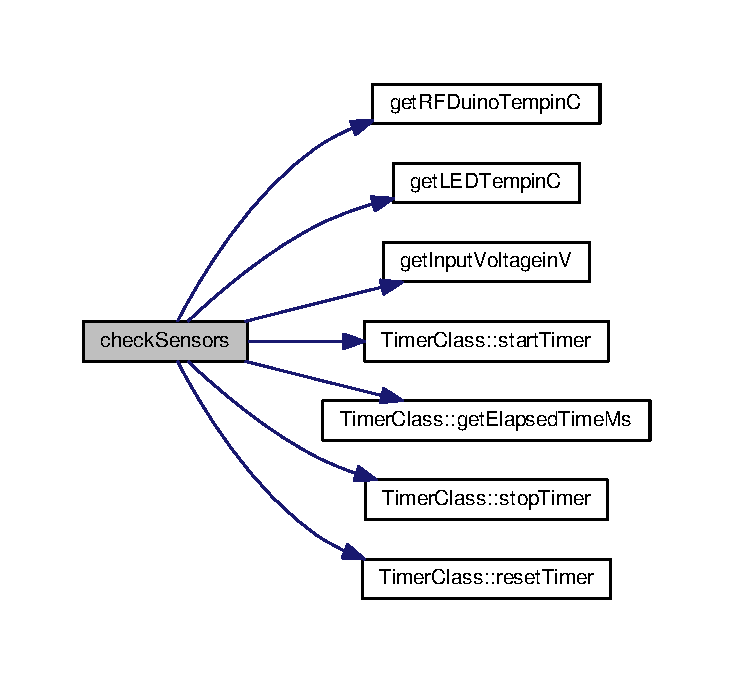
\includegraphics[width=350pt]{SensorManager_8h_ab791afb3dfb01137d61ffcc1a312ade5_cgraph}
\end{center}
\end{figure}




Here is the caller graph for this function\+:
\nopagebreak
\begin{figure}[H]
\begin{center}
\leavevmode
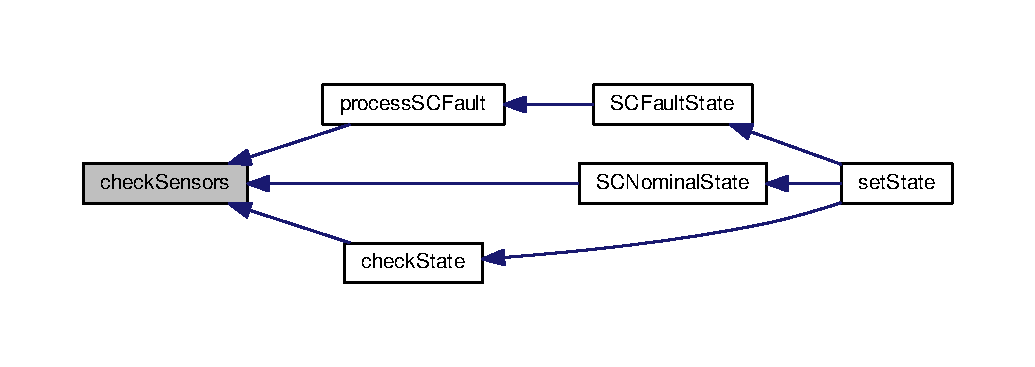
\includegraphics[width=350pt]{SensorManager_8h_ab791afb3dfb01137d61ffcc1a312ade5_icgraph}
\end{center}
\end{figure}


\index{Sensor\+Manager.\+h@{Sensor\+Manager.\+h}!get\+Input\+VoltageinmV@{get\+Input\+VoltageinmV}}
\index{get\+Input\+VoltageinmV@{get\+Input\+VoltageinmV}!Sensor\+Manager.\+h@{Sensor\+Manager.\+h}}
\subsubsection[{\texorpdfstring{get\+Input\+Voltageinm\+V(void)}{getInputVoltageinmV(void)}}]{\setlength{\rightskip}{0pt plus 5cm}int get\+Input\+VoltageinmV (
\begin{DoxyParamCaption}
\item[{void}]{}
\end{DoxyParamCaption}
)}\hypertarget{SensorManager_8h_aef3b6a94bf072b577b14b6bcdc1d6334}{}\label{SensorManager_8h_aef3b6a94bf072b577b14b6bcdc1d6334}
\index{Sensor\+Manager.\+h@{Sensor\+Manager.\+h}!get\+L\+E\+D\+TempinC@{get\+L\+E\+D\+TempinC}}
\index{get\+L\+E\+D\+TempinC@{get\+L\+E\+D\+TempinC}!Sensor\+Manager.\+h@{Sensor\+Manager.\+h}}
\subsubsection[{\texorpdfstring{get\+L\+E\+D\+Tempin\+C(void)}{getLEDTempinC(void)}}]{\setlength{\rightskip}{0pt plus 5cm}int get\+L\+E\+D\+TempinC (
\begin{DoxyParamCaption}
\item[{void}]{}
\end{DoxyParamCaption}
)}\hypertarget{SensorManager_8h_a1c943d491d2f32971f84a2eecdf00f2e}{}\label{SensorManager_8h_a1c943d491d2f32971f84a2eecdf00f2e}


Here is the caller graph for this function\+:
\nopagebreak
\begin{figure}[H]
\begin{center}
\leavevmode
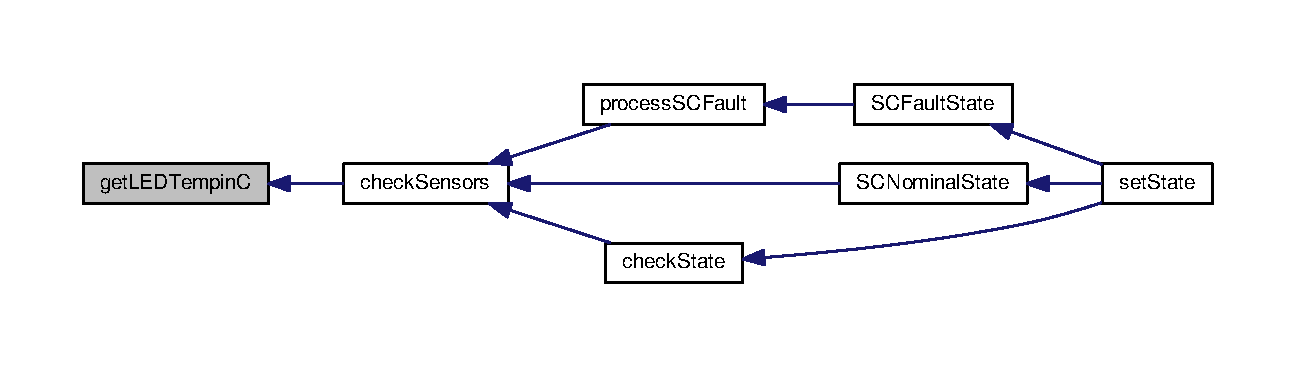
\includegraphics[width=350pt]{SensorManager_8h_a1c943d491d2f32971f84a2eecdf00f2e_icgraph}
\end{center}
\end{figure}


\index{Sensor\+Manager.\+h@{Sensor\+Manager.\+h}!get\+R\+F\+Duino\+TempinC@{get\+R\+F\+Duino\+TempinC}}
\index{get\+R\+F\+Duino\+TempinC@{get\+R\+F\+Duino\+TempinC}!Sensor\+Manager.\+h@{Sensor\+Manager.\+h}}
\subsubsection[{\texorpdfstring{get\+R\+F\+Duino\+Tempin\+C(void)}{getRFDuinoTempinC(void)}}]{\setlength{\rightskip}{0pt plus 5cm}int get\+R\+F\+Duino\+TempinC (
\begin{DoxyParamCaption}
\item[{void}]{}
\end{DoxyParamCaption}
)}\hypertarget{SensorManager_8h_a1b9f0e0ff57635f1e86c2c7fcddab439}{}\label{SensorManager_8h_a1b9f0e0ff57635f1e86c2c7fcddab439}


Here is the caller graph for this function\+:
\nopagebreak
\begin{figure}[H]
\begin{center}
\leavevmode
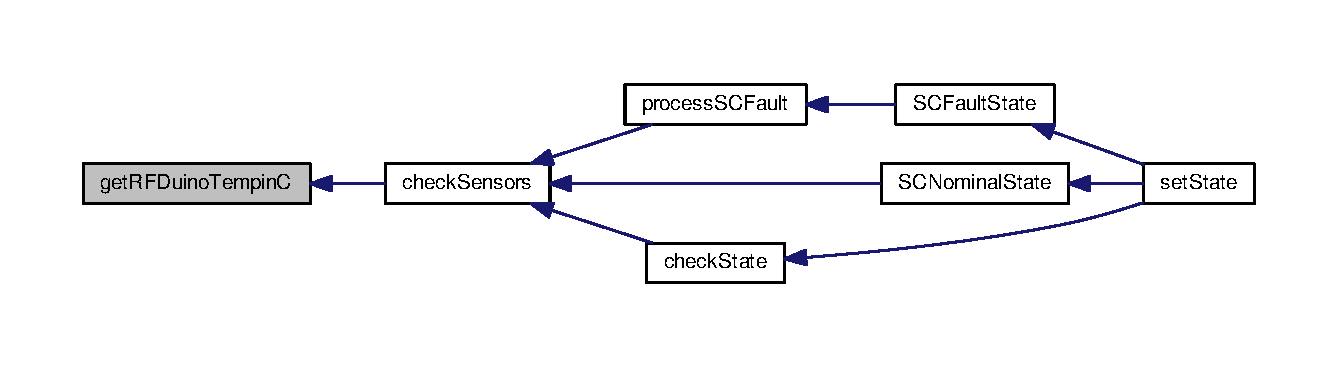
\includegraphics[width=350pt]{SensorManager_8h_a1b9f0e0ff57635f1e86c2c7fcddab439_icgraph}
\end{center}
\end{figure}




\subsection{Variable Documentation}
\index{Sensor\+Manager.\+h@{Sensor\+Manager.\+h}!sensor\+Feedback@{sensor\+Feedback}}
\index{sensor\+Feedback@{sensor\+Feedback}!Sensor\+Manager.\+h@{Sensor\+Manager.\+h}}
\subsubsection[{\texorpdfstring{sensor\+Feedback}{sensorFeedback}}]{\setlength{\rightskip}{0pt plus 5cm}{\bf sensor\+Feedback} {\bf sensor\+Feedback}}\hypertarget{SensorManager_8h_a28902247617a380eadc4313c5df4c270}{}\label{SensorManager_8h_a28902247617a380eadc4313c5df4c270}

\hypertarget{SerialDebug_8cpp}{}\section{Serial\+Debug.\+cpp File Reference}
\label{SerialDebug_8cpp}\index{Serial\+Debug.\+cpp@{Serial\+Debug.\+cpp}}
{\ttfamily \#include \char`\"{}Serial\+Debug.\+h\char`\"{}}\\*
Include dependency graph for Serial\+Debug.\+cpp\+:
\nopagebreak
\begin{figure}[H]
\begin{center}
\leavevmode
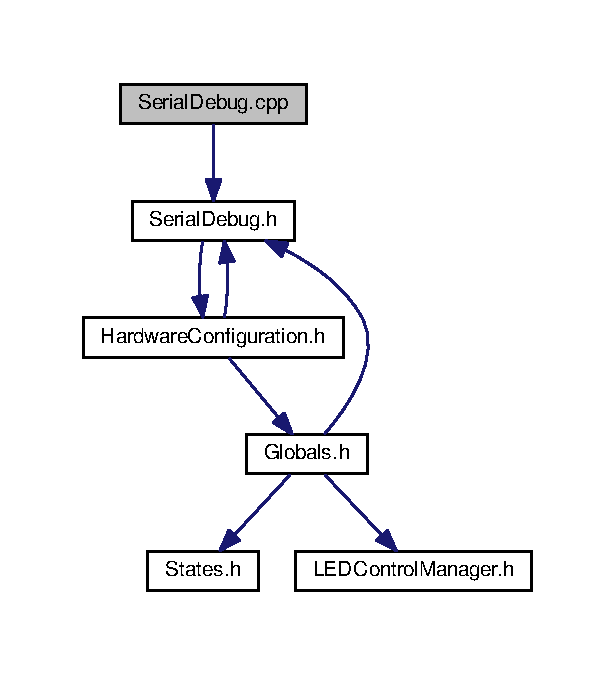
\includegraphics[width=295pt]{SerialDebug_8cpp__incl}
\end{center}
\end{figure}
\subsection*{Functions}
\begin{DoxyCompactItemize}
\item 
void \hyperlink{SerialDebug_8cpp_a31ea1e399090f7bf6edabad2905b4004}{check\+Serial} (void)
\item 
void \hyperlink{SerialDebug_8cpp_af2b53c59b5d16b731bf52803f697e536}{check\+Debug\+Send\+Time} (void)
\end{DoxyCompactItemize}
\subsection*{Variables}
\begin{DoxyCompactItemize}
\item 
enum \hyperlink{SerialDebug_8h_a2e1d76111dc436b8a6e003c74f4919f4}{Debug\+Levels} \hyperlink{SerialDebug_8cpp_a81f9a52045ef198ec20038a6b02aba35}{Serial\+Debug\+Level} = \hyperlink{SerialDebug_8h_a2e1d76111dc436b8a6e003c74f4919f4a7a352a3dd2accc1dd65a4538c3754ee8}{Low}
\end{DoxyCompactItemize}


\subsection{Function Documentation}
\index{Serial\+Debug.\+cpp@{Serial\+Debug.\+cpp}!check\+Debug\+Send\+Time@{check\+Debug\+Send\+Time}}
\index{check\+Debug\+Send\+Time@{check\+Debug\+Send\+Time}!Serial\+Debug.\+cpp@{Serial\+Debug.\+cpp}}
\subsubsection[{\texorpdfstring{check\+Debug\+Send\+Time(void)}{checkDebugSendTime(void)}}]{\setlength{\rightskip}{0pt plus 5cm}void check\+Debug\+Send\+Time (
\begin{DoxyParamCaption}
\item[{void}]{}
\end{DoxyParamCaption}
)}\hypertarget{SerialDebug_8cpp_af2b53c59b5d16b731bf52803f697e536}{}\label{SerialDebug_8cpp_af2b53c59b5d16b731bf52803f697e536}
\index{Serial\+Debug.\+cpp@{Serial\+Debug.\+cpp}!check\+Serial@{check\+Serial}}
\index{check\+Serial@{check\+Serial}!Serial\+Debug.\+cpp@{Serial\+Debug.\+cpp}}
\subsubsection[{\texorpdfstring{check\+Serial(void)}{checkSerial(void)}}]{\setlength{\rightskip}{0pt plus 5cm}void check\+Serial (
\begin{DoxyParamCaption}
\item[{void}]{}
\end{DoxyParamCaption}
)}\hypertarget{SerialDebug_8cpp_a31ea1e399090f7bf6edabad2905b4004}{}\label{SerialDebug_8cpp_a31ea1e399090f7bf6edabad2905b4004}


\subsection{Variable Documentation}
\index{Serial\+Debug.\+cpp@{Serial\+Debug.\+cpp}!Serial\+Debug\+Level@{Serial\+Debug\+Level}}
\index{Serial\+Debug\+Level@{Serial\+Debug\+Level}!Serial\+Debug.\+cpp@{Serial\+Debug.\+cpp}}
\subsubsection[{\texorpdfstring{Serial\+Debug\+Level}{SerialDebugLevel}}]{\setlength{\rightskip}{0pt plus 5cm}enum {\bf Debug\+Levels} Serial\+Debug\+Level = {\bf Low}}\hypertarget{SerialDebug_8cpp_a81f9a52045ef198ec20038a6b02aba35}{}\label{SerialDebug_8cpp_a81f9a52045ef198ec20038a6b02aba35}

\hypertarget{SerialDebug_8h}{}\section{Serial\+Debug.\+h File Reference}
\label{SerialDebug_8h}\index{Serial\+Debug.\+h@{Serial\+Debug.\+h}}
{\ttfamily \#include \char`\"{}Hardware\+Configuration.\+h\char`\"{}}\\*
Include dependency graph for Serial\+Debug.\+h\+:
\nopagebreak
\begin{figure}[H]
\begin{center}
\leavevmode
\includegraphics[width=295pt]{SerialDebug_8h__incl}
\end{center}
\end{figure}
This graph shows which files directly or indirectly include this file\+:
\nopagebreak
\begin{figure}[H]
\begin{center}
\leavevmode
\includegraphics[width=350pt]{SerialDebug_8h__dep__incl}
\end{center}
\end{figure}
\subsection*{Macros}
\begin{DoxyCompactItemize}
\item 
\#define \hyperlink{SerialDebug_8h_a04ed22e812ec03a8942c40bd6df5ff3b}{T\+E\+R\+M\+I\+N\+A\+L\+\_\+\+LF}~Serial.\+println
\item 
\#define \hyperlink{SerialDebug_8h_a5250b667cb28dd60b71e6e04e23eac37}{T\+E\+R\+M\+I\+N\+AL}~Serial.\+print
\item 
\#define \hyperlink{SerialDebug_8h_ac28b2f0cc0d8aabe8b3148d4a5cccc6d}{D\+E\+B\+U\+G\+\_\+\+LF}(level,  message)~if(Serial\+Debug\+Level!=\hyperlink{SerialDebug_8h_a2e1d76111dc436b8a6e003c74f4919f4ad8a892b94d3a94ea861543c085ae782b}{Off} \&\& level $<$= \hyperlink{SerialDebug_8h_a81f9a52045ef198ec20038a6b02aba35}{Serial\+Debug\+Level}) Serial.\+println(message)
\item 
\#define \hyperlink{SerialDebug_8h_a94c021eedec413719a519e8652592d41}{D\+E\+B\+UG}(level,  message)~if(Serial\+Debug\+Level!=\hyperlink{SerialDebug_8h_a2e1d76111dc436b8a6e003c74f4919f4ad8a892b94d3a94ea861543c085ae782b}{Off} \&\& level $<$= \hyperlink{SerialDebug_8h_a81f9a52045ef198ec20038a6b02aba35}{Serial\+Debug\+Level}) Serial.\+print(message)
\item 
\#define \hyperlink{SerialDebug_8h_a0ef4c095f19f348a7e65acabf9848f72}{T\+I\+M\+E\+D\+\_\+\+D\+E\+B\+UG}~if(\hyperlink{structFlashMemoryData_aa5ccce295f4c2cf838962fbfca9ee9a9}{Flash\+Memory\+Data.\+data\+Refresh\+Time\+Met})
\end{DoxyCompactItemize}
\subsection*{Enumerations}
\begin{DoxyCompactItemize}
\item 
enum \hyperlink{SerialDebug_8h_a2e1d76111dc436b8a6e003c74f4919f4}{Debug\+Levels} \{ \\*
\hyperlink{SerialDebug_8h_a2e1d76111dc436b8a6e003c74f4919f4ad8a892b94d3a94ea861543c085ae782b}{Off}, 
\hyperlink{SerialDebug_8h_a2e1d76111dc436b8a6e003c74f4919f4afd04aa7a2a2337eff410dbde4b4598ce}{Sensor}, 
\hyperlink{SerialDebug_8h_a2e1d76111dc436b8a6e003c74f4919f4a7a352a3dd2accc1dd65a4538c3754ee8}{Low}, 
\hyperlink{SerialDebug_8h_a2e1d76111dc436b8a6e003c74f4919f4a8cfb9311a439a51b14159ed0970f398b}{Medium}, 
\\*
\hyperlink{SerialDebug_8h_a2e1d76111dc436b8a6e003c74f4919f4a24c57acd029e3f96fede49402ea01e6f}{High}
 \}
\end{DoxyCompactItemize}
\subsection*{Functions}
\begin{DoxyCompactItemize}
\item 
void \hyperlink{SerialDebug_8h_a31ea1e399090f7bf6edabad2905b4004}{check\+Serial} (void)
\item 
void \hyperlink{SerialDebug_8h_af2b53c59b5d16b731bf52803f697e536}{check\+Debug\+Send\+Time} (void)
\end{DoxyCompactItemize}
\subsection*{Variables}
\begin{DoxyCompactItemize}
\item 
enum \hyperlink{SerialDebug_8h_a2e1d76111dc436b8a6e003c74f4919f4}{Debug\+Levels} \hyperlink{SerialDebug_8h_a81f9a52045ef198ec20038a6b02aba35}{Serial\+Debug\+Level}
\end{DoxyCompactItemize}


\subsection{Macro Definition Documentation}
\index{Serial\+Debug.\+h@{Serial\+Debug.\+h}!D\+E\+B\+UG@{D\+E\+B\+UG}}
\index{D\+E\+B\+UG@{D\+E\+B\+UG}!Serial\+Debug.\+h@{Serial\+Debug.\+h}}
\subsubsection[{\texorpdfstring{D\+E\+B\+UG}{DEBUG}}]{\setlength{\rightskip}{0pt plus 5cm}\#define D\+E\+B\+UG(
\begin{DoxyParamCaption}
\item[{}]{level, }
\item[{}]{message}
\end{DoxyParamCaption}
)~if(Serial\+Debug\+Level!={\bf Off} \&\& level $<$= {\bf Serial\+Debug\+Level}) Serial.\+print(message)}\hypertarget{SerialDebug_8h_a94c021eedec413719a519e8652592d41}{}\label{SerialDebug_8h_a94c021eedec413719a519e8652592d41}
\index{Serial\+Debug.\+h@{Serial\+Debug.\+h}!D\+E\+B\+U\+G\+\_\+\+LF@{D\+E\+B\+U\+G\+\_\+\+LF}}
\index{D\+E\+B\+U\+G\+\_\+\+LF@{D\+E\+B\+U\+G\+\_\+\+LF}!Serial\+Debug.\+h@{Serial\+Debug.\+h}}
\subsubsection[{\texorpdfstring{D\+E\+B\+U\+G\+\_\+\+LF}{DEBUG_LF}}]{\setlength{\rightskip}{0pt plus 5cm}\#define D\+E\+B\+U\+G\+\_\+\+LF(
\begin{DoxyParamCaption}
\item[{}]{level, }
\item[{}]{message}
\end{DoxyParamCaption}
)~if(Serial\+Debug\+Level!={\bf Off} \&\& level $<$= {\bf Serial\+Debug\+Level}) Serial.\+println(message)}\hypertarget{SerialDebug_8h_ac28b2f0cc0d8aabe8b3148d4a5cccc6d}{}\label{SerialDebug_8h_ac28b2f0cc0d8aabe8b3148d4a5cccc6d}
\index{Serial\+Debug.\+h@{Serial\+Debug.\+h}!T\+E\+R\+M\+I\+N\+AL@{T\+E\+R\+M\+I\+N\+AL}}
\index{T\+E\+R\+M\+I\+N\+AL@{T\+E\+R\+M\+I\+N\+AL}!Serial\+Debug.\+h@{Serial\+Debug.\+h}}
\subsubsection[{\texorpdfstring{T\+E\+R\+M\+I\+N\+AL}{TERMINAL}}]{\setlength{\rightskip}{0pt plus 5cm}\#define T\+E\+R\+M\+I\+N\+AL~Serial.\+print}\hypertarget{SerialDebug_8h_a5250b667cb28dd60b71e6e04e23eac37}{}\label{SerialDebug_8h_a5250b667cb28dd60b71e6e04e23eac37}
\index{Serial\+Debug.\+h@{Serial\+Debug.\+h}!T\+E\+R\+M\+I\+N\+A\+L\+\_\+\+LF@{T\+E\+R\+M\+I\+N\+A\+L\+\_\+\+LF}}
\index{T\+E\+R\+M\+I\+N\+A\+L\+\_\+\+LF@{T\+E\+R\+M\+I\+N\+A\+L\+\_\+\+LF}!Serial\+Debug.\+h@{Serial\+Debug.\+h}}
\subsubsection[{\texorpdfstring{T\+E\+R\+M\+I\+N\+A\+L\+\_\+\+LF}{TERMINAL_LF}}]{\setlength{\rightskip}{0pt plus 5cm}\#define T\+E\+R\+M\+I\+N\+A\+L\+\_\+\+LF~Serial.\+println}\hypertarget{SerialDebug_8h_a04ed22e812ec03a8942c40bd6df5ff3b}{}\label{SerialDebug_8h_a04ed22e812ec03a8942c40bd6df5ff3b}
\index{Serial\+Debug.\+h@{Serial\+Debug.\+h}!T\+I\+M\+E\+D\+\_\+\+D\+E\+B\+UG@{T\+I\+M\+E\+D\+\_\+\+D\+E\+B\+UG}}
\index{T\+I\+M\+E\+D\+\_\+\+D\+E\+B\+UG@{T\+I\+M\+E\+D\+\_\+\+D\+E\+B\+UG}!Serial\+Debug.\+h@{Serial\+Debug.\+h}}
\subsubsection[{\texorpdfstring{T\+I\+M\+E\+D\+\_\+\+D\+E\+B\+UG}{TIMED_DEBUG}}]{\setlength{\rightskip}{0pt plus 5cm}\#define T\+I\+M\+E\+D\+\_\+\+D\+E\+B\+UG~if({\bf Flash\+Memory\+Data.\+data\+Refresh\+Time\+Met})}\hypertarget{SerialDebug_8h_a0ef4c095f19f348a7e65acabf9848f72}{}\label{SerialDebug_8h_a0ef4c095f19f348a7e65acabf9848f72}


\subsection{Enumeration Type Documentation}
\index{Serial\+Debug.\+h@{Serial\+Debug.\+h}!Debug\+Levels@{Debug\+Levels}}
\index{Debug\+Levels@{Debug\+Levels}!Serial\+Debug.\+h@{Serial\+Debug.\+h}}
\subsubsection[{\texorpdfstring{Debug\+Levels}{DebugLevels}}]{\setlength{\rightskip}{0pt plus 5cm}enum {\bf Debug\+Levels}}\hypertarget{SerialDebug_8h_a2e1d76111dc436b8a6e003c74f4919f4}{}\label{SerialDebug_8h_a2e1d76111dc436b8a6e003c74f4919f4}
\begin{Desc}
\item[Enumerator]\par
\begin{description}
\index{Off@{Off}!Serial\+Debug.\+h@{Serial\+Debug.\+h}}\index{Serial\+Debug.\+h@{Serial\+Debug.\+h}!Off@{Off}}\item[{\em 
Off\hypertarget{SerialDebug_8h_a2e1d76111dc436b8a6e003c74f4919f4ad8a892b94d3a94ea861543c085ae782b}{}\label{SerialDebug_8h_a2e1d76111dc436b8a6e003c74f4919f4ad8a892b94d3a94ea861543c085ae782b}
}]\index{Sensor@{Sensor}!Serial\+Debug.\+h@{Serial\+Debug.\+h}}\index{Serial\+Debug.\+h@{Serial\+Debug.\+h}!Sensor@{Sensor}}\item[{\em 
Sensor\hypertarget{SerialDebug_8h_a2e1d76111dc436b8a6e003c74f4919f4afd04aa7a2a2337eff410dbde4b4598ce}{}\label{SerialDebug_8h_a2e1d76111dc436b8a6e003c74f4919f4afd04aa7a2a2337eff410dbde4b4598ce}
}]\index{Low@{Low}!Serial\+Debug.\+h@{Serial\+Debug.\+h}}\index{Serial\+Debug.\+h@{Serial\+Debug.\+h}!Low@{Low}}\item[{\em 
Low\hypertarget{SerialDebug_8h_a2e1d76111dc436b8a6e003c74f4919f4a7a352a3dd2accc1dd65a4538c3754ee8}{}\label{SerialDebug_8h_a2e1d76111dc436b8a6e003c74f4919f4a7a352a3dd2accc1dd65a4538c3754ee8}
}]\index{Medium@{Medium}!Serial\+Debug.\+h@{Serial\+Debug.\+h}}\index{Serial\+Debug.\+h@{Serial\+Debug.\+h}!Medium@{Medium}}\item[{\em 
Medium\hypertarget{SerialDebug_8h_a2e1d76111dc436b8a6e003c74f4919f4a8cfb9311a439a51b14159ed0970f398b}{}\label{SerialDebug_8h_a2e1d76111dc436b8a6e003c74f4919f4a8cfb9311a439a51b14159ed0970f398b}
}]\index{High@{High}!Serial\+Debug.\+h@{Serial\+Debug.\+h}}\index{Serial\+Debug.\+h@{Serial\+Debug.\+h}!High@{High}}\item[{\em 
High\hypertarget{SerialDebug_8h_a2e1d76111dc436b8a6e003c74f4919f4a24c57acd029e3f96fede49402ea01e6f}{}\label{SerialDebug_8h_a2e1d76111dc436b8a6e003c74f4919f4a24c57acd029e3f96fede49402ea01e6f}
}]\end{description}
\end{Desc}


\subsection{Function Documentation}
\index{Serial\+Debug.\+h@{Serial\+Debug.\+h}!check\+Debug\+Send\+Time@{check\+Debug\+Send\+Time}}
\index{check\+Debug\+Send\+Time@{check\+Debug\+Send\+Time}!Serial\+Debug.\+h@{Serial\+Debug.\+h}}
\subsubsection[{\texorpdfstring{check\+Debug\+Send\+Time(void)}{checkDebugSendTime(void)}}]{\setlength{\rightskip}{0pt plus 5cm}void check\+Debug\+Send\+Time (
\begin{DoxyParamCaption}
\item[{void}]{}
\end{DoxyParamCaption}
)}\hypertarget{SerialDebug_8h_af2b53c59b5d16b731bf52803f697e536}{}\label{SerialDebug_8h_af2b53c59b5d16b731bf52803f697e536}
\index{Serial\+Debug.\+h@{Serial\+Debug.\+h}!check\+Serial@{check\+Serial}}
\index{check\+Serial@{check\+Serial}!Serial\+Debug.\+h@{Serial\+Debug.\+h}}
\subsubsection[{\texorpdfstring{check\+Serial(void)}{checkSerial(void)}}]{\setlength{\rightskip}{0pt plus 5cm}void check\+Serial (
\begin{DoxyParamCaption}
\item[{void}]{}
\end{DoxyParamCaption}
)}\hypertarget{SerialDebug_8h_a31ea1e399090f7bf6edabad2905b4004}{}\label{SerialDebug_8h_a31ea1e399090f7bf6edabad2905b4004}


\subsection{Variable Documentation}
\index{Serial\+Debug.\+h@{Serial\+Debug.\+h}!Serial\+Debug\+Level@{Serial\+Debug\+Level}}
\index{Serial\+Debug\+Level@{Serial\+Debug\+Level}!Serial\+Debug.\+h@{Serial\+Debug.\+h}}
\subsubsection[{\texorpdfstring{Serial\+Debug\+Level}{SerialDebugLevel}}]{\setlength{\rightskip}{0pt plus 5cm}enum {\bf Debug\+Levels} Serial\+Debug\+Level}\hypertarget{SerialDebug_8h_a81f9a52045ef198ec20038a6b02aba35}{}\label{SerialDebug_8h_a81f9a52045ef198ec20038a6b02aba35}

\hypertarget{States_8cpp}{}\section{States.\+cpp File Reference}
\label{States_8cpp}\index{States.\+cpp@{States.\+cpp}}
{\ttfamily \#include \char`\"{}States.\+h\char`\"{}}\\*
{\ttfamily \#include $<$Arduino.\+h$>$}\\*
{\ttfamily \#include $<$string.\+h$>$}\\*
{\ttfamily \#include \char`\"{}Pin\+Definitions.\+h\char`\"{}}\\*
{\ttfamily \#include \char`\"{}L\+E\+D\+Control\+Manager.\+h\char`\"{}}\\*
{\ttfamily \#include \char`\"{}Globals.\+h\char`\"{}}\\*
{\ttfamily \#include \char`\"{}Sensor\+Manager.\+h\char`\"{}}\\*
{\ttfamily \#include \char`\"{}Hardware\+Configuration.\+h\char`\"{}}\\*
{\ttfamily \#include \char`\"{}Serial\+Debug.\+h\char`\"{}}\\*
{\ttfamily \#include \char`\"{}Fault\+Handler.\+h\char`\"{}}\\*
Include dependency graph for States.\+cpp\+:
\nopagebreak
\begin{figure}[H]
\begin{center}
\leavevmode
\includegraphics[width=350pt]{States_8cpp__incl}
\end{center}
\end{figure}
\subsection*{Functions}
\begin{DoxyCompactItemize}
\item 
void \hyperlink{States_8cpp_a88e12751e4ec18de911d1a6a370394fd}{configure\+Pins} (void)
\item 
void \hyperlink{States_8cpp_a19ebe9f470610e6867c7f4724aa5da9b}{initialize\+System} (void)
\item 
void \hyperlink{States_8cpp_a003b78d5f813ae024018e90b3f67616d}{print\+Start\+Up\+Data} (void)
\item 
void \hyperlink{States_8cpp_abbe8f188b5d7ee5d6e0f1c8ab7fbaf35}{check\+Boot\+Complete} (void)
\item 
void \hyperlink{States_8cpp_a014eac3f1950f3311061d95e6240e35e}{S\+C\+Nominal\+State} (void)
\item 
void \hyperlink{States_8cpp_a97ec32d4f361a6ccb14d50c278bd8918}{S\+C\+Fault\+State} (void)
\item 
\hyperlink{States_8h_a808e5cd4979462d3bbe3070d7d147444}{States} \hyperlink{States_8cpp_a94a0a3dea0a4d6e139048a509e9af485}{check\+State} (void)
\item 
void \hyperlink{States_8cpp_a4ff66e43394ec663d13535ac7f85b9d3}{set\+State} (void)
\end{DoxyCompactItemize}
\subsection*{Variables}
\begin{DoxyCompactItemize}
\item 
static bool \hyperlink{States_8cpp_a51bb69959c09a95251821128ff1a5438}{new\+State\+Print\+Flag} = false
\item 
class \hyperlink{classTimerClass}{Timer\+Class} \hyperlink{States_8cpp_a3fcdf9051c7095d731ae965a81a516d3}{Startup\+Timer}
\end{DoxyCompactItemize}


\subsection{Function Documentation}
\index{States.\+cpp@{States.\+cpp}!check\+Boot\+Complete@{check\+Boot\+Complete}}
\index{check\+Boot\+Complete@{check\+Boot\+Complete}!States.\+cpp@{States.\+cpp}}
\subsubsection[{\texorpdfstring{check\+Boot\+Complete(void)}{checkBootComplete(void)}}]{\setlength{\rightskip}{0pt plus 5cm}void check\+Boot\+Complete (
\begin{DoxyParamCaption}
\item[{void}]{}
\end{DoxyParamCaption}
)}\hypertarget{States_8cpp_abbe8f188b5d7ee5d6e0f1c8ab7fbaf35}{}\label{States_8cpp_abbe8f188b5d7ee5d6e0f1c8ab7fbaf35}


Here is the call graph for this function\+:
\nopagebreak
\begin{figure}[H]
\begin{center}
\leavevmode
\includegraphics[width=311pt]{States_8cpp_abbe8f188b5d7ee5d6e0f1c8ab7fbaf35_cgraph}
\end{center}
\end{figure}


\index{States.\+cpp@{States.\+cpp}!check\+State@{check\+State}}
\index{check\+State@{check\+State}!States.\+cpp@{States.\+cpp}}
\subsubsection[{\texorpdfstring{check\+State(void)}{checkState(void)}}]{\setlength{\rightskip}{0pt plus 5cm}{\bf States} check\+State (
\begin{DoxyParamCaption}
\item[{void}]{}
\end{DoxyParamCaption}
)}\hypertarget{States_8cpp_a94a0a3dea0a4d6e139048a509e9af485}{}\label{States_8cpp_a94a0a3dea0a4d6e139048a509e9af485}


Here is the call graph for this function\+:
\nopagebreak
\begin{figure}[H]
\begin{center}
\leavevmode
\includegraphics[width=350pt]{States_8cpp_a94a0a3dea0a4d6e139048a509e9af485_cgraph}
\end{center}
\end{figure}




Here is the caller graph for this function\+:
\nopagebreak
\begin{figure}[H]
\begin{center}
\leavevmode
\includegraphics[width=235pt]{States_8cpp_a94a0a3dea0a4d6e139048a509e9af485_icgraph}
\end{center}
\end{figure}


\index{States.\+cpp@{States.\+cpp}!configure\+Pins@{configure\+Pins}}
\index{configure\+Pins@{configure\+Pins}!States.\+cpp@{States.\+cpp}}
\subsubsection[{\texorpdfstring{configure\+Pins(void)}{configurePins(void)}}]{\setlength{\rightskip}{0pt plus 5cm}void configure\+Pins (
\begin{DoxyParamCaption}
\item[{void}]{}
\end{DoxyParamCaption}
)}\hypertarget{States_8cpp_a88e12751e4ec18de911d1a6a370394fd}{}\label{States_8cpp_a88e12751e4ec18de911d1a6a370394fd}


Here is the caller graph for this function\+:
\nopagebreak
\begin{figure}[H]
\begin{center}
\leavevmode
\includegraphics[width=278pt]{States_8cpp_a88e12751e4ec18de911d1a6a370394fd_icgraph}
\end{center}
\end{figure}


\index{States.\+cpp@{States.\+cpp}!initialize\+System@{initialize\+System}}
\index{initialize\+System@{initialize\+System}!States.\+cpp@{States.\+cpp}}
\subsubsection[{\texorpdfstring{initialize\+System(void)}{initializeSystem(void)}}]{\setlength{\rightskip}{0pt plus 5cm}void initialize\+System (
\begin{DoxyParamCaption}
\item[{void}]{}
\end{DoxyParamCaption}
)}\hypertarget{States_8cpp_a19ebe9f470610e6867c7f4724aa5da9b}{}\label{States_8cpp_a19ebe9f470610e6867c7f4724aa5da9b}


Here is the call graph for this function\+:
\nopagebreak
\begin{figure}[H]
\begin{center}
\leavevmode
\includegraphics[width=350pt]{States_8cpp_a19ebe9f470610e6867c7f4724aa5da9b_cgraph}
\end{center}
\end{figure}


\index{States.\+cpp@{States.\+cpp}!print\+Start\+Up\+Data@{print\+Start\+Up\+Data}}
\index{print\+Start\+Up\+Data@{print\+Start\+Up\+Data}!States.\+cpp@{States.\+cpp}}
\subsubsection[{\texorpdfstring{print\+Start\+Up\+Data(void)}{printStartUpData(void)}}]{\setlength{\rightskip}{0pt plus 5cm}void print\+Start\+Up\+Data (
\begin{DoxyParamCaption}
\item[{void}]{}
\end{DoxyParamCaption}
)}\hypertarget{States_8cpp_a003b78d5f813ae024018e90b3f67616d}{}\label{States_8cpp_a003b78d5f813ae024018e90b3f67616d}


Here is the caller graph for this function\+:
\nopagebreak
\begin{figure}[H]
\begin{center}
\leavevmode
\includegraphics[width=311pt]{States_8cpp_a003b78d5f813ae024018e90b3f67616d_icgraph}
\end{center}
\end{figure}


\index{States.\+cpp@{States.\+cpp}!S\+C\+Fault\+State@{S\+C\+Fault\+State}}
\index{S\+C\+Fault\+State@{S\+C\+Fault\+State}!States.\+cpp@{States.\+cpp}}
\subsubsection[{\texorpdfstring{S\+C\+Fault\+State(void)}{SCFaultState(void)}}]{\setlength{\rightskip}{0pt plus 5cm}void S\+C\+Fault\+State (
\begin{DoxyParamCaption}
\item[{void}]{}
\end{DoxyParamCaption}
)}\hypertarget{States_8cpp_a97ec32d4f361a6ccb14d50c278bd8918}{}\label{States_8cpp_a97ec32d4f361a6ccb14d50c278bd8918}


Here is the call graph for this function\+:
\nopagebreak
\begin{figure}[H]
\begin{center}
\leavevmode
\includegraphics[width=350pt]{States_8cpp_a97ec32d4f361a6ccb14d50c278bd8918_cgraph}
\end{center}
\end{figure}




Here is the caller graph for this function\+:
\nopagebreak
\begin{figure}[H]
\begin{center}
\leavevmode
\includegraphics[width=245pt]{States_8cpp_a97ec32d4f361a6ccb14d50c278bd8918_icgraph}
\end{center}
\end{figure}


\index{States.\+cpp@{States.\+cpp}!S\+C\+Nominal\+State@{S\+C\+Nominal\+State}}
\index{S\+C\+Nominal\+State@{S\+C\+Nominal\+State}!States.\+cpp@{States.\+cpp}}
\subsubsection[{\texorpdfstring{S\+C\+Nominal\+State(void)}{SCNominalState(void)}}]{\setlength{\rightskip}{0pt plus 5cm}void S\+C\+Nominal\+State (
\begin{DoxyParamCaption}
\item[{void}]{}
\end{DoxyParamCaption}
)}\hypertarget{States_8cpp_a014eac3f1950f3311061d95e6240e35e}{}\label{States_8cpp_a014eac3f1950f3311061d95e6240e35e}


Here is the call graph for this function\+:
\nopagebreak
\begin{figure}[H]
\begin{center}
\leavevmode
\includegraphics[width=350pt]{States_8cpp_a014eac3f1950f3311061d95e6240e35e_cgraph}
\end{center}
\end{figure}




Here is the caller graph for this function\+:
\nopagebreak
\begin{figure}[H]
\begin{center}
\leavevmode
\includegraphics[width=259pt]{States_8cpp_a014eac3f1950f3311061d95e6240e35e_icgraph}
\end{center}
\end{figure}


\index{States.\+cpp@{States.\+cpp}!set\+State@{set\+State}}
\index{set\+State@{set\+State}!States.\+cpp@{States.\+cpp}}
\subsubsection[{\texorpdfstring{set\+State(void)}{setState(void)}}]{\setlength{\rightskip}{0pt plus 5cm}void set\+State (
\begin{DoxyParamCaption}
\item[{void}]{}
\end{DoxyParamCaption}
)}\hypertarget{States_8cpp_a4ff66e43394ec663d13535ac7f85b9d3}{}\label{States_8cpp_a4ff66e43394ec663d13535ac7f85b9d3}


Here is the call graph for this function\+:
\nopagebreak
\begin{figure}[H]
\begin{center}
\leavevmode
\includegraphics[width=350pt]{States_8cpp_a4ff66e43394ec663d13535ac7f85b9d3_cgraph}
\end{center}
\end{figure}




\subsection{Variable Documentation}
\index{States.\+cpp@{States.\+cpp}!new\+State\+Print\+Flag@{new\+State\+Print\+Flag}}
\index{new\+State\+Print\+Flag@{new\+State\+Print\+Flag}!States.\+cpp@{States.\+cpp}}
\subsubsection[{\texorpdfstring{new\+State\+Print\+Flag}{newStatePrintFlag}}]{\setlength{\rightskip}{0pt plus 5cm}bool new\+State\+Print\+Flag = false\hspace{0.3cm}{\ttfamily [static]}}\hypertarget{States_8cpp_a51bb69959c09a95251821128ff1a5438}{}\label{States_8cpp_a51bb69959c09a95251821128ff1a5438}
\index{States.\+cpp@{States.\+cpp}!Startup\+Timer@{Startup\+Timer}}
\index{Startup\+Timer@{Startup\+Timer}!States.\+cpp@{States.\+cpp}}
\subsubsection[{\texorpdfstring{Startup\+Timer}{StartupTimer}}]{\setlength{\rightskip}{0pt plus 5cm}class {\bf Timer\+Class} Startup\+Timer}\hypertarget{States_8cpp_a3fcdf9051c7095d731ae965a81a516d3}{}\label{States_8cpp_a3fcdf9051c7095d731ae965a81a516d3}

\hypertarget{States_8h}{}\section{States.\+h File Reference}
\label{States_8h}\index{States.\+h@{States.\+h}}
This graph shows which files directly or indirectly include this file\+:
\nopagebreak
\begin{figure}[H]
\begin{center}
\leavevmode
\includegraphics[width=350pt]{States_8h__dep__incl}
\end{center}
\end{figure}
\subsection*{Enumerations}
\begin{DoxyCompactItemize}
\item 
enum \hyperlink{States_8h_a808e5cd4979462d3bbe3070d7d147444}{States} \{ \\*
\hyperlink{States_8h_a808e5cd4979462d3bbe3070d7d147444a96e0c52c324ad0975fdd194f7dcaef5b}{R\+G\+B\+\_\+\+Disconnected}, 
\hyperlink{States_8h_a808e5cd4979462d3bbe3070d7d147444acfdfac3fe3a3d16a4402bd4b5a1a1bae}{R\+G\+B\+\_\+\+Connected}, 
\hyperlink{States_8h_a808e5cd4979462d3bbe3070d7d147444a2e47817ed677275f0ba1c665f610faa3}{R\+G\+B\+\_\+\+Fault}, 
\hyperlink{States_8h_a808e5cd4979462d3bbe3070d7d147444aae80d1b70b2876bf838a560703e4920d}{S\+C\+\_\+\+Nominal}, 
\\*
\hyperlink{States_8h_a808e5cd4979462d3bbe3070d7d147444afb4ff030e43dfdca8d6d5bf8417df529}{S\+C\+\_\+\+Fault}, 
\hyperlink{States_8h_a808e5cd4979462d3bbe3070d7d147444a1e36dd5b51c468e33bcf160523d402a7}{Boot}
 \}
\end{DoxyCompactItemize}
\subsection*{Functions}
\begin{DoxyCompactItemize}
\item 
void \hyperlink{States_8h_acaf637afd0683b349d523ddc12ee65bd}{on\+Radio\+Connect} (void)
\item 
void \hyperlink{States_8h_a0cb8e1ac67bc4d1ca7c9950caf334d14}{on\+Radio\+Disconnect} (void)
\item 
void \hyperlink{States_8h_a88e12751e4ec18de911d1a6a370394fd}{configure\+Pins} (void)
\item 
void \hyperlink{States_8h_a19ebe9f470610e6867c7f4724aa5da9b}{initialize\+System} (void)
\item 
void \hyperlink{States_8h_a003b78d5f813ae024018e90b3f67616d}{print\+Start\+Up\+Data} (void)
\item 
void \hyperlink{States_8h_abbe8f188b5d7ee5d6e0f1c8ab7fbaf35}{check\+Boot\+Complete} (void)
\item 
void \hyperlink{States_8h_a4ff66e43394ec663d13535ac7f85b9d3}{set\+State} (void)
\end{DoxyCompactItemize}


\subsection{Enumeration Type Documentation}
\index{States.\+h@{States.\+h}!States@{States}}
\index{States@{States}!States.\+h@{States.\+h}}
\subsubsection[{\texorpdfstring{States}{States}}]{\setlength{\rightskip}{0pt plus 5cm}enum {\bf States}}\hypertarget{States_8h_a808e5cd4979462d3bbe3070d7d147444}{}\label{States_8h_a808e5cd4979462d3bbe3070d7d147444}
\begin{Desc}
\item[Enumerator]\par
\begin{description}
\index{R\+G\+B\+\_\+\+Disconnected@{R\+G\+B\+\_\+\+Disconnected}!States.\+h@{States.\+h}}\index{States.\+h@{States.\+h}!R\+G\+B\+\_\+\+Disconnected@{R\+G\+B\+\_\+\+Disconnected}}\item[{\em 
R\+G\+B\+\_\+\+Disconnected\hypertarget{States_8h_a808e5cd4979462d3bbe3070d7d147444a96e0c52c324ad0975fdd194f7dcaef5b}{}\label{States_8h_a808e5cd4979462d3bbe3070d7d147444a96e0c52c324ad0975fdd194f7dcaef5b}
}]\index{R\+G\+B\+\_\+\+Connected@{R\+G\+B\+\_\+\+Connected}!States.\+h@{States.\+h}}\index{States.\+h@{States.\+h}!R\+G\+B\+\_\+\+Connected@{R\+G\+B\+\_\+\+Connected}}\item[{\em 
R\+G\+B\+\_\+\+Connected\hypertarget{States_8h_a808e5cd4979462d3bbe3070d7d147444acfdfac3fe3a3d16a4402bd4b5a1a1bae}{}\label{States_8h_a808e5cd4979462d3bbe3070d7d147444acfdfac3fe3a3d16a4402bd4b5a1a1bae}
}]\index{R\+G\+B\+\_\+\+Fault@{R\+G\+B\+\_\+\+Fault}!States.\+h@{States.\+h}}\index{States.\+h@{States.\+h}!R\+G\+B\+\_\+\+Fault@{R\+G\+B\+\_\+\+Fault}}\item[{\em 
R\+G\+B\+\_\+\+Fault\hypertarget{States_8h_a808e5cd4979462d3bbe3070d7d147444a2e47817ed677275f0ba1c665f610faa3}{}\label{States_8h_a808e5cd4979462d3bbe3070d7d147444a2e47817ed677275f0ba1c665f610faa3}
}]\index{S\+C\+\_\+\+Nominal@{S\+C\+\_\+\+Nominal}!States.\+h@{States.\+h}}\index{States.\+h@{States.\+h}!S\+C\+\_\+\+Nominal@{S\+C\+\_\+\+Nominal}}\item[{\em 
S\+C\+\_\+\+Nominal\hypertarget{States_8h_a808e5cd4979462d3bbe3070d7d147444aae80d1b70b2876bf838a560703e4920d}{}\label{States_8h_a808e5cd4979462d3bbe3070d7d147444aae80d1b70b2876bf838a560703e4920d}
}]\index{S\+C\+\_\+\+Fault@{S\+C\+\_\+\+Fault}!States.\+h@{States.\+h}}\index{States.\+h@{States.\+h}!S\+C\+\_\+\+Fault@{S\+C\+\_\+\+Fault}}\item[{\em 
S\+C\+\_\+\+Fault\hypertarget{States_8h_a808e5cd4979462d3bbe3070d7d147444afb4ff030e43dfdca8d6d5bf8417df529}{}\label{States_8h_a808e5cd4979462d3bbe3070d7d147444afb4ff030e43dfdca8d6d5bf8417df529}
}]\index{Boot@{Boot}!States.\+h@{States.\+h}}\index{States.\+h@{States.\+h}!Boot@{Boot}}\item[{\em 
Boot\hypertarget{States_8h_a808e5cd4979462d3bbe3070d7d147444a1e36dd5b51c468e33bcf160523d402a7}{}\label{States_8h_a808e5cd4979462d3bbe3070d7d147444a1e36dd5b51c468e33bcf160523d402a7}
}]\end{description}
\end{Desc}


\subsection{Function Documentation}
\index{States.\+h@{States.\+h}!check\+Boot\+Complete@{check\+Boot\+Complete}}
\index{check\+Boot\+Complete@{check\+Boot\+Complete}!States.\+h@{States.\+h}}
\subsubsection[{\texorpdfstring{check\+Boot\+Complete(void)}{checkBootComplete(void)}}]{\setlength{\rightskip}{0pt plus 5cm}void check\+Boot\+Complete (
\begin{DoxyParamCaption}
\item[{void}]{}
\end{DoxyParamCaption}
)}\hypertarget{States_8h_abbe8f188b5d7ee5d6e0f1c8ab7fbaf35}{}\label{States_8h_abbe8f188b5d7ee5d6e0f1c8ab7fbaf35}


Here is the call graph for this function\+:
\nopagebreak
\begin{figure}[H]
\begin{center}
\leavevmode
\includegraphics[width=311pt]{States_8h_abbe8f188b5d7ee5d6e0f1c8ab7fbaf35_cgraph}
\end{center}
\end{figure}


\index{States.\+h@{States.\+h}!configure\+Pins@{configure\+Pins}}
\index{configure\+Pins@{configure\+Pins}!States.\+h@{States.\+h}}
\subsubsection[{\texorpdfstring{configure\+Pins(void)}{configurePins(void)}}]{\setlength{\rightskip}{0pt plus 5cm}void configure\+Pins (
\begin{DoxyParamCaption}
\item[{void}]{}
\end{DoxyParamCaption}
)}\hypertarget{States_8h_a88e12751e4ec18de911d1a6a370394fd}{}\label{States_8h_a88e12751e4ec18de911d1a6a370394fd}


Here is the caller graph for this function\+:
\nopagebreak
\begin{figure}[H]
\begin{center}
\leavevmode
\includegraphics[width=278pt]{States_8h_a88e12751e4ec18de911d1a6a370394fd_icgraph}
\end{center}
\end{figure}


\index{States.\+h@{States.\+h}!initialize\+System@{initialize\+System}}
\index{initialize\+System@{initialize\+System}!States.\+h@{States.\+h}}
\subsubsection[{\texorpdfstring{initialize\+System(void)}{initializeSystem(void)}}]{\setlength{\rightskip}{0pt plus 5cm}void initialize\+System (
\begin{DoxyParamCaption}
\item[{void}]{}
\end{DoxyParamCaption}
)}\hypertarget{States_8h_a19ebe9f470610e6867c7f4724aa5da9b}{}\label{States_8h_a19ebe9f470610e6867c7f4724aa5da9b}


Here is the call graph for this function\+:
\nopagebreak
\begin{figure}[H]
\begin{center}
\leavevmode
\includegraphics[width=350pt]{States_8h_a19ebe9f470610e6867c7f4724aa5da9b_cgraph}
\end{center}
\end{figure}


\index{States.\+h@{States.\+h}!on\+Radio\+Connect@{on\+Radio\+Connect}}
\index{on\+Radio\+Connect@{on\+Radio\+Connect}!States.\+h@{States.\+h}}
\subsubsection[{\texorpdfstring{on\+Radio\+Connect(void)}{onRadioConnect(void)}}]{\setlength{\rightskip}{0pt plus 5cm}void on\+Radio\+Connect (
\begin{DoxyParamCaption}
\item[{void}]{}
\end{DoxyParamCaption}
)}\hypertarget{States_8h_acaf637afd0683b349d523ddc12ee65bd}{}\label{States_8h_acaf637afd0683b349d523ddc12ee65bd}
\index{States.\+h@{States.\+h}!on\+Radio\+Disconnect@{on\+Radio\+Disconnect}}
\index{on\+Radio\+Disconnect@{on\+Radio\+Disconnect}!States.\+h@{States.\+h}}
\subsubsection[{\texorpdfstring{on\+Radio\+Disconnect(void)}{onRadioDisconnect(void)}}]{\setlength{\rightskip}{0pt plus 5cm}void on\+Radio\+Disconnect (
\begin{DoxyParamCaption}
\item[{void}]{}
\end{DoxyParamCaption}
)}\hypertarget{States_8h_a0cb8e1ac67bc4d1ca7c9950caf334d14}{}\label{States_8h_a0cb8e1ac67bc4d1ca7c9950caf334d14}
\index{States.\+h@{States.\+h}!print\+Start\+Up\+Data@{print\+Start\+Up\+Data}}
\index{print\+Start\+Up\+Data@{print\+Start\+Up\+Data}!States.\+h@{States.\+h}}
\subsubsection[{\texorpdfstring{print\+Start\+Up\+Data(void)}{printStartUpData(void)}}]{\setlength{\rightskip}{0pt plus 5cm}void print\+Start\+Up\+Data (
\begin{DoxyParamCaption}
\item[{void}]{}
\end{DoxyParamCaption}
)}\hypertarget{States_8h_a003b78d5f813ae024018e90b3f67616d}{}\label{States_8h_a003b78d5f813ae024018e90b3f67616d}


Here is the caller graph for this function\+:
\nopagebreak
\begin{figure}[H]
\begin{center}
\leavevmode
\includegraphics[width=311pt]{States_8h_a003b78d5f813ae024018e90b3f67616d_icgraph}
\end{center}
\end{figure}


\index{States.\+h@{States.\+h}!set\+State@{set\+State}}
\index{set\+State@{set\+State}!States.\+h@{States.\+h}}
\subsubsection[{\texorpdfstring{set\+State(void)}{setState(void)}}]{\setlength{\rightskip}{0pt plus 5cm}void set\+State (
\begin{DoxyParamCaption}
\item[{void}]{}
\end{DoxyParamCaption}
)}\hypertarget{States_8h_a4ff66e43394ec663d13535ac7f85b9d3}{}\label{States_8h_a4ff66e43394ec663d13535ac7f85b9d3}


Here is the call graph for this function\+:
\nopagebreak
\begin{figure}[H]
\begin{center}
\leavevmode
\includegraphics[width=350pt]{States_8h_a4ff66e43394ec663d13535ac7f85b9d3_cgraph}
\end{center}
\end{figure}



%--- End generated contents ---

% Index
\backmatter
\newpage
\phantomsection
\clearemptydoublepage
\addcontentsline{toc}{chapter}{Index}
\printindex

\end{document}
